% !TeX root = ../Book3.tex
% 纲要标题：# 第四编　调和映射、极小子流形与校准
% 纲要位置：几何学计划纲要.md，第 2816 行。
% 正文状态：本编导读初稿；尚未正式审核。

% 纲要内容开始
% 
% 纲要内容结束

\BookPart{调和映射、极小子流形与校准}{g3:part:04}
\BookPartGuide
映射能量的驻值点是调和映射，子流形面积的驻值点是极小子流形。两个问题都由变分产生方程，却有不同的参数化、不变性和紧性障碍。本编把前面的分析工具用于这两类几何对象，并用曲面上的能量集中和校准模型检验一般方法的边界。

\ProseParagraphBreak
\chapref{g3:ch:18}先推导映射能量的变分，再构造 Sobolev 映射的弱极限。曲面源上的小能量正则性把能量控制提升为导数控制，气泡与重缩放则解释为什么总能量有界仍可能发生集中。复结构使二维问题具有额外的表达方式，也把调和映射联系到共形与全纯模型。

\ProseParagraphBreak
\chapref{g3:ch:19}研究面积的一阶与二阶变分，计算极小图、单调公式和稳定不等式。校准形式通过一个点态不等式给出同调竞争类中的整体极小性；其适用条件比驻值或稳定性更强。选读部分继续讨论体积约束下的常平均曲率和 Willmore 曲率能量，分别对应不同的竞争方式与变分方程。

\ProseParagraphBreak
本编需要第一编的丛联络、第二基本形式与曲率，以及第11—13章的 Sobolev 紧性和局部椭圆估计。单调性与尺度计算适合先在圆球、平面图和经典极小曲面上检验。光滑极小对象的序列可能产生不再光滑的极限，这一现象将引出下一编的可整流集、整数流与变分流形；热流构造则在第26章继续展开。

% !TeX root = ../../Book3.tex
% 纲要标题：## 第18章　调和映射的变分、正则性与集中
% 纲要位置：几何学计划纲要.md，第 2818 行。
% 正文状态：初稿；尚未正式审核。

% 纲要内容开始
% 
% > 本章目标与证明范围：把光滑临界方程、极小映射、平稳映射和一般弱解分开。完整完成所选小能量正则性模块；热流在抛物工具之后处理，避免局部椭圆正则性与长期存在混同。
% 
% 纲要内容结束

\chapter{调和映射的变分、正则性与集中}
\label{g3:ch:18}
\BookChapterNumber{g3:ch:18}

\begin{chapterabstract}
	调和映射把测地线的能量驻值问题推广到高维源流形。本章从拉回联络推导张力场、第一变分及含目标曲率的第二变分，再用等距嵌入建立流形值 Sobolev 映射的弱框架，区分能量极小、内变分平稳与弱调和方程。在二维圆盘上，从 Bochner 不等式、均值估计与选点论证完整证明光滑调和映射的小能量梯度估计，继而得到高阶内估计，以及闭曲面源上有限集中集之外的光滑紧性与非恒定重缩放极限。曲面上的共形不变性将这些分析与 Hopf 微分、极小曲面联系起来；显式球面映射展示能量集中和弱极限中的度数丢失。二维一般弱解及高维部分正则性采用准确列明假设的外部定理。
\end{chapterabstract}

\begin{learninggoals}
	\begin{itemize}
		\item 构造沿映射的协变导数，推导能量的一阶与二阶变分，并核对曲率项的符号。
		\item 用等距嵌入定义 \(H^1\) 映射，证明定义和内在能量不依赖所选嵌入。
		\item 分清弱调和、平稳与极小三类条件，推导应力张量和内变分单调性公式。
		\item 完成二维光滑解的小能量估计，并说明其尺度、阈值及背景几何依赖。
		\item 从局部估计得到光滑紧性，定位可能的集中点并构造重缩放极限。
		\item 计算 Hopf 微分、共形调和浸入的平均曲率及球面气泡的能量分布。
	\end{itemize}
\end{learninggoals}

把一段曲线的两个端点固定，能量的临界方程是测地线方程。若源换成一块平面区域，映射可以沿两个独立方向变化，临界方程便对这两个方向的协变二阶导数求和。最简单的目标是实直线：此时能量为 \(\frac12\int|\mathrm du|^2\)，临界方程正是标量 Laplace 方程。目标弯曲以后，二阶导数需要投回目标切空间，方程中随之出现梯度的二次项。

\ProseParagraphBreak

这个二次项使有限能量成为一个自然却仍不足以控制逐点行为的条件。将平面圆盘中的映射放大为 \(v(y)=u(a+ry)\)，梯度平方带来 \(r^2\)，面积变换带来 \(r^{-2}\)，两者恰好相消。一份固定的能量因此可能进入越来越小的区域，而总能量保持有界。要恢复紧性，就须证明：局部能量低于某个统一阈值时，梯度和更高阶导数都能受控。超过这一阈值的区域则需要单独观察，重缩放会显露原尺度下看不见的映射。

\ProseParagraphBreak

本章先建立变分公式与弱极限的语言，再完成上述小能量证明。最后的球面模型将给出确切数值：一列度数为一、能量恒为 \(4\pi\) 的光滑调和映射，可以弱收敛到常值映射，全部能量同时集中于一点。固定迹的直接法、固定同伦类的极小化，以及光滑临界点族的紧性，因而具有不同的证明任务。

\ProseParagraphBreak

几何准备是\chapref{g3:ch:03}的曲率约定、\chapref{g3:ch:04}的第二基本形式和管状邻域，以及\chapref{g3:ch:06}的曲线变分。分析准备是\chapref{g3:ch:11}的 Sobolev 链式法则、紧嵌入与迹，以及\chapref{g3:ch:12}、\chapref{g3:ch:14}的内域估计和标量边值问题。曲面部分在本章证明等温坐标的存在，并就近恢复复双线性配对与弱共形的含义；所需的单变量全纯函数结论可查第四卷第1.1节，球面的度数积分公式可查第二卷第16.1.2小节。弱映射所用的 Nash 等距嵌入和\subsecref{g3:subsec:1803:06}的三项弱正则性定理，均在调用处标明正式文献及准确范围。

% !TeX root = ../../Book3.tex
% 纲要标题：### 18.1 能量与几何变分
% 纲要位置：几何学计划纲要.md，第 2822 行。
% 正文状态：初稿；尚未正式审核。

% 纲要内容开始
% 
% * 拉回丛上的协变微分
% * 张力场和第一变分
% * 第二变分及目标曲率
% * 测地线作为一维原型
% 
% 纲要内容结束

\section{能量与几何变分}
\label{g3:sec:1801}

曲线能量把速度的平方沿参数区间积分。对于映射 \(u:M\to N\)，每个源方向都有一个像速度，因而自然把这些速度的平方相加，再在 \(M\) 上积分。临界方程要求各方向的协变加速度之和为零；单个方向的加速度不必为零。为了比较邻近映射，还须把不同点处的目标切向量放在同一个沿映射的向量丛中。本节将\chapref{g3:ch:06}的曲线变分计算推广到这个情形。

\ProseParagraphBreak

变分公式的经典论述可参照\cite[第2节，第115--117页；第6.C节，第135--136页]{EellsSampson1964HarmonicMaps}；以下按本卷的非负 Laplace 与曲率约定逐项推导。

\subsection{拉回丛上的协变微分}
\label{g3:subsec:1801:01}
设 \((M^m,g)\)、\((N^n,h)\) 为光滑黎曼流形，\(m,n\ge1\)，目标 \(N\) 无边界，源 \(M\) 可有光滑边界。除特别说明外，映射及各场均光滑到边界。映射 \(u:M\to N\) 不必是浸入：它可以把一个开集压成一点，也可以在不同源点取同一目标值。沿 \(u\) 的向量场在每个 \(x\) 处属于 \(\mathrm T_{u(x)}N\)，这些空间组成\term[lahui qiecong]{拉回切丛}[pullback tangent bundle]
\[
	u^*\mathrm TN=\{(x,v):x\in M,\ v\in\mathrm T_{u(x)}N\}\longrightarrow M.
\]
它的两个自然投影组成交换图
\[
	\begin{tikzcd}
		u^*\mathrm TN \arrow[r,"\widetilde u"] \arrow[d] & \mathrm TN \arrow[d,"\pi_N"]\\
		M \arrow[r,"u"] & N.
	\end{tikzcd}
\]
这里 \(\widetilde u(x,v)=v\)。图中左侧的纤维保留源点 \(x\)，即使两个源点有相同像，也仍是两个不同纤维。在目标坐标 \((y^\alpha)\) 中，截面写成 \(V=V^\alpha\partial_{y^\alpha}|_u\)。这里 \(V^\alpha\) 是源上的函数，\(V\) 则是沿映射的场，不是定义在整个目标上的向量场。

\ProseParagraphBreak

目标的 Levi-Civita 联络诱导 \(u^*\mathrm TN\) 上的联络，记为 \(D\) 或 \(\nabla^u\)。其坐标表达为
\begin{equation}\label{g3:eq:pullback-connection-coordinates}
	(D_XV)^\alpha
	=X(V^\alpha)+\Gamma^\alpha_{\beta\gamma}(u)\,X(u^\beta)V^\gamma.
\end{equation}
这个定义与坐标无关。事实上，在目标局部标架 \((E_a)\) 中写 \(V=v^aE_a\circ u\)，可写成
\[
	D_XV=X(v^a)E_a\circ u+v^a\nabla^N_{\mathrm du(X)}E_a.
\]
若 \(E'_a=E_bQ^b_a\)，对 \(Q(u)\) 求导所得 \(X(Q\circ u)=\mathrm dQ(\mathrm du(X))\) 项，正与目标联络的换架项相抵消，得到同一个截面。因此局部定义粘合。目标联络的度量相容性还给出
\[
	X\langle V,W\rangle_h=\langle D_XV,W\rangle_h+\langle V,D_XW\rangle_h.
\]
这说明可以像对普通向量场一样求导内积，而不必先把 \(V,W\) 延拓到 \(N\)。

\ProseParagraphBreak

微分 \(\mathrm du\) 是 \(\mathrm T^*M\otimes u^*\mathrm TN\) 的截面。将源与目标联络结合，定义其协变微分
\begin{equation}\label{g3:eq:map-second-covariant-differential}
	B_u(X,Y)=(\nabla\mathrm du)(X,Y)
	\coloneqq D_X(\mathrm du(Y))-\mathrm du(\nabla^M_XY).
\end{equation}
减去第二项，是为了扣除源方向 \(Y\) 本身的变化。联络的 Leibniz 法则说明这个差对 \(X,Y\) 都是函数线性的，因此是一个真正的二阶协变张量，而非依赖延拓的二次求导。

\begin{proposition}\label{g3:prop:map-covariant-identities}
	设 \((M^m,g)\)、\((N^n,h)\) 为光滑黎曼流形，\(m,n\ge1\)，\(M\) 允许光滑边界，\(N\) 无边界，\(u:M\to N\) 光滑。对拉回联络 \(D\)、光滑源向量场 \(X,Y\) 和沿 \(u\) 的光滑场 \(V\)，记 \(B_u(X,Y)=D_X(\mathrm du(Y))-\mathrm du(\nabla^M_XY)\)，\(R^N\) 采用 \(R(X,Y)=[\nabla_X,\nabla_Y]-\nabla_{[X,Y]}\)。有
	\begin{equation}\label{g3:eq:map-pullback-identities}
		B_u(X,Y)=B_u(Y,X),\qquad
		[D_X,D_Y]V-D_{[X,Y]}V=R^N(\mathrm du(X),\mathrm du(Y))V.
	\end{equation}
	若 \(U:I\times M\to N\) 为光滑映射，\(I\subset\mathbb R\) 为开区间，\(X\) 按与参数 \(t\) 无关的方式提升到乘积上，记 \(V=\partial_tU\)，则
	\begin{equation}\label{g3:eq:map-variation-commutation}
		D_t(\mathrm dU(X))=D_XV,\qquad
		[D_t,D_X]Z=R^N(V,\mathrm dU(X))Z
	\end{equation}
	对每个沿 \(U\) 的光滑场 \(Z\) 成立。
\end{proposition}
\begin{proof}
	在源坐标 \((x^i)\) 中，由式\eqref{g3:eq:pullback-connection-coordinates}得到
	\[
		(B_u)^\alpha_{ij}
		=\partial_i\partial_j u^\alpha
		-\Gamma^k_{ij}(g)\partial_k u^\alpha
		+\Gamma^\alpha_{\beta\gamma}(h)(u)\partial_i u^\beta\partial_j u^\gamma.
	\]
	两个 Levi-Civita 联络都无挠，故各 Christoffel 符号对下面两指标对称；右边因此在 \(i,j\) 之间对称。

	为了计算曲率，在目标标架中记联络矩阵为 \(\omega\)。拉回联络的矩阵就是 \(u^*\omega\)，所以它的曲率矩阵为
	\[
		\mathrm d(u^*\omega)+u^*\omega\wedge u^*\omega
		=u^*(\mathrm d\omega+\omega\wedge\omega).
	\]
	两边作用于 \((X,Y)\) 和截面 \(V\)，正是式\eqref{g3:eq:map-pullback-identities}的第二式。这也可以由坐标式展开两次导数得到：含二阶 \(V\) 导数和一阶 \(V\) 导数的项抵消，留下目标曲率作用于两个像方向。

	最后把同一计算用于 \(U:I\times M\to N\)。因为 \([\partial_t,X]=0\)，无挠性给出 \(D_t\mathrm dU(X)=D_X\mathrm dU(\partial_t)\)，拉回曲率公式给出第二式。这里不要求 \(U\) 是浸入，与\cref{g3:prop:variation-commutation}中的二参数曲线计算一致。
\end{proof}

能量需要在所有源方向上取平方和。若 \((e_i)_{i=1}^m\) 是源的局部正交单位标架，则
\[
	|\mathrm du|^2=\sum_{i=1}^m|\mathrm du(e_i)|_h^2
	=g^{ij}h_{\alpha\beta}(u)\partial_i u^\alpha\partial_j u^\beta.
\]
这是两侧度量在张量丛 \(\mathrm T^*M\otimes u^*\mathrm TN\) 上诱导的范数平方，正交换架不改变这个和。
\begin{definition}\label{g3:def:map-energy}
	设 \(u:(M^m,g)\to(N^n,h)\) 为光滑黎曼流形之间的光滑映射，\(m,n\ge1\)，\(N\) 无边界，\(M\) 允许光滑边界。定义其\term[nengliang midu]{能量密度}[energy density]及在可测区域 \(A\subset M\) 上的能量为
	\begin{equation}\label{g3:eq:map-energy}
		e(u)=\frac12|\mathrm du|^2,\qquad
		E(u;A)=\int_A e(u)\,\mu_g.
	\end{equation}
	积分允许为无穷；\(E(u;M)\) 简记为 \(E(u)\)。当 \(M\) 紧时，光滑映射的能量有限。
\end{definition}
\symidx{\(E(u;A)\)：映射在区域 \(A\) 上的能量}
\symidx{\(e(u)\)：映射的能量密度}
积分使用体积密度，所以源和目标都无须可定向。常映射的微分为零，能量也为零；反之，连通源上的光滑映射若能量为零，则微分处处为零，沿道路积分可知它是常映射。源不连通时，只能得到各连通分支上分别为常值。

\subsection{张力场和第一变分}
\label{g3:subsec:1801:02}
二阶张量 \(B_u\) 同时记录许多源方向。能量对源方向作了求和，其变分方程相应地取这个张量的迹。
\begin{definition}\label{g3:def:tension-harmonic-map}
	设 \(u:(M^m,g)\to(N^n,h)\) 为光滑映射，\(m,n\ge1\)，目标无边界，源允许光滑边界。记 \(D\) 为由目标 Levi-Civita 联络拉回的联络，\(e_i\) 为源的局部正交标架。其\term[zhangli chang]{张力场}[tension field]为沿 \(u\) 的场
	\begin{equation}\label{g3:eq:tension-definition}
		\tau(u)=\operatorname{tr}_g\nabla\mathrm du
		=\sum_{i=1}^m\bigl(D_{e_i}\mathrm du(e_i)-\mathrm du(\nabla^M_{e_i}e_i)\bigr).
	\end{equation}
	若 \(\tau(u)=0\) 于源的内部，则称 \(u\) 为\term[tiaohe yingshe]{调和映射}[harmonic map]。
\end{definition}
\symidx{\(\tau(u)\)：映射的张力场}
张量取迹使定义与源标架无关。局部坐标表达为
\begin{equation}\label{g3:eq:tension-coordinates}
	\begin{aligned}
		\tau(u)^\alpha
		&=g^{ij}\left(\partial_i\partial_j u^\alpha
		-\Gamma^k_{ij}(g)\partial_k u^\alpha
		+\Gamma^\alpha_{\beta\gamma}(h)(u)\partial_i u^\beta\partial_j u^\gamma\right)\\
		&=-\Delta_g u^\alpha
		+g^{ij}\Gamma^\alpha_{\beta\gamma}(h)(u)\partial_i u^\beta\partial_j u^\gamma.
	\end{aligned}
\end{equation}
第二行中的 \(u^\alpha\) 是当前目标坐标中的实函数；它只在该坐标适用的源区域上有意义。目标为 Euclid 空间时，Christoffel 项为零，所以 \(\tau(u)=-\Delta_g u\)。这核对了本书非负 Laplace 算子与张力场之间的负号。

\ProseParagraphBreak

对紧源上的光滑映射 \(u\)，取光滑变分 \(U:(-\varepsilon,\varepsilon)\times M\to N\)，令 \(u_t=U(t,\cdot)\)、\(u_0=u\)、\(V=\partial_tU|_0\)。任意光滑截面 \(V\in\Gamma(u^*\mathrm TN)\) 都可由
\[
	u_t(x)=\exp_{u(x)}(tV(x))
\]
实现。指数映射在零截面附近光滑，源紧且 \(V\) 光滑，因而有共同的充分小参数区间；这个构造不要求目标完备。若 \(V|_{\partial M}=0\)，所得变分逐点固定边界。这里沿用式\eqref{g3:eq:exponential-field-variation}的构造，只把紧参数区间换成了紧源流形。

\begin{theorem}\label{g3:thm:harmonic-map-first-variation}
	设 \((M^m,g)\) 为紧光滑黎曼流形，\(m\ge1\)，允许光滑边界，\((N^n,h)\) 为无边界光滑黎曼流形，\(n\ge1\)。设 \(u:M\to N\) 光滑，\(u_t\) 为光滑变分，\(V=\partial_tu_t|_0\)，\(\nu\) 为源边界的外单位法向。则
	\begin{equation}\label{g3:eq:harmonic-map-first-variation}
		\left.\frac{\mathrm d}{\mathrm dt}E(u_t)\right|_0
		=-\int_M\langle\tau(u),V\rangle_h\,\mu_g
		+\int_{\partial M}\langle\mathrm du(\nu),V\rangle_h\,\mu_{\partial g}.
	\end{equation}
	在闭源上，或在有边界时只允许逐点固定边界的变分，\(u\) 为能量临界点当且仅当它调和。
\end{theorem}
\begin{proof}
	源度量不随参数变化，所以由度量相容性和式\eqref{g3:eq:map-variation-commutation}，
	\[
		\left.\partial_t e(u_t)\right|_0
		=\sum_i\langle D_{e_i}V,\mathrm du(e_i)\rangle_h.
	\]
	令源上的一形式 \(\eta\) 满足 \(\eta(X)=\langle V,\mathrm du(X)\rangle_h\)。在一点用正规正交标架计算，再恢复张量表达，得到
	\[
		\operatorname{div}_g(\eta^\sharp)
		=\sum_i\langle D_{e_i}V,\mathrm du(e_i)\rangle_h
		+\langle V,\tau(u)\rangle_h.
	\]
	紧性允许交换参数微分与积分。应用不要求定向的散度定理\cref{g3:thm:divergence-theorem}，且注意 \(\eta(\nu)=\langle V,\mathrm du(\nu)\rangle_h\)，即得第一变分公式。

	若 \(\tau(u)=0\) 且变分固定边界，右侧两项都为零。反过来，若对所有允许变分一阶导数为零，取内部任意非负紧支光滑函数 \(\chi\)，并实现变分场 \(V=\chi\tau(u)\)，得到 \(\int_M\chi|\tau(u)|^2\mu_g=0\)。因此张力场在内部为零；其到边界的连续性也给出边界处为零。闭源的证明相同，不需边界条件。
\end{proof}

对于非紧源，调和性仍等价于所有支集紧含于内部的变分所对应的局部能量驻值：把变分的支集装进一个相对紧光滑区域，在该区域使用同一公式即可。若源有边界而允许边界值在整个目标中自由变化，则内部方程之外还须满足 \(\mathrm du(\nu)=0\)。这是由边界项的任意测试值得到的另一种变分问题。固定边界的调和方程本身不附带这个条件。

\begin{example}\label{g3:exm:harmonic-map-elementary}
	Euclid 目标中的调和映射就是各分量均为调和函数的映射。若源闭且连通，则对每个分量 \(u^\alpha\) 分部积分得到
	\[
		0=\int_Mu^\alpha\Delta_g u^\alpha\,\mu_g
		=\int_M|\mathrm du^\alpha|^2\,\mu_g,
	\]
	所以这样的映射必为常映射。一般目标的情况不同：任何黎曼流形到自身的恒等映射满足 \(B_{\operatorname{id}}(X,Y)=\nabla_XY-\nabla_XY=0\)，因而调和；其能量密度为 \(m/2\)，通常并不为零。
\end{example}

\subsection{第二变分及目标曲率}
\label{g3:subsec:1801:03}
第一变分找到了临界方程，第二变分则检验临界点附近的能量如何变化。记 \(u_i=\mathrm du(e_i)\)。对沿 \(u\) 的光滑场 \(V,W\)，令
\begin{equation}\label{g3:eq:harmonic-map-index-form}
	Q_u(V,W)=\int_M\left(\sum_i\langle D_{e_i}V,D_{e_i}W\rangle_h
	-\sum_i\langle R^N(V,u_i)u_i,W\rangle_h\right)\mu_g.
\end{equation}
两项都对源方向取迹，因此与正交标架的选择无关。\cref{g3:prop:curvature-symmetries}的两对槽位交换关系保证 \(V\mapsto R^N(V,u_i)u_i\) 自伴，故 \(Q_u\) 对称。

\begin{theorem}\label{g3:thm:harmonic-map-second-variation}
	设 \((M^m,g)\) 为紧光滑黎曼流形，\(m\ge1\)，允许光滑边界，\((N^n,h)\) 为无边界光滑黎曼流形，\(n\ge1\)。设 \(u:M\to N\) 为光滑调和映射。记 \(D\) 为拉回联络，\(u_i=\mathrm du(e_i)\)，\(e_i\) 为源正交标架，并令 \(Q_u(V,W)=\int_M(\sum_i\langle D_{e_i}V,D_{e_i}W\rangle-\sum_i\langle R^N(V,u_i)u_i,W\rangle)\,\mu_g\)。对任意沿 \(u\) 的光滑场 \(V,W\)，在有边界时要求 \(V=W=0\) 于 \(\partial M\)，则能量在闭源或逐点固定边界变分中的 Hessian 为
	\begin{equation}\label{g3:eq:harmonic-map-second-variation}
		\operatorname{Hess}_uE(V,W)=Q_u(V,W).
	\end{equation}
	具体地，任意光滑二参数变分 \(U(s,t,x)\) 若满足 \(U(0,0,x)=u(x)\)、\(\partial_sU|_0=V\)、\(\partial_tU|_0=W\)，并在有边界时逐点固定全部边界值，则其混合二阶能量导数等于上式，且只依赖 \(V,W\)。
\end{theorem}
\begin{proof}
	先不假设中心映射调和，以便看清二阶参数数据何时消失。把源标架按与 \(s,t\) 无关的方式提升，记 \(S=\partial_sU\)、\(T=\partial_tU\)、\(A=D_sT|_{s=t=0}\)。一次求导给出
	\(\partial_tE(U)=\int_M\sum_i\langle D_{e_i}T,\mathrm dU(e_i)\rangle_h\mu_g\)。再对 \(s\) 求导，并用交换公式，得到
	\[
		\begin{aligned}
			\left.\partial_s\partial_tE(U)\right|_0
			&=\int_M\sum_i\bigl(\langle D_{e_i}A,u_i\rangle_h
			+\langle R^N(V,u_i)W,u_i\rangle_h
			+\langle D_{e_i}W,D_{e_i}V\rangle_h\bigr)\mu_g\\
			&=Q_u(V,W)-\int_M\langle A,\tau(u)\rangle_h\mu_g
			+\int_{\partial M}\langle A,\mathrm du(\nu)\rangle_h\mu_{\partial g}.
		\end{aligned}
	\]
	第二行对 \(D_{e_i}A\) 使用了第一变分证明中的散度恒等式；曲率项则用了
	\(\langle R^N(V,u_i)W,u_i\rangle_h=-\langle R^N(V,u_i)u_i,W\rangle_h\)。

	现在 \(\tau(u)=0\)，中间的积分消失。边界为空时没有边界项；若边界值对两个参数均固定，则边界上的 \(T\) 恒为零，所以 \(A\) 也为零。于是混合导数恰为 \(Q_u(V,W)\)。给定的 \(V,W\) 可由 \(U(s,t,x)=\exp_{u(x)}(sV(x)+tW(x))\) 实现，紧性保证共同的参数邻域，边界零值保证固定边界。故该公式给出所有允许方向的 Hessian。
\end{proof}

也可以把这个二次型写成椭圆算子。沿用式\eqref{g3:eq:rough-laplacian-local}，拉回丛上的联络 Laplace 算子为
\[
	D^*D V=-\sum_i\left(D_{e_i}D_{e_i}V-D_{\nabla^M_{e_i}e_i}V\right).
\]
定义映射的\term[Jacobi suanzi]{Jacobi 算子}[Jacobi operator]为
\begin{equation}\label{g3:eq:harmonic-map-jacobi-operator}
	J_uV=D^*DV-\sum_iR^N(V,u_i)u_i.
\end{equation}
\symidx{\(J_u\)：调和映射的 Jacobi 算子}
它的主符号为 \(|\xi|_g^2\operatorname{id}_{u^*\mathrm TN}\)，因为曲率项为零阶，联络 Laplace 的主部与分量上的非负 Laplace 相同。分部积分给出
\begin{equation}\label{g3:eq:harmonic-map-jacobi-green}
	Q_u(V,W)=\int_M\langle J_uV,W\rangle_h\mu_g
	+\int_{\partial M}\langle D_\nu V,W\rangle_h\mu_{\partial g}.
\end{equation}
为核对这个边界项，取 \(\zeta(X)=\langle D_XV,W\rangle_h\)，则
\(\operatorname{div}\zeta^\sharp=-\langle D^*DV,W\rangle_h+\langle DV,DW\rangle\)；积分后正好得到上式。因此闭源上以及零边界场之间，\(J_u\) 形式自伴。

\begin{proposition}\label{g3:prop:harmonic-map-jacobi-linearization}
	设 \(u:(M^m,g)\to(N^n,h)\) 为光滑映射，\(m,n\ge1\)，源允许光滑边界，目标无边界；这里不要求源紧或 \(u\) 调和。令 \(D\) 为拉回联络，\(J_uV=D^*DV-\sum_iR^N(V,\mathrm du(e_i))\mathrm du(e_i)\)，其中 \(e_i\) 为源正交标架。若 \(u_t\) 为光滑变分，\(V=\partial_tu_t|_0\)，则
	\begin{equation}\label{g3:eq:tension-linearization}
		\left.D_t\tau(u_t)\right|_0=-J_uV.
	\end{equation}
	特别地，光滑调和映射族的一阶变分场满足 \(J_uV=0\)。
\end{proposition}
\begin{proof}
	对张力的迹表达逐项求参数导数。源标架与源联络不随 \(t\) 变化，因此
	\[
		\begin{aligned}
			D_t\tau(u_t)|_0
			&=\sum_i\left(D_{e_i}D_{e_i}V-D_{\nabla^M_{e_i}e_i}V
			+R^N(V,u_i)u_i\right)\\
			&=-J_uV.
		\end{aligned}
	\]
	第一行在首项交换 \(D_t,D_{e_i}\)，并把 \(D_t\mathrm du_t(e_i)\) 换成 \(D_{e_i}V\)；对修正项同样使用参数交换公式。若每个 \(u_t\) 都调和，左侧为零，最后的断言随即成立。
\end{proof}

在调和映射处，把满足 \(J_uV=0\) 的光滑沿映射场称为 Jacobi 场；有固定边界时同时要求 \(V|_{\partial M}=0\)。这正是 Hessian 的核：一个方向对全部允许测试场的 \(Q_u\) 配对为零，由紧支测试和式\eqref{g3:eq:harmonic-map-jacobi-green}得到 \(J_uV=0\)；反向也由该式成立。线性化的核描述无穷小变形，单凭核方程不保证每个场都能积分成调和映射族。

\ProseParagraphBreak

若所有允许场均有 \(Q_u(V,V)\ge0\)，就称这个光滑调和映射在相应边界条件下\term[wending]{稳定}[stable]。能量的局部极小者必稳定，因为每条允许变分的实变量能量函数都在零点取得局部极小。下面的曲率条件直接保证这种二阶性质。
\begin{corollary}\label{g3:cor:harmonic-map-nonpositive-stability}
	设 \((M^m,g)\) 为紧光滑黎曼流形，\(m\ge1\)，允许光滑边界，\((N^n,h)\) 为无边界光滑黎曼流形，\(n\ge1\)，其截面曲率非正。记 \(D\) 为拉回联络，\(u_i=\mathrm du(e_i)\)，\(e_i\) 为源正交标架，并令 \(Q_u(V,W)=\int_M(\sum_i\langle D_{e_i}V,D_{e_i}W\rangle-\sum_i\langle R^N(V,u_i)u_i,W\rangle)\,\mu_g\)。则每个光滑调和映射 \(u:M\to N\) 在闭源或逐点固定边界的变分下稳定，并且
	\[
		Q_u(V,V)\ge\int_M|DV|^2\,\mu_g
	\]
	对所有允许的 \(V\) 成立。
\end{corollary}
\begin{proof}
	当 \(V,u_i\) 线性无关时，
	\[
		\langle R^N(V,u_i)u_i,V\rangle_h
		=K^N(V\wedge u_i)\bigl(|V|^2|u_i|^2-\langle V,u_i\rangle_h^2\bigr)\le0.
	\]
	线性相关时，曲率反对称性使该项为零；目标一维时全部曲率项也为零。代回第二变分，得到所需不等式。
\end{proof}

稳定性检验同一映射处的二次变化。与指定映射类中的所有竞争映射比较能量，还需要独立的全局论证；下一小节的圆周绕行给出这种区别的具体例子。

\subsection{测地线作为一维原型}
\label{g3:subsec:1801:04}
取源为 \([a,b]\) 上的度量 \(\mathrm ds^2\)，映射便是一条曲线 \(\gamma\)。此时只有源方向 \(\partial_s\)，源联络为零，所以
\[
	E(\gamma)=\frac12\int_a^b|\dot\gamma|^2\,\mathrm ds,
	\qquad \tau(\gamma)=D_s\dot\gamma.
\]
因此一维调和映射正是仿射参数测地线，包括常曲线。源参数参与度量，不能随意改变：若 \(\widetilde\gamma(s)=\gamma(\varphi(s))\)，则
\[
	D_s\dot{\widetilde\gamma}
	=(\varphi')^2(D_t\dot\gamma)\circ\varphi
	+\varphi''\dot\gamma\circ\varphi.
\]
非恒定测地线经过一般重参数化后仍描出同一条轨迹，但只有仿射重参数化继续满足调和方程。

\ProseParagraphBreak

区间的外单位法向在左端为 \(-\partial_s\)，在右端为 \(\partial_s\)。边界计数密度因此把式\eqref{g3:eq:harmonic-map-first-variation}变成
\[
	\delta E(V)=[\langle V,\dot\gamma\rangle]_a^b
	-\int_a^b\langle V,D_s\dot\gamma\rangle\,\mathrm ds,
\]
正是\cref{g3:thm:curve-first-variation}。在测地线处，固定端点的 Hessian 与 Jacobi 算子分别为
\begin{equation}\label{g3:eq:map-geodesic-reduction}
	\begin{aligned}
		Q_\gamma(V,W)&=\int_a^b\bigl(\langle D_sV,D_sW\rangle
		-\langle R^N(V,\dot\gamma)\dot\gamma,W\rangle\bigr)\,\mathrm ds,\\
		J_\gamma V&=-D_s^2V-R^N(V,\dot\gamma)\dot\gamma.
	\end{aligned}
\end{equation}
于是 \(J_\gamma V=0\) 就是\chapref{g3:ch:06}的 Jacobi 方程，且 \(Q_\gamma\) 与\cref{g3:thm:energy-second-variation}的指标形式完全相同。若端点可动，上面二参数计算中的 \(A\) 项变成 \([\langle A,\dot\gamma\rangle]_a^b\)，也与曲线公式一致。对于一般高维调和映射，\(\tau=0\) 只要求各源方向的加速度之和为零；这里的一维情形才把迹方程直接变成逐方向的测地线方程。

\begin{example}\label{g3:exm:harmonic-map-stability-global-minimum}
	给单位圆周 \(S^1\) 取弧长度量。对非零整数 \(k\)，曲线
	\[
		u_k:[0,1]\longrightarrow S^1,\qquad u_k(s)=e^{2\pi\mathrm i ks}
	\]
	是仿射参数测地线，两个端点都是 \(1\)，能量为 \(2\pi^2k^2\)。沿圆周有全局单位平行切向量场 \(T\)，每个沿 \(u_k\) 的场写成 \(V=a(s)T\)，于是固定端点时
	\[
		Q_{u_k}(V,V)=\int_0^1|a'(s)|^2\,\mathrm ds>0\qquad(V\ne0).
	\]
	严格不等号来自 \(a(0)=a(1)=0\)：若导数处处为零，\(a\) 就恒为零。尽管第二变分正定，具有相同端点的常曲线能量为零，所以 \(u_k\) 不是全部固定端点曲线中的极小者。这些曲线属于不同的相对端点同伦类；二次变化没有比较不同绕行次数的能量。
\end{example}

正曲率则可以产生下降方向。单位球面 \(S^2\) 上取一条单位速大圆段 \(\gamma:[0,L]\to S^2\)，其中 \(L>\pi\)。沿它取平行单位法向场 \(P\perp\dot\gamma\)，令 \(V(s)=\sin(\pi s/L)P(s)\)。由球面曲率为 \(1\)，
\[
	Q_\gamma(V,V)
	=\int_0^L\left(\frac{\pi^2}{L^2}\cos^2\frac{\pi s}{L}
	-\sin^2\frac{\pi s}{L}\right)\mathrm ds
	=\frac L2\left(\frac{\pi^2}{L^2}-1\right)<0.
\]
指数变分实现这个两端为零的场，能量的一阶导数为零、二阶导数为负，故充分小的非零变分参数确实降低能量。目标曲率前的负号在这个例子中具有直接的几何后果。
% 纲要条目排为编号小节标题，并进入目录与书签；说明段仍保留于纲要注释中。

% !TeX root = ../../Book3.tex
% 纲要标题：### 18.2 Sobolev 映射与弱极限
% 纲要位置：几何学计划纲要.md，第 2829 行。
% 正文状态：初稿；尚未正式审核。

% 纲要内容开始
% 
% * Sobolev 映射的定义
% * Sobolev 映射空间的嵌入无关性
% * 能量极小、平稳调和与弱调和映射
% * 弱极限与约束的保持
% 
% 纲要内容结束

\section{Sobolev 映射与弱极限}
\label{g3:sec:1802}

能量只控制映射的一阶导数的平方积分。寻找能量极小时，一个自然的序列可能失去连续性，甚至把全部非平凡行为压进越来越小的区域。为了仍能取极限，需要先说明流形值的弱导数怎样定义，再分别检查目标约束、边界值、变分方程和同伦条件能否保留下来。

\subsection{Sobolev 映射的定义}
\label{g3:subsec:1802:01}

向量值 Sobolev 空间是线性的，流形值映射却不能直接相加。一个可用的做法是把目标放入 Euclid 空间，用已有弱导数控制各分量，再要求函数值几乎处处落在目标内。这里需要保持目标的度量，才能使 Euclid 分量的 Dirichlet 积分仍等于原来的几何能量。

\ProseParagraphBreak

采用 Nash 光滑等距嵌入定理的紧目标版本：每个光滑、紧、无边界的黎曼流形 \((N,h)\) 都有到某个有限维 \(\mathbb R^L\) 的光滑等距嵌入。\footnote{John Forbes Nash, Jr.（1928--2015），美国数学家，研究非合作博弈、等距嵌入与非线性偏微分方程。}这是本节使用的外部背景定理，原文定位为\cite[第59页，定理2]{Nash1956IsometricEmbedding}的 \(C^\infty\) 情形。它提供嵌入的存在；下面关于弱导数、极限与变分的结论另行证明。

\begin{definition}\label{g3:def:sobolev-manifold-map}
	设 \((M,g)\) 为紧光滑黎曼流形，允许光滑边界，\((N,h)\) 为紧无边界光滑黎曼流形，固定光滑等距嵌入 \(\iota:N\hookrightarrow\mathbb R^L\)。\term[liuxing zhi Sobolev yingshe]{流形值 Sobolev 映射}[Sobolev map into a manifold]空间定义为
	\[
		H^1(M,N)=\{u\in H^1(M;\mathbb R^L):u(x)\in\iota(N)\text{ 几乎处处}\}.
	\]
	将几乎处处相同的映射视为同一元素，并把 \(\iota(N)\) 简记为 \(N\)。定义
	\begin{equation}\label{g3:eq:weak-map-energy}
		E(u;U)=\frac12\int_U|\mathrm du|^2\,\mu_g,
		\qquad U\subset M\text{ 可测}.
	\end{equation}
	对开流形用相对紧坐标域逐片定义 \(H^1_{\mathrm{loc}}(M,N)\)；有界光滑域上的 \(H^1(\Omega,N)\) 按同一分量定义处理。
\end{definition}
\symidx{\(H^1(M,N)\)：流形值的一阶平方可积 Sobolev 映射空间}

目标紧使 \(u\) 的零阶分量自动有界，因此在有限体积源上，有限能量已经给出完整的 \(H^1\) 控制。一般 \(H^1\) 映射只按几乎处处的值定义；在高维中，不能先给它指定一个连续代表再谈同伦类。

\begin{lemma}\label{g3:lem:sobolev-map-tangent}
	设 \(N\subset\mathbb R^L\) 为紧无边界光滑嵌入子流形，\((M,g)\) 为光滑黎曼流形，\(u\in H^1_{\mathrm{loc}}(M,N)\)。则 \(\mathrm du_x(\mathrm T_xM)\subset\mathrm T_{u(x)}N\) 几乎处处成立。若 \(F:N\to\mathbb R^K\) 光滑，则
	\[
		\mathrm d(F\circ u)=\mathrm dF_u\circ\mathrm du
	\]
	在局部弱导数意义下成立，右侧只使用 \(F\) 在目标切空间上的微分。
\end{lemma}
\begin{proof}
	由\cref{g3:prop:euclidean-normal-tube}，法向加法在 \(N\) 的一个统一管状邻域 \(U\) 内可逆。记其基点投影为 \(\pi:U\to N\)。在 \(y\in N\) 处，\(\mathrm D\pi_y=P_y\) 是到 \(\mathrm T_yN\) 的正交投影：切向量由零截面保持，法向量沿同一纤维投回固定基点。缩小 \(U\) 并乘截断，可把 \(\pi\) 作为 \(\mathbb R^L\) 值映射光滑延拓到全空间，且导数有界；它在 \(N\) 上仍为恒等映射。

	对 \(u=\pi(u)\) 使用\cref{g3:prop:sobolev-product-chain}，得到 \(\mathrm du=P_u\mathrm du\)，这正是切向性。再把 \(F\circ\pi\) 用同一方法延拓，链式法则给出所需公式。两种延拓的微分在 \(\mathrm T_yN\) 上相同，而 \(\mathrm du\) 已经切向，故结果与延拓无关。
\end{proof}

\subsection{Sobolev 映射空间的嵌入无关性}
\label{g3:subsec:1802:02}

嵌入提供了线性空间，但不应改变映射的能量或收敛含义。其关键是：两个嵌入之间的转换在紧目标上有受控的光滑导数，因而可以代入刚才的弱链式法则。

\begin{proposition}\label{g3:prop:sobolev-map-embedding-independence}
	设 \((M,g)\) 为紧光滑黎曼流形，允许光滑边界，\((N,h)\) 紧、光滑、无边界。任意两组光滑等距嵌入 \(\iota_a:N\to\mathbb R^{L_a}\)，\(a=1,2\)，定义相同的流形值 \(H^1\) 映射，并给出相同的强 \(H^1\) 序列收敛及相同的能量。对能量一致有界的序列，两种嵌入下的弱 \(H^1\) 收敛也相互对应。
\end{proposition}
\begin{proof}
	在 \(\iota_1(N)\) 上令 \(F=\iota_2\circ\iota_1^{-1}\)。用管状投影及截断延拓 \(F\)，其一阶导数有界。上一引理给出
	\[
		\mathrm d(\iota_2\circ u)=\mathrm dF_{\iota_1(u)}\,\mathrm d(\iota_1\circ u).
	\]
	逆方向同理，故两个集合定义一致。\(\mathrm dF\) 在目标切空间上是等距线性映射，逐点平方长度相等，积分后能量相等。

	若 \(u_j\to u\) 于第一嵌入下的 \(H^1\)，则 \(F(u_j)\to F(u)\) 于 \(L^2\)，并且
	\[
		\mathrm dF_{u_j}\mathrm du_j-\mathrm dF_u\mathrm du
		=\mathrm dF_{u_j}(\mathrm du_j-\mathrm du)
		 +(\mathrm dF_{u_j}-\mathrm dF_u)\mathrm du.
	\]
	第一项在 \(L^2\) 中趋零。对第二项，任意子列都有一个进一步子列满足 \(u_j\to u\) 几乎处处；有界导数与控制函数 \(C|\mathrm du|^2\) 使支配收敛定理适用。若全序列的第二项不趋零，取范数有正下界的子列便与这一结论矛盾。因而强收敛保持，反方向完全相同。

	若 \(u_j\rightharpoonup u\) 于第一嵌入下的 \(H^1\)，由\cref{g3:thm:compact-bundle-rellich,g3:prop:sobolev-boundary-bundles}，全序列在 \(L^2\) 中趋于 \(u\)：任何子列的强收敛子列，其极限都由原弱极限唯一确定。于是 \(F(u_j)\to F(u)\) 于 \(L^2\)，而链式法则给出其 \(H^1\) 一致界。任一弱聚点的零阶分量只能是 \(F(u)\)，分布导数由该分量唯一确定，所以全序列弱收敛到 \(F(u)\)。逆方向同理。
\end{proof}

对 \(u\in H^1(M,N)\)，\(\mathrm du\) 因而可内在地看作一个几乎处处定义的、取值于 \(u^*\mathrm TN\) 的可测一形式，长度由 \(g,h\) 决定。此时 \(u^*\mathrm TN\) 是可测的纤维族；除非已经获得更多正则性，不把它当作底空间上的光滑向量丛。

\ProseParagraphBreak

在有边界的有界 \(C^1\) 域 \(\Omega\subset\mathbb R^m\) 上，给定 \(w\in H^1(\Omega,N)\)，固定边界的竞争类写为
\begin{equation}\label{g3:eq:harmonic-map-trace-class}
	\mathcal A_w=\{v\in H^1(\Omega,N):v-w\in H^1_0(\Omega;\mathbb R^L)\}.
\end{equation}
由\cref{g3:thm:zero-trace-characterization}，这等价于分量迹相同。对另一嵌入，\(F(v)-F(w)\) 也具有零迹：可用\cref{g3:thm:sobolev-extension-c1}作环境分量的光滑逼近，利用刚才证明的复合连续性及\cref{g3:thm:sobolev-trace}取极限，得到 \(\operatorname{Tr}F(v)=F(\operatorname{Tr}v)\)。其中所用 \(F\) 已延拓为全空间的光滑 Lipschitz 映射。故固定边界条件也是内在的。

\subsection{能量极小、平稳调和与弱调和映射}
\label{g3:subsec:1802:03}

以下局部方程在无边界源上陈述；带边界源则在其内部应用。改变目标中的值与改变源中的参数，会给出两种变分。前者产生调和映射方程，后者产生应力张量的守恒律。对光滑解，两者由链式法则联系；对仅有平方可积导数的映射，必须分别说明测试方式。

\begin{definition}\label{g3:def:weak-minimizing-stationary-map}
	设 \((M,g)\) 为光滑无边界黎曼流形，\(N\subset\mathbb R^L\) 是光滑紧无边界等距嵌入的黎曼目标，\(u\in H^1_{\mathrm{loc}}(M,N)\)，\(\pi\) 为目标的管状投影。
	\begin{enumerate}
		\item 若对每个 \(\varphi\in C_c^\infty(M;\mathbb R^L)\)，目标变分 \(u_t=\pi(u+t\varphi)\) 的能量导数在 \(t=0\) 为零，则称 \(u\) 为\term[ruo tiaohe yingshe]{弱调和映射}[weakly harmonic map]。只在包含变分支撑的相对紧区域计算能量。
		\item 若对每个相对紧光滑域 \(U\Subset M\) 及每个满足 \(v-u\in H^1_0(U;\mathbb R^L)\) 的 \(v\in H^1(U,N)\)，都有 \(E(u;U)\le E(v;U)\)，则称 \(u\) 为\term[nengliang jixiao yingshe]{能量极小映射}[energy-minimizing map]。
		\item 若 \(u\) 弱调和，且对每个紧支光滑向量场 \(X\) 的局部流 \(\phi_t\)，都有 \(\left.\frac{\mathrm d}{\mathrm dt}\right|_0 E(u\circ\phi_t)=0\)，则称 \(u\) 为\term[pingwen tiaohe yingshe]{平稳调和映射}[stationary harmonic map]。这个额外条件称为对源的内变分驻值。
	\end{enumerate}
\end{definition}

\begin{proposition}\label{g3:prop:harmonic-map-extrinsic-equation}
	设 \((M,g)\) 为光滑无边界黎曼流形，\(N\subset\mathbb R^L\) 为光滑紧无边界等距嵌入的黎曼目标，\(u\in H^1_{\mathrm{loc}}(M,N)\)。记目标嵌入的第二基本形式为
	\(A_y(V,W)=(\mathrm D_VW)^\perp\)，其约定与\chapref{g3:ch:04}的 \(B\) 相同。则 \(u\) 弱调和当且仅当
	\begin{equation}\label{g3:eq:weak-harmonic-extrinsic}
		\int_M\langle\mathrm du,\mathrm d\varphi\rangle\,\mu_g
		=-\int_M\langle A_u(\mathrm du,\mathrm du),\varphi\rangle\,\mu_g
		\quad(\varphi\in C_c^\infty(M;\mathbb R^L)),
	\end{equation}
	其中 \(A_u(\mathrm du,\mathrm du)=\sum_i A_u(\mathrm du(e_i),\mathrm du(e_i))\)，\((e_i)\) 为源的局部正交标架。等价地，\(\Delta_gu=-A_u(\mathrm du,\mathrm du)\) 按分布成立。光滑时，它等价于 \(\tau(u)=0\)。
\end{proposition}
\begin{proof}
	记 \(P_y=\mathrm D\pi_y\)。对 \(u_t=\pi(u+t\varphi)\)，链式法则给出
	\[
		\mathrm du_t=\mathrm D\pi_{u+t\varphi}(\mathrm du+t\mathrm d\varphi),
		\qquad
		\left.\frac{\mathrm d}{\mathrm dt}\right|_0 E(u_t)
		=\int_M\langle\mathrm du,\mathrm d(P_u\varphi)\rangle\,\mu_g.
	\]
	微分与积分可以交换，因为在固定紧支集及目标的较小管状邻域内，\(\pi\) 的前两阶导数有界，导数被 \(C(|\mathrm du|^2+1)\) 控制。

	沿 \(N\) 的切向量 \(V,W\)，对 \(PW=W\) 求导并取法向部分，得到
	\[
		(\mathrm D_VP)W=A(V,W).
	\]
	\(P\) 为对称矩阵，其沿目标的导数也对称。因此
	\[
	\begin{aligned}
		\langle\mathrm du,\mathrm d(P_u\varphi)\rangle
		&=\langle\mathrm du,\mathrm d\varphi\rangle
		 +\sum_i\langle\mathrm du(e_i),(\mathrm D_{\mathrm du(e_i)}P)\varphi\rangle\\
		&=\langle\mathrm du,\mathrm d\varphi\rangle
		 +\langle A_u(\mathrm du,\mathrm du),\varphi\rangle.
	\end{aligned}
	\]
	\(A\) 在紧目标上有界，所以二次项属于 \(L^1_{\mathrm{loc}}\)。变分导数为零恰为式\eqref{g3:eq:weak-harmonic-extrinsic}。光滑时，由 Gauss 公式，\(\operatorname{tr}_g\mathrm D\mathrm du=\tau(u)+A_u(\mathrm du,\mathrm du)\)；而左端等于 \(-\Delta_gu\)，故得到最后断言。
\end{proof}

上述驻值条件也可用一般光滑目标变分表达，因而不依赖所选嵌入。具体地，式\eqref{g3:eq:weak-harmonic-extrinsic}可测试紧支的 \(H^1\cap L^\infty\) 环境向量函数：在有限个坐标片内卷积、拼合，得到统一有界、强 \(H^1\) 且沿子列几乎处处收敛的光滑测试；左侧用 \(L^2\) 收敛，右侧用 \(L^1\) 系数与支配收敛取极限。若测试场 \(V(x)\in\mathrm T_{u(x)}N\)，右侧由法向性为零，得到 \(\int\langle\mathrm du,\mathrm dV\rangle=0\)。任意紧支、对 \((t,x,y)\) 光滑的目标变分 \(F_t(x,y)\in N\)、\(F_0(x,y)=y\)，都产生这样的 \(V(x)=\partial_tF_t(x,u(x))|_0\)，其能量导数正是这个积分。另一嵌入的管状变分属于这一类，故两种描述等价。

\ProseParagraphBreak

例如单位球面有 \(A(V,W)=-\langle V,W\rangle u\)，于是弱方程是 \(\Delta_gu=|\mathrm du|^2u\)。右端通常只有 \(L^1\) 控制；即使形式上像一个椭圆方程，也不能直接以光滑系数线性正则性推出光滑性。

\begin{proposition}\label{g3:prop:harmonic-map-inner-variation}
	设 \((M^m,g)\) 为光滑无边界黎曼流形，\(N\) 为光滑紧无边界黎曼流形，\(u\in H^1_{\mathrm{loc}}(M,N)\)。定义可积对称张量
	\begin{equation}\label{g3:eq:harmonic-stress-tensor}
		S_u=e(u)g-u^*h,\qquad e(u)=\frac12|\mathrm du|^2.
	\end{equation}
	则内变分驻值等价于
	\begin{equation}\label{g3:eq:stationary-inner-identity}
		\int_M\sum_{i,j}(S_u)_{ij}\langle\nabla_{e_i}X,e_j\rangle\,\mu_g=0
		\quad(X\in C_c^\infty(\mathrm TM)).
	\end{equation}
	能量极小映射必为平稳调和映射；光滑调和映射也满足内变分驻值。
\end{proposition}
\begin{proof}
	先设 \(u\) 光滑，并在一点取源的正交法标架。对 \(u\circ\phi_t\) 的能量求导，再把 \(X(e)\) 积分分部，得
	\[
	\begin{aligned}
		\left.\frac{\mathrm d}{\mathrm dt}\right|_0E(u\circ\phi_t)
		&=\int_M\left(X(e)+\sum_{i,j}\langle\mathrm du(e_i),\mathrm du(e_j)\rangle
		\langle\nabla_{e_i}X,e_j\rangle\right)\mu_g\\
		&=-\int_M\langle S_u,\nabla X\rangle\,\mu_g.
	\end{aligned}
	\]
	对于一般 \(H^1\) 映射，在积分中换元 \(y=\phi_t(x)\)，使所有 \(\mathrm du\) 都在固定点 \(y\) 取值。变化只出现在 \(\phi_t^{-1}\) 的 Jacobian、逆度量及 \(\mathrm D\phi_t\) 中；这些光滑系数与其时间导数在固定紧集上一致有界。由 \(C|\mathrm du|^2\) 支配，可以对积分求导，得到同一公式。也可先用环境分量的 \(H^1\) 光滑逼近代入此二次恒等式，再取极限；这里的近似无需取值于 \(N\)。

	极小映射对上述两类紧支变分都允许比较，\(t=0\) 为能量极小值，导数遂为零。光滑时，\(\nabla\mathrm du\) 的对称性给出
	\[
		(\operatorname{div}S_u)(Y)=-\langle\tau(u),\mathrm du(Y)\rangle.
	\]
	具体地，\(\nabla_je=\sum_i\langle\nabla_j\mathrm du(e_i),\mathrm du(e_i)\rangle\)，与求 \(\nabla_i\langle\mathrm du(e_i),\mathrm du(e_j)\rangle\) 时的第二项相消，剩下 \(-\langle\tau,\mathrm du(e_j)\rangle\)。若 \(\tau=0\)，对 \(X\) 分部积分便得式\eqref{g3:eq:stationary-inner-identity}。
\end{proof}

弱调和方程只测试目标方向；在仅有 \(H^1\) 正则性时，形式上的变分场 \(\mathrm du(X)\) 只有 \(L^2\) 控制，不能直接拿来代替允许的目标测试。因此，平稳性中的内变分条件须单独验证。它正是下面径向单调性的依据。

\begin{proposition}\label{g3:prop:stationary-map-monotonicity}
	设 \(m\ge2\)，\(N\) 为光滑紧无边界黎曼流形，\(u\in H^1(B_R(a),N)\) 对 Euclid 源的紧支内变分驻值。则
	\[
		\theta_u(a,r)=r^{2-m}E(u;B_r(a))
	\]
	在 \(0<r<R\) 上非减。更精确地，对任意 \(0<\rho<\sigma<R\)，
	\begin{equation}\label{g3:eq:stationary-map-monotonicity}
		\theta_u(a,\sigma)-\theta_u(a,\rho)
		=\int_{B_\sigma(a)\setminus B_\rho(a)}|x-a|^{2-m}|\partial_ru|^2\,\mathrm dx.
	\end{equation}
\end{proposition}
\begin{proof}
	平移令 \(a=0\)。在式\eqref{g3:eq:stationary-inner-identity}中取 \(X(x)=\eta(|x|)x\)，其中 \(\eta\) 紧支于 \([0,R)\) 且在零点附近常值。由
	\[
		\operatorname{tr}S_u=(m-2)e,\qquad
		\sum_{i,j}(S_u)_{ij}\frac{x_ix_j}{r}=r(e-|\partial_ru|^2),
	\]
	得
	\[
		\int_{B_R}\bigl((m-2)\eta e+r\eta'(e-|\partial_ru|^2)\bigr)\,\mathrm dx=0.
	\]
	用径向光滑函数逼近球的示性函数。极坐标积分及一维 Lebesgue 微分定理使对几乎每个 \(r\) 有
	\[
		(m-2)E(u;B_r)-r\int_{\partial B_r}e\,\mathrm dS
		+r\int_{\partial B_r}|\partial_ru|^2\,\mathrm dS=0.
	\]
	又 \(E(u;B_r)\) 对 \(r\) 绝对连续，导数为球面上的能量积分。因此
	\[
		\theta_u'(0,r)=r^{2-m}\int_{\partial B_r}|\partial_ru|^2\,\mathrm dS\ge0
	\]
	几乎处处成立。\(\theta_u\) 在每个远离零点的闭区间上绝对连续，积分即得任意 \(\rho,\sigma\) 的公式。
\end{proof}

此处的精确等式使用 Euclid 源度量。一般黎曼源的径向坐标还带有度量误差；本章二维光滑解的小能量估计直接由 Bochner 不等式和均值估计完成。

\subsection{弱极限与约束的保持}
\label{g3:subsec:1802:04}

目标取值与同伦类具有不同的闭性。前者是逐点的闭集合条件，可以由强 \(L^2\) 收敛后的几乎处处子列保留；后者涉及整个映射在小尺度上的组织方式，能量集中时可能丢失。

\begin{theorem}\label{g3:thm:sobolev-map-weak-closure}
	设 \((M,g)\) 为紧光滑黎曼流形，允许光滑边界，\(N\subset\mathbb R^L\) 为光滑紧无边界等距嵌入目标。若 \(u_j\in H^1(M,N)\) 且 \(\sup_jE(u_j)<\infty\)，则有子列及 \(u\in H^1(M,N)\)，使
	\[
		u_j\rightharpoonup u\text{ 于 }H^1,
		\qquad u_j\to u\text{ 于 }L^2,
		\qquad E(u)\le\liminf_jE(u_j).
	\]
	若源有边界，且各 \(u_j\) 的迹等于同一个固定迹，则极限具有该迹。
\end{theorem}
\begin{proof}
	目标紧给出统一的零阶 \(L^2\) 界。由\cref{g3:thm:sobolev-weak-compactness}，在平凡秩 \(L\) 丛上取 \(H^1\) 弱收敛子列；再由\cref{g3:thm:compact-bundle-rellich,g3:prop:sobolev-boundary-bundles}取得 \(L^2\) 强收敛。进一步选子列使 \(\sum_j\|u_j-u\|_2^2<\infty\)，于是对几乎每一点有 \(u_j(x)\to u(x)\)。\(N\) 在 \(\mathbb R^L\) 中闭，故 \(u(x)\in N\) 几乎处处。

	弱收敛给出 \(\mathrm du_j\rightharpoonup\mathrm du\) 于 \(L^2\)。用 Hilbert 空间范数的弱下半连续性便得能量不等式。迹算子有界线性，所以保持弱收敛；固定的迹在弱极限下仍为原值。
\end{proof}

\begin{corollary}\label{g3:cor:harmonic-map-dirichlet-minimizer}
	设 \(\Omega\subset\mathbb R^m\) 为有界 \(C^1\) 域，\(m\ge1\)，\(N\) 为光滑紧无边界黎曼流形，且 \(w\in H^1(\Omega,N)\)。固定光滑等距嵌入 \(N\subset\mathbb R^L\)。则竞争类 \(\{v\in H^1(\Omega,N):v-w\in H^1_0(\Omega;\mathbb R^L)\}\) 中存在能量最小者。每个这样的最小者在内部弱调和，并对紧支内变分驻值。
\end{corollary}
\begin{proof}
	\(w\) 本身使竞争类非空，能量下确界有限。取趋于下确界的序列，按上一证明使用\cref{g3:thm:rellich-domain,g3:thm:sobolev-extension-c1}的有界 \(C^1\) 域版本取极限。闭目标和固定迹保留，弱下半连续性使极限达到下确界。紧支目标变分及内变分都不改变边界迹，所以\cref{g3:prop:harmonic-map-inner-variation}的论证适用。
\end{proof}

这个直接法给出固定迹类中的最小者。若另指定同伦类，就还要证明所选竞争类在所用极限下闭合；\(H^1\) 有界性本身没有提供这一点。\Cref{g3:exm:sphere-mobius-bubble}将给出一列度数恒为一的光滑球面调和映射，它们弱收敛到度数为零的常值映射；该例的全部计算在\subsecref{g3:subsec:1804:04}给出。

\begin{example}\label{g3:exm:weak-map-quadratic-defect}
	在周期为 \(2\pi\) 的平坦圆周上，令
	\[
		f_j(x)=j^{-1}\sin(jx),\qquad u_j(x)=(\cos f_j(x),\sin f_j(x))\in S^1.
	\]
	则 \(u_j\to(1,0)\) 一致且弱收敛于 \(H^1\)，但
	\[
		|u_j'|^2=\cos^2(jx)\rightharpoonup\frac12,
		\qquad |u_j'|^2u_j\rightharpoonup\frac12(1,0)
	\]
	在分布意义下成立。事实上，\(f_j\to0\) 一致，\(f_j'=\cos(jx)\) 对光滑测试函数积分分部后趋零；再用光滑函数在 \(L^2\) 中稠密及统一范数界，得到弱收敛。由 \(\cos^2(jx)=(1+\cos(2jx))/2\) 得到两个二次项的极限。

	极限映射的导数为零，故上述二次项并不等于其相应表达式。这些映射用于检验弱收敛对乘积的作用：要将调和映射方程传给极限，必须另外处理二次导数项，不能只逐项套用线性弱收敛。
\end{example}

\begin{proposition}\label{g3:prop:strong-limit-weak-harmonic}
	设 \((M,g)\) 为光滑无边界黎曼流形，\(N\subset\mathbb R^L\) 为光滑紧无边界等距嵌入目标。若弱调和映射 \(u_j\) 在 \(H^1_{\mathrm{loc}}(M;\mathbb R^L)\) 中强收敛到 \(u\)，则 \(u\) 仍弱调和。若各 \(u_j\) 还平稳，则 \(u\) 也平稳。
\end{proposition}
\begin{proof}
	闭目标条件由局部强 \(L^2\) 收敛保留。固定相对紧测试区域，把 \(A\) 光滑延拓到目标邻域，并在每个输入先作切投影，使它成为有界的环境双线性型。分解
	\[
	\begin{aligned}
	&A(u_j)(\mathrm du_j,\mathrm du_j)-A(u)(\mathrm du,\mathrm du)\\
	&=A(u_j)(\mathrm du_j-\mathrm du,\mathrm du_j)
	 +A(u_j)(\mathrm du,\mathrm du_j-\mathrm du)
	 +(A(u_j)-A(u))(\mathrm du,\mathrm du).
	\end{aligned}
	\]
	前两项的 \(L^1\) 范数由 Cauchy--Schwarz 不等式趋零。最后一项在几乎处处收敛的子列上由 \(C|\mathrm du|^2\) 支配而趋零；子列反证同样给出全序列的 \(L^1\) 收敛。于是式\eqref{g3:eq:weak-harmonic-extrinsic}的两侧都能取极限。应力张量只含二次导数项，强 \(L^2\) 导数收敛使 \(S_{u_j}\to S_u\) 于 \(L^1_{\mathrm{loc}}\)，再在式\eqref{g3:eq:stationary-inner-identity}中取极限即可。
\end{proof}

% 纲要条目排为编号小节标题，并进入目录与书签；说明段仍保留于纲要注释中。

% !TeX root = ../../Book3.tex
% 纲要标题：### 18.3 曲面源上的小能量正则性
% 纲要位置：几何学计划纲要.md，第 2836 行。
% 正文状态：初稿；尚未正式审核。

% 纲要内容开始
% 
% 完整证明的主版本固定为二维圆盘内的光滑调和映射、光滑紧黎曼目标及内域估计。先对光滑解族建立一致界，不把所有高维弱解都归入同一小能量定理。
% 
% * 二维能量缩放与临界性
% * 光滑调和映射的 Bochner 微分不等式
% * 小能量阈值、均值估计和梯度界
% 
%   证明存在由目标几何决定的 $\varepsilon_0,C>0$，使 $E(u;B_r)<\varepsilon_0$ 时 $\sup_{B_{r/2}}|du|^2\le Cr^{-2}E(u;B_r)$；在曲面坐标中追踪背景度量的控制常数。
% 
% * 内域高阶估计及光滑解族的紧性
% * 能量集中与重缩放
% * 弱调和映射的正则性
% 
%   二维一般弱调和映射的正则性及高维极小、平稳映射的部分正则性分别列出外部定理的准确对象和假设；单调性公式仅用于已经验证相应驻值条件的映射。
% 
% 纲要内容结束

\section{曲面源上的小能量正则性}
\label{g3:sec:1803}

能量是一个积分量，而正则性要求控制每一点的导数。调和映射方程把这两种控制联系起来：能量密度满足一个含二次项的标量微分不等式，\term[xiaonengliang zhengzexing]{小能量正则性}[small-energy regularity]说明，这个二次项在能量足够小时不能形成过高的尖峰。本节先对光滑解建立这一估计，再说明它如何控制解族的极限。

\ProseParagraphBreak

以下目标 \((N,h)\) 固定为光滑紧无边界黎曼流形。源维数记为 \(m\)，能量密度及能量沿用 \(e(u)=\tfrac12|\mathrm du|^2\)、\(E(u;U)=\int_U e(u)\mu_g\)。为便于写微分不等式，本节另记
\[
	L_g=\operatorname{div}_g\nabla=-\Delta_g.
\]
因此 \(L_g f\ge0\) 表示次调和不等式；本卷非负 Laplace 算子 \(\Delta_g\) 的约定保持不变。

\subsection{二维能量缩放与临界性}
\label{g3:subsec:1803:01}
先看 Euclid 球中的缩放。给定 \(u:B_r(a)\subset\mathbb R^m\to N\)，令 \(v(y)=u(a+ry)\)，则
\begin{equation}\label{g3:eq:harmonic-map-energy-scaling}
	|\mathrm dv(y)|^2=r^2|\mathrm du(a+ry)|^2,
	\qquad E(v;B_1)=r^{2-m}E(u;B_r(a)).
\end{equation}
张力场也满足 \(\tau(v)(y)=r^2\tau(u)(a+ry)\)。这些等式分别来自链式法则、体积元 \(\mathrm dx=r^m\mathrm dy\) 以及张力场局部公式。因此调和方程在缩放下不变，具有尺度不变性的能量量是 \(r^{2-m}E(u;B_r)\)。二维的特殊性在于它就是未经额外归一化的能量。

\ProseParagraphBreak

固定曲面坐标 \(x\) 后，若 \(x=a+ry\)，把拉回度量除以 \(r^2\)，得到系数为
\[
	g_r(y)=(g_{ij}(a+ry))
\]
的度量。对于 \(v(y)=u(a+ry)\)，有
\(e_{g_r}(v)=r^2e_g(u)\)、\(E_{g_r}(v;B_1)=E_g(u;B_r(a))\)。若在原坐标中
\begin{equation}\label{g3:eq:surface-coordinate-controls}
	\lambda I\le(g_{ij})\le\Lambda I,
	\qquad r^2\sup_{B_r(a)}|\operatorname{Ric}_g|_g\le K,
\end{equation}
则缩放后的椭圆性界仍为 \(\lambda,\Lambda\)，而 Ricci 曲率的下界受 \(K\) 控制。高阶估计还使用 \(g_r\) 的有限阶导数界，即 \(r^{|\alpha|}\|\partial^\alpha g\|_\infty\)。在固定光滑曲面的有限个相对紧坐标图中，取有统一上界的小半径，这些常数均可统一选择。

\ProseParagraphBreak

临界性不意味着能量自动控制导数。把一个非恒定映射集中到半径 \(r\) 的区域，二维能量可以保持原量级，而导数增加到 \(r^{-1}\) 的量级。以下估计说明：对于光滑调和映射，这种集中必须消耗至少一份固定大小的能量。

\subsection{光滑调和映射的 Bochner 微分不等式}
\label{g3:subsec:1803:02}
记 \(B=\nabla\mathrm du\)，其定义使用源的 Levi--Civita 联络与拉回丛 \(u^*\mathrm TN\) 的联络。\Cref{g3:prop:map-covariant-identities}说明 \(B\) 对称，且 \(\tau(u)=\operatorname{tr}_gB\)。我们先保留张力场，计算适用于任意光滑映射的恒等式。

\begin{proposition}\label{g3:prop:harmonic-map-bochner}
	设 \(u:(M^m,g)\to(N,h)\) 是光滑黎曼流形间的光滑映射，\(m\ge1\)，两流形均无边界。对源的局部正交归一标架 \(e_1,\ldots,e_m\)，记 \(u_i=\mathrm du(e_i)\)，记 \(L_g=\operatorname{div}_g\operatorname{grad}_g=-\Delta_g\)，则
	\begin{align}
		L_g e(u)
		={}&|\nabla\mathrm du|^2+\sum_i\langle\nabla^{u^*\mathrm TN}_{e_i}\tau(u),u_i\rangle
		+\sum_i\langle\mathrm du(\operatorname{Ric}_g^{\sharp}e_i),u_i\rangle\notag\\
		&-\sum_{i,j}\langle R^N(u_i,u_j)u_j,u_i\rangle.
		\label{g3:eq:harmonic-map-bochner}
	\end{align}
	特别地，若 \(u\) 调和、\(\operatorname{Ric}_g\ge-k g\)，且目标的截面曲率至多为 \(K_N\ge0\)，则
	\begin{equation}\label{g3:eq:harmonic-map-energy-inequality}
		L_g e(u)\ge-2k e(u)-4K_N e(u)^2.
	\end{equation}
\end{proposition}
\begin{proof}
	计算可在任一点 \(p\) 的正规正交标架中完成。对 \(\mathrm T^*M\otimes u^*\mathrm TN\) 上的诱导联络，曲率作用为
	\[
		\bigl(R^{\mathrm T^*M\otimes u^*\mathrm TN}(e_j,e_i)\mathrm du\bigr)(e_j)
		=R^N(u_j,u_i)u_j-\mathrm du(R^M(e_j,e_i)e_j).
	\]
	利用 \(\nabla_j u_i=\nabla_i u_j\) 交换一次协变导数，得到迹恒等式
	\[
		\sum_j(\nabla_j\nabla_j\mathrm du)_i
		=\nabla_i\tau(u)+\sum_jR^N(u_j,u_i)u_j
		-\sum_j\mathrm du(R^M(e_j,e_i)e_j).
	\]
	这里二次协变导数包括源指标上的联络；正规标架只使点 \(p\) 的一次联络系数消失，交换子中的曲率仍须保留。按本卷曲率约定，
	\(\sum_jR^M(e_j,e_i)e_j=-\operatorname{Ric}_g^{\sharp}e_i\)。另一方面，对内积求两次导数给出
	\[
		L_g\frac12|\mathrm du|^2
		=|\nabla\mathrm du|^2+\sum_i\left\langle
		\sum_j(\nabla_j\nabla_j\mathrm du)_i,u_i\right\rangle.
	\]
	代入迹恒等式，并用 \(R^N(u_j,u_i)=-R^N(u_i,u_j)\)，即得式\eqref{g3:eq:harmonic-map-bochner}。
	调和性消去张力项。Ricci 项至少为 \(-k|\mathrm du|^2=-2ke\)，目标曲率项满足
	\[
		\sum_{i,j}\langle R^N(u_i,u_j)u_j,u_i\rangle
		\le K_N\sum_{i,j}\bigl(|u_i|^2|u_j|^2-\langle u_i,u_j\rangle^2\bigr)
		\le K_N|\mathrm du|^4.
	\]
	舍去非负项 \(|\nabla\mathrm du|^2\)，便得到式\eqref{g3:eq:harmonic-map-energy-inequality}。
\end{proof}

在 Euclid 圆盘上，源的 Ricci 项为零，所以 \(Le\ge-4K_Ne^2\)。紧目标保证可以选定有限的 \(K_N\)。若目标截面曲率非正，则可取 \(K_N=0\)，此时 \(e\) 本身次调和；需要小能量的原因正是一般目标所产生的二次项。

\subsection{小能量阈值、均值估计和梯度界}
\label{g3:subsec:1803:03}
先建立一个线性均值估计。它与\cref{g3:lem:moser-power-estimates}中的 Moser 正幂估计使用同一能量方法，这里还要把有界零阶项带入计算。

\begin{lemma}\label{g3:lem:surface-subsolution-mean}
	设 \(g\) 是 \(B_r(a)\subset\mathbb R^2\) 上的光滑黎曼度量，\(\lambda I\le(g_{ij})\le\Lambda I\)。令 \(L_g=\operatorname{div}_g\operatorname{grad}_g\)。若 \(f\ge0\) 光滑，且
	\[
		L_gf\ge-qf,\qquad 0\le q\le A r^{-2},
	\]
	则有
	\[
		\sup_{B_{r/2}(a)}f\le C r^{-2}\int_{B_r(a)}f\,\mu_g,
	\]
	其中 \(C\) 只依赖 \(\lambda,\Lambda,A\)。
\end{lemma}
\begin{proof}
	缩放到单位球；度量仍有相同的椭圆性界，零阶系数的上界变成 \(A\)。令 \(w=f+\delta\)，\(\delta>0\)，则 \(L_gw\ge-qw\)。写 \(a^{ij}=\sqrt{\det g}\,g^{ij}\)，它在 Euclid 意义下具有只依赖 \(\lambda,\Lambda\) 的椭圆性界。对非负紧支测试函数 \(\varphi\)，不等式为
	\[
		\int a^{ij}\partial_iw\partial_j\varphi\,\mathrm dx
		\le\int q w\varphi\,\mu_g.
	\]
	取 \(p\ge2\) 和截断 \(\eta\)，令 \(\varphi=\eta^2w^{p-1}\)。因 \(w\) 光滑且在截断支集上有界，测试合法。展开后，交叉项用 Young 不等式吸收一半主项，得到
	\[
		\int|\mathrm D(\eta w^{p/2})|^2\,\mathrm dx
		\le Cp^2\int\bigl(|\mathrm D\eta|^2+A\eta^2\bigr)w^p\,\mathrm dx.
	\]
	密度上下界已并入 \(C\)。\cref{g3:thm:euclidean-sobolev}在二维给出紧支于 \(B_1\) 的 \(z\) 满足 \(\|z\|_4^2\le C\|\mathrm Dz\|_2^2\)：先用 \(W^{1,4/3}\to L^4\)，再在固定支集上用 Hölder 不等式即可。对 \(1/2\le\rho<R\le3/4\) 选 \(\eta=1\) 于 \(B_\rho\)、支于 \(B_R\)、\(|\mathrm D\eta|\le C/(R-\rho)\)，从而
	\[
		\|w\|_{L^{2p}(B_\rho)}
		\le\left(\frac{C_Ap^2}{(R-\rho)^2}\right)^{1/p}\|w\|_{L^p(B_R)}.
	\]
	用 \(p_j=2^{j+1}\) 和从 \(R\) 递减到 \(\rho\) 的半径迭代。由于 \(\sum_j1/p_j=1\) 且 \(\sum_jj/p_j<\infty\)，得到
	\[
		M(\rho):=\sup_{B_\rho}w
		\le C_A(R-\rho)^{-2}\|w\|_{L^2(B_R)}.
	\]
	把 \(L^2\) 换成 \(L^1\) 是保留能量一次方的关键。记 \(I=\int_{B_1}w\,\mathrm dx\)，则 \(\|w\|_{L^2(B_R)}\le M(R)^{1/2}I^{1/2}\)。再用 Young 不等式，对任意 \(\theta>0\) 有
	\[
		M(\rho)\le\theta M(R)+C_{A,\theta}(R-\rho)^{-4}I.
	\]
	取 \(\rho_j=3/4-2^{-j-2}\)，从 \(\rho_0=1/2\) 向 \(3/4\) 迭代，并固定 \(\theta<2^{-4}\)。几何级数收敛，余项 \(\theta^jM(\rho_j)\) 因 \(w\) 在 \(\overline B_{3/4}\) 上有界而趋零，故 \(M(1/2)\le CI\)。令 \(\delta\downarrow0\)，恢复密度和尺度，即得结论。
\end{proof}

下一步选择一个兼顾函数高度与边界距离的点。这个选择使尖峰附近的上界由尖峰本身控制，因而可将二次不等式局部视为线性不等式。

\begin{lemma}\label{g3:lem:heinz-small-integral}
	设 \(g\) 是 \(B_1\subset\mathbb R^2\) 上满足 \(\lambda I\le(g_{ij})\le\Lambda I\) 的光滑度量，\(f\ge0\) 光滑，并满足
	\[
		L_gf\ge-af-bf^2,\qquad 0\le a\le A,\quad b\ge0.
	\]
	这里 \(L_g=\operatorname{div}_g\operatorname{grad}_g\)。存在只依赖 \(\lambda,\Lambda,A,b\) 的 \(\varepsilon_*,C>0\)，使
	\[
		\int_{B_1}f\,\mu_g<\varepsilon_*
		\quad\Longrightarrow\quad
		\sup_{B_{1/2}}f\le C\int_{B_1}f\,\mu_g.
	\]
\end{lemma}
\begin{proof}
	先假定 \(f\) 在 \(\overline B_1\) 上光滑。令
	\[
		\Phi(t)=(1-t)^2\max_{\overline B_t}f,\qquad0\le t\le1.
	\]
	这是连续函数，\(\Phi(1)=0\)。若其最大值为零，则结论成立。否则取最大点 \(t_0<1\)，再取 \(x_0\in\overline B_{t_0}\) 使 \(M=f(x_0)=\max_{\overline B_{t_0}}f>0\)，并令 \(d=(1-t_0)/2\)。对于 \(x\in B_d(x_0)\)，最大值的选择给出
	\[
		f(x)\le4M,
		\qquad L_gf\ge-(a+4bM)f.
	\]
	如果 \(Md^2\ge1\)，令 \(s=M^{-1/2}\le d\)。则
	\((a+4bM)s^2\le A+4b\)。上一均值引理用于 \(B_s(x_0)\) 给出
	\[
		M\le C_0s^{-2}\int_{B_s(x_0)}f\,\mu_g
		\le C_0M\int_{B_1}f\,\mu_g,
	\]
	其中 \(C_0\) 只依赖题述参数。选 \(\varepsilon_*<(2C_0)^{-1}\) 即排除这一情形。因此 \(Md^2<1\)。现在在整个 \(B_d(x_0)\) 上仍有 \((a+4bM)d^2\le A+4b\)，再用均值引理，得到
	\[
		d^2M\le C_0\int_{B_1}f\,\mu_g.
	\]
	于是 \(\max\Phi=4d^2M\le4C_0\int f\)。对 \(|x|\le1/2\)，利用 \(\Phi(1/2)\le\max\Phi\)，便得 \(f(x)\le16C_0\int f\)。
	若 \(f\) 只在开球光滑，对 \(0<R<1\) 令
	\[
		f_R(y)=R^2f(Ry),\qquad g_R(y)=(g_{ij}(Ry)),\qquad a_R=R^2a.
	\]
	它们在闭单位球附近光滑，且
	\[
		L_{g_R}f_R\ge-a_Rf_R-bf_R^2,\qquad a_R\le A,
		\qquad
		\int_{B_1}f_R\,\mu_{g_R}=\int_{B_R}f\,\mu_g.
	\]
	这里二次项的系数 \(b\) 不变，二维积分等式来自 \(f_R\) 中的 \(R^2\) 与面积换元因子的抵消。因椭圆性界也不变，刚才的闭球论证以相同常数给出
	\(\sup_{B_{R/2}}f\le CR^{-2}\int_{B_R}f\,\mu_g\)。令 \(R\uparrow1\)，即得开球上的结论。
\end{proof}

\begin{theorem}\label{g3:thm:harmonic-map-epsilon-regularity}
	设 \((N,h)\) 是固定光滑紧无边界黎曼流形。存在 \(\varepsilon_0,C>0\)，使任意光滑调和映射 \(u:B_r(a)\subset\mathbb R^2\to N\) 满足
	\begin{equation}\label{g3:eq:harmonic-map-epsilon-gradient}
		E(u;B_r(a))<\varepsilon_0
		\quad\Longrightarrow\quad
		\sup_{B_{r/2}(a)}|\mathrm du|^2\le C r^{-2}E(u;B_r(a)).
	\end{equation}
	这里 \(\varepsilon_0,C\) 只依赖目标的截面曲率上界。在曲面坐标球 \((B_r(a),g)\) 上，同一结论对 \(g\)-调和映射成立，其中范数和能量均用 \(g\) 计算；若缩放度量 \(g_r(y)=g(a+ry)\) 满足 \(\lambda I\le(g_r)_{ij}\le\Lambda I\)、\(\operatorname{Ric}_{g_r}\ge-Kg_r\)，其中 \(\lambda,\Lambda>0,K\ge0\)，常数还只需依赖 \(\lambda,\Lambda,K\)。
\end{theorem}
\begin{proof}
	Euclid 情形先缩放至 \(r=1,a=0\)。对 \(f=e(u)\) 使用式\eqref{g3:eq:harmonic-map-energy-inequality}，其中 \(a=0\)、\(b=4K_N\)。上一引理给出 \(\sup e\le CE\)，而 \(|\mathrm du|^2=2e\)。式\eqref{g3:eq:harmonic-map-energy-scaling}恢复一般半径。
	曲面情形使用第一小节的 \(g_r\) 和 \(v\)。其 Ricci 下界为 \(-K g_r\)，故 \(f=e_{g_r}(v)\) 满足 \(L_{g_r}f\ge-2Kf-4K_Nf^2\)。度量椭圆性仍由 \(\lambda,\Lambda\) 控制，且二维能量不变。应用上一引理，再用 \(e_{g_r}(v)=r^2e_g(u)\) 即得结论。
\end{proof}

目标紧性在这里提供统一曲率界；梯度估计本身只使用这个曲率上界。下一步还要选择目标坐标并控制其各阶系数，届时将使用紧目标的完整光滑几何。

\subsection{内域高阶估计及光滑解族的紧性}
\label{g3:subsec:1803:04}
梯度有界以后，映射在一个充分小的源球内落入单张目标坐标图。调和方程在这张图中具有固定的标量椭圆主部，非线性只含一阶导数，因此可以使用\cref{g3:ch:12}的内估计逐阶提升。

\begin{theorem}\label{g3:thm:harmonic-map-interior-derivatives}
	设 \((N,h)\) 为光滑紧无边界黎曼流形，\(g\) 为 \(B_1\subset\mathbb R^2\) 上的光滑度量，并有统一椭圆性及各阶系数界。对每个 \(L<\infty\)、整数 \(k\ge1\) 和 \(0<\theta<1\)，光滑 \(g\)-调和映射 \(u:B_1\to N\) 满足
	\[
		\sup_{B_1}|\mathrm du|_g\le L
		\quad\Longrightarrow\quad
		\sup_{B_\theta}|\nabla^k\mathrm du|\le C_{k,\theta,L}.
	\]
	常数只使用 \(g\) 的有限阶系数界及 \(N\) 的有限阶几何界。进一步，存在只依赖目标几何的小能量阈值 \(\varepsilon_0>0\)，使在 Euclid 圆盘上
	\begin{equation}\label{g3:eq:harmonic-map-higher-energy-estimate}
		\sup_{B_{r/2}(a)}|\nabla^k\mathrm du|
		\le C_k r^{-k-1}E(u;B_r(a))^{1/2},\qquad k\ge0,
	\end{equation}
	对 \(E(u;B_r(a))<\varepsilon_0\) 的光滑调和映射成立。曲面坐标中的版本另依赖缩放度量 \(g_r(y)=g(a+ry)\) 的相应有限阶系数界。
\end{theorem}
\begin{proof}
	由\cref{g3:lem:uniform-normal-neighborhood}及目标紧性，存在统一的目标正规坐标半径 \(\iota>0\)。这些坐标中的度量、逆度量及每个固定阶导数都有统一界；这是\cref{g3:prop:normal-expansion-uniform-remainders}证明中指数映射与底点联合光滑、再在有限个紧坐标闭包上取界的结论。给定源内点 \(x\)，选 \(\delta>0\)，使 \(B_{2\delta}(x)\subset B_1\)，并使 \(2\delta\sqrt\Lambda L<\iota/2\)。沿源坐标直线积分 \(|\mathrm du|_g\)，可知 \(u(B_{2\delta}(x))\) 落在以 \(u(x)\) 为中心的目标正规坐标球内。令 \(v\) 为其坐标分量，则 \(|v|+|\mathrm Dv|\) 有统一界，且
	\begin{equation}\label{g3:eq:harmonic-map-coordinate-bootstrap}
		L_gv^\alpha=-g^{ij}\Gamma^\alpha_{\beta\gamma}(v)
		\partial_iv^\beta\partial_jv^\gamma.
	\end{equation}
	右端先有一致的 \(L^p\) 界，可固定 \(p=4\)。对每个分量用\cref{g3:thm:local-elliptic-lp-apriori}，在较小球得到 \(W^{2,4}\) 界；其冻结系数证明表明，统一椭圆性与主系数连续模使这些常数统一。\cref{g3:cor:higher-sobolev-embedding}给出 \(C^{1,1/2}\) 界。由乘积法则和光滑复合，式\eqref{g3:eq:harmonic-map-coordinate-bootstrap}右端于是有 \(C^{0,1/2}\) 界，\cref{g3:thm:interior-schauder}给出再小球上的 \(C^{2,1/2}\) 界。
	如果已有 \(C^{j,1/2}\) 界，\(j\ge2\)，右端的 \(C^{j-1,1/2}\) 界由有限次链式法则和乘积法则控制。\Cref{g3:cor:schauder-higher-bootstrap}遂给出 \(C^{j+1,1/2}\) 界。为获得一个指定阶数，只需在有限层内球上重复这个过程；以有限个统一半径的小球覆盖 \(B_\theta\)，便得坐标导数的一致界。协变导数由这些导数及两边联络的光滑系数构成，故得到第一项断言。
	再证明带能量因子的估计。先缩放至单位球，记 \(\eta=E(u;B_1)^{1/2}\)。用前一定理覆盖 \(B_{7/8}\)，可得其上 \(|\mathrm du|\le C\eta\)；覆盖所用的球半径固定，且各小球能量均不超过 \(\eta^2\)。将 \(\varepsilon_0\) 缩小，使 \(C\eta\) 足够小，就能把整个 \(u(B_{7/8})\) 放入以 \(u(0)\) 为中心的统一正规坐标球，且
	\[
		\|v\|_{L^\infty(B_{7/8})}+\|\mathrm Dv\|_{L^\infty(B_{7/8})}\le C\eta.
	\]
	令 \(\varepsilon_0\le1\)。方程右端的 \(L^4\) 范数至多为 \(C\eta^2\)，故内估计给出 \(\|v\|_{W^{2,4}}\le C(\eta+\eta^2)\le C\eta\)，继而 \(\|v\|_{C^{1,1/2}}\le C\eta\)。右端的 \(C^{0,1/2}\) 范数也至多为 \(C\eta^2\)，因而 \(C^{2,1/2}\) 范数受 \(C\eta\) 控制。
	归纳时，右端每项仍含至少两个 \(v\) 的正阶导数因子；目标 Christoffel 符号及其复合的系数有统一界。因此若截至 \(j\) 阶的范数受 \(C_j\eta\) 控制，右端截至 \(j-1\) 阶的 Hölder 范数便受 \(C_j\eta^2\) 控制，下一次 Schauder 估计保留 \(C_{j+1}\eta\) 界。转换为协变导数仍保留 \(\eta\) 因子。缩放恢复 \(r^{-k-1}\)，得到式\eqref{g3:eq:harmonic-map-higher-energy-estimate}。变系数源的论证相同，所用常数增加 \(g_r\) 的有限阶系数界。
\end{proof}

\begin{corollary}\label{g3:cor:harmonic-map-local-smooth-compactness}
	设 \(\Omega\) 为光滑曲面中的开集，\(g_j\) 为其光滑度量，\(g_j\to g\) 在紧子集上按 \(C^\infty\) 收敛，且 \(g\) 正定。设 \(N\) 为固定光滑紧无边界黎曼流形，\(u_j:(\Omega,g_j)\to N\) 光滑调和。如果每个 \(K\Subset\Omega\) 都有 \(\sup_K|\mathrm du_j|_{g_j}\le C_K\)，则存在子列在 \(\Omega\) 的紧子集上按 \(C^\infty\) 收敛到光滑 \(g\)-调和映射。
\end{corollary}
\begin{proof}
	固定稍大的紧子集，上一定理给出各阶导数的一致界。把 \(N\) 通过上一节的固定光滑嵌入看成 Euclid 空间的紧子流形，其嵌入分量及各阶导数也一致有界。Arzelà--Ascoli 定理逐阶给出收敛子列；沿坐标线段积分识别极限导数，再对可数紧集穷尽作对角选择，就得到一个共同的 \(C^\infty_{\mathrm{loc}}\) 子列。目标的闭性保证极限仍取值于 \(N\)。在单张目标坐标内通过式\eqref{g3:eq:harmonic-map-coordinate-bootstrap}取极限，得到 \(\tau_g(u_\infty)=0\)。
\end{proof}

\subsection{能量集中与重缩放}
\label{g3:subsec:1803:05}
总能量有界不保证每个小球都满足小能量条件，但不满足条件的点只能有有限多个。下面直接用可数坐标球选取子列，使这一计数不依赖预先引入能量极限测度。

\begin{theorem}\label{g3:thm:harmonic-map-concentration-compactness}
	设 \((M^2,g)\) 为闭光滑黎曼曲面，\((N,h)\) 为光滑紧无边界黎曼流形。若 \(u_j:M\to N\) 是光滑调和映射，且 \(E(u_j;M)\le\mathcal E<\infty\)，则存在子列、有限集合 \(S\subset M\) 和光滑调和映射 \(u_\infty:M\setminus S\to N\)，使
	\[
		u_j\longrightarrow u_\infty\quad\text{于 }C^\infty_{\mathrm{loc}}(M\setminus S),
		\qquad E(u_\infty;M\setminus S)\le\mathcal E.
	\]
	可选统一常数 \(\varepsilon_0>0\)，使 \(\#S\le\mathcal E/\varepsilon_0\)。对每个 \(x\in S\) 及其任意邻域 \(U\)，还有
	\[
		\liminf_{j\to\infty}E(u_j;U)\ge\varepsilon_0.
	\]
\end{theorem}
\begin{proof}
	在有限个相对紧坐标图中统一选择小能量定理及高阶估计的常数，并缩小统一阈值 \(\varepsilon_0\)。选取图内中心、半径均为有理数且闭包留在图内的坐标球，合成一个可数拓扑基 \(\{B_\ell\}_{\ell\ge1}\)。每列实数 \(E(u_j;B_\ell)\) 都在 \([0,\mathcal E]\) 中；逐列选子列并作对角选择，可使所有这些能量同时收敛，记极限为 \(a_\ell\)。
	定义
	\[
		S=M\setminus\bigcup_{a_\ell<\varepsilon_0}B_\ell.
	\]
	它是闭集。如果 \(x_1,\ldots,x_q\) 是其中不同的点，可从上述基中选取两两不交且分别包含它们的球。每个球的极限能量至少为 \(\varepsilon_0\)，故
	\(q\varepsilon_0\le\lim_j\sum_{i=1}^qE(u_j;B_{\ell_i})\le\mathcal E\)。因此 \(S\) 有限且满足所述计数。对 \(x\in S\) 和任意邻域 \(U\)，选一个 \(x\in B_\ell\subset U\)，便有 \(\liminf_jE(u_j;U)\ge a_\ell\ge\varepsilon_0\)。
	若 \(x\notin S\)，它位于某个 \(a_\ell<\varepsilon_0\) 的球内，故充分大的 \(j\) 在此球上均有小能量。即使 \(x\) 不在该球的同心半球内，也可选取以 \(x\) 为中心、闭包留在 \(B_\ell\) 内的小球，能量仍小于阈值。梯度及高阶估计于是给出 \(x\) 邻域的一致界。在 \(M\setminus S\) 的紧集穷尽上应用上一推论并作对角选择，得到所述光滑收敛。每个紧子集上的能量收敛到极限能量；令紧集递增穷尽，便得 \(E(u_\infty;M\setminus S)\le\mathcal E\)。
\end{proof}

集合 \(S\) 记录解族的能量集中位置。即使极限映射后来能够延拓到这些点，原序列也仍可能在那里失去光滑紧性。要观察集中区域内的形状，可以把最大梯度重新归一化为一。

\begin{proposition}\label{g3:prop:harmonic-map-blowup-plane}
	设 \((M^2,g)\) 为闭光滑黎曼曲面，\((N,h)\) 为光滑紧无边界黎曼流形，\(u_j:M\to N\) 为光滑调和映射，\(E(u_j;M)\le\mathcal E\)。若
	\(L_j=\max_M|\mathrm du_j|_g\to\infty\)，则选取子列、点 \(p_j\in M\) 和尺度 \(\rho_j=L_j^{-1}\to0\) 后，重缩放映射
	\[
		v_j(y)=u_j\bigl(\exp_{p_j}(\rho_j y)\bigr)
	\]
	在逐渐扩大的 Euclid 圆盘上定义，并于紧子集上光滑收敛到非恒定调和映射 \(v_\infty:\mathbb R^2\to N\)。其能量满足
	\[
		0<\varepsilon_0\le E(v_\infty;\mathbb R^2)\le\mathcal E,
	\]
	其中 \(\varepsilon_0\) 可取 Euclid 小能量定理的阈值。
\end{proposition}
\begin{proof}
	选 \(p_j\) 使 \(|\mathrm du_j(p_j)|=L_j\)，并在 \(\mathrm T_{p_j}M\) 选正交归一基。由\cref{g3:prop:compact-injectivity-lower-bound}，紧源有正的统一注入半径，故 \(v_j\) 定义在半径趋于无穷的圆盘上。再选子列，使这些标架在正交标架丛中收敛。令
	\[
		g_j=\rho_j^{-2}(\exp_{p_j}\circ(\rho_j\operatorname{Id}))^*g.
	\]
	法坐标的光滑依赖与 \(\rho_j\to0\) 给出 \(g_j\to g_{\mathrm{Euclid}}\) 于每个固定圆盘的 \(C^\infty\) 中。常数倍改变源度量只把张力场乘以一个正数，所以 \(v_j\) 是 \(g_j\)-调和映射，且
	\[
		|\mathrm dv_j|_{g_j}\le1,\qquad |\mathrm dv_j(0)|_{g_j}=1.
	\]
	局部光滑紧性推论在每个固定圆盘上适用，再作对角选择，得到 \(v_\infty\)。导数在中心收敛，故 \(|\mathrm dv_\infty(0)|=1\)，极限非恒定。
	二维能量缩放不变，所以每个固定 \(R\) 上有 \(E_{g_j}(v_j;B_R)\le\mathcal E\)。光滑收敛后 \(E(v_\infty;B_R)\le\mathcal E\)，令 \(R\to\infty\) 得有限总能量。若此总能量小于 \(\varepsilon_0\)，则在任意 \(B_R\) 上应用小能量定理，可得
	\[
		|\mathrm dv_\infty(0)|^2\le C R^{-2}E(v_\infty;B_R)
		\le C R^{-2}\mathcal E\longrightarrow0,
	\]
	与中心归一化矛盾。因此总能量至少为 \(\varepsilon_0\)。
\end{proof}

这里得到的放大极限定义在整个平面上。把它补成球面映射需要无穷远处的可去奇点定理；把原序列损失的全部能量分解成若干这种极限的能量，还需要分析不同尺度之间的区域。\secref{g3:sec:1804}将先给出一个可以逐项计算的球面集中模型。

\subsection{弱调和映射的正则性}
\label{g3:subsec:1803:06}
前面证明从光滑调和方程出发，因而可以逐点求导能量密度。对于仅有 \(H^1\) 正则性的映射，\(|\mathrm du|^2\) 最初只有 \(L^1\) 控制，Bochner 公式中的二阶导数还没有定义。要跨过这一正则性门槛，需要使用弱方程的额外结构。下面列出的三项结果均作为外部定理使用。二维情形由 Hélein 的定理解决。\footnote{Frédéric Hélein（1963--），法国数学家，研究几何变分、调和映射以及守恒律与活动标架方法。}

\termidx[Helein zhengzexing dingli]{Hélein 正则性定理}
\foreignidx{Hélein regularity theorem}
\begin{theorem}[Hélein]\label{g3:thm:helein-weak-regularity}
	设 \((M^2,g)\) 为光滑黎曼曲面，\((N,h)\) 为光滑紧无边界黎曼流形。若 \(u\in H^1_{\mathrm{loc}}(M,N)\) 满足\cref{g3:def:weak-minimizing-stationary-map}中的弱调和方程，则 \(u\) 的等价类在 \(M\) 内部有光滑调和代表。
	这一结论是 Hélein 的二维弱正则性定理，原刊的英文陈述见\cite[第591页，未编号定理]{Helein1991WeakHarmonicRegularity}，法文陈述见同文第593页。对局部 \(H^1\) 映射，在每个相对紧圆盘上应用原定理即可。
\end{theorem}

该定理使用二维方程中的补偿结构。它允许先把弱解换成光滑代表，再应用本节的小能量估计。于是二维弱解也有同样的内域结论：在一个圆盘上的能量小于阈值时，光滑代表满足式\eqref{g3:eq:harmonic-map-epsilon-gradient}及各阶内估计。这里从弱解到光滑代表的步骤由上述外部定理承担。

\ProseParagraphBreak

高维情形应同时注明变分类型与奇集大小。记 \(\operatorname{Reg}(u)\) 为存在光滑代表的邻域中所有点的集合，并记
\[
	\operatorname{Sing}(u)=M\setminus\operatorname{Reg}(u).
\]
前者是开集，故奇集相对闭。以下用 \(\mathcal H^s\) 表示 \(s\) 维 Hausdorff 测度：它由直径不超过 \(\delta\) 的可数覆盖中 \(\sum_j(\operatorname{diam}U_j)^s\) 的下确界，再令 \(\delta\downarrow0\) 得到；固定的标准归一化因子不影响零测度结论。Hausdorff 维数是使该测度为零的指数的下确界。极小映射的结论来自 Schoen 与 Uhlenbeck 的正则性理论。\footnote{Richard Melvin Schoen（1950--），美国数学家，研究微分几何与几何分析，工作包括调和映射和极小曲面的正则性。Karen Keskulla Uhlenbeck（1942--），美国数学家，研究几何偏微分方程、调和映射及规范场理论。}

\termidx[Schoen Uhlenbeck bufen zhengzexing]{Schoen--Uhlenbeck 部分正则性定理}
\foreignidx{Schoen--Uhlenbeck partial regularity theorem}
\begin{theorem}[Schoen--Uhlenbeck]\label{g3:thm:minimizing-map-partial-regularity}
	设 \(\Omega\subset\mathbb R^m\) 为开集，\(m\ge3\)，\((N,h)\) 为光滑紧无边界黎曼流形。若 \(u\in H^1_{\mathrm{loc}}(\Omega,N)\) 在每个相对紧光滑域上都相对于同迹 \(H^1\) 竞争映射使能量最小，则 \(u\) 在 \(\Omega\setminus\operatorname{Sing}(u)\) 上有光滑调和代表，且
	\[
		\dim_{\mathrm H}\operatorname{Sing}(u)\le m-3.
	\]
	当 \(m=3\) 时，奇集在 \(\Omega\) 内离散，因而与每个紧子集的交有限。该结论取自\cite[第310页，定理II]{SchoenUhlenbeck1982Regularity}；原定理允许黎曼源，并假定映射像落在目标的固定紧子集中，紧目标保证了后一条件。
\end{theorem}

极小性给出对任意竞争映射的能量比较，比两类一阶变分为零更强。只要求平稳时，Bethuel 的定理给出另一种奇集估计。\footnote{Fabrice Bethuel（1963--），法国数学家，研究流形值 Sobolev 映射、调和映射的奇点以及非线性变分问题。}

\termidx[Bethuel bufen zhengzexing]{Bethuel 部分正则性定理}
\foreignidx{Bethuel partial regularity theorem}
\begin{theorem}[Bethuel]\label{g3:thm:stationary-map-partial-regularity}
	设 \(\Omega\subset\mathbb R^m\) 为开集，\(m\ge3\)，\((N,h)\) 为光滑紧无边界黎曼流形。若 \(u\in H^1_{\mathrm{loc}}(\Omega,N)\) 弱调和，并且对所有紧支光滑源向量场的内变分驻值，则存在相对闭集 \(\Sigma\subset\Omega\)，使 \(u\) 的等价类有满足下列条件的代表：
	\[
		\mathcal H^{m-2}(\Sigma)=0,
		\qquad u\in C^\infty(\Omega\setminus\Sigma,N)
	\]
	因此 \(\operatorname{Sing}(u)\subset\Sigma\)，也满足 \(\mathcal H^{m-2}(\operatorname{Sing}(u))=0\)。这是\cite[第418页，定理I.1]{Bethuel1993StationarySingularSet}的内域局部形式；其第417--419页说明了弱调和方程、内变分驻值和 Euclid 局部化的约定。
\end{theorem}

由 \(\mathcal H^{m-2}(\Sigma)=0\) 可以推出 \(\dim_{\mathrm H}\Sigma\le m-2\)，不能把这一推论写成严格小于 \(m-2\)。极小情形的 \(m-3\) 界则来自更强的比较性质和降维论证。上一节的单调性公式可用于这两类映射，因为极小性蕴含平稳性；对于只满足目标弱方程的高维映射，还需另行验证内变分驻值。本节光滑解族的集中集定理、这里的单个弱解正则性以及高维奇集估计，分别处理不同的极限与正则性问题。
% 纲要条目排为编号小节标题，并进入目录与书签；说明段仍保留于纲要注释中。

% !TeX root = ../../Book3.tex
% 纲要标题：### 18.4 曲面映射与复结构
% 纲要位置：几何学计划纲要.md，第 2852 行。
% 正文状态：初稿；尚未正式审核。

% 纲要内容开始
% 
% * 能量的共形不变性
% * Hopf 微分及全纯性
% * 共形调和映射与极小曲面
% * 气泡和同伦类丢失的模型
% 
% ---
% 
% 纲要内容结束

\section{曲面映射与复结构}
\label{g3:sec:1804}

在二维，把源度量放大时，微分的长度平方与面积元恰好按相反的比例变化。因此能量首先依赖曲面的共形结构，而不是某个指定的面积尺度。复坐标能把这种抵消写得很简洁，也能把调和方程中的一部分信息组织成全纯二次微分。另一方面，共形重参数化可以把整份能量压进越来越小的区域；本节末尾的球面模型将把这一现象逐项算出。
\ProseParagraphBreak
以下 \((\Sigma,g)\) 是光滑定向无边界二维黎曼流形，目标 \((N,h)\) 光滑且无边界，映射 \(u:\Sigma\to N\) 在讨论微分方程时均光滑。结论先在坐标区域中局部讨论，需要闭性时另行说明。沿用
\[
	e_g(u)=\frac12|\mathrm du|_{g,h}^2,\qquad
	E_g(u;\Omega)=\int_\Omega e_g(u)\,\mu_g,\qquad
	\tau_g(u)=\operatorname{tr}_g\nabla\mathrm du.
\]
其中 \(\Delta=-\operatorname{div}\operatorname{grad}\)，故 Euclid 目标时 \(\tau_g(u)=-\Delta_g u\)。

\subsection{能量的共形不变性}
\label{g3:subsec:1804:01}
\begin{proposition}\label{g3:prop:surface-energy-conformal}
	设 \((\Sigma,g)\) 为光滑无边界二维黎曼流形，\((N,h)\) 为光滑无边界黎曼流形，\(u:\Sigma\to N\) 光滑，\(\widehat g=e^{2\varphi}g\)，\(\varphi\in C^\infty(\Sigma;\mathbb R)\)。则
	\begin{equation}\label{g3:eq:surface-conformal-energy}
		e_{\widehat g}(u)=e^{-2\varphi}e_g(u),\qquad
		e_{\widehat g}(u)\mu_{\widehat g}=e_g(u)\mu_g,\qquad
		\tau_{\widehat g}(u)=e^{-2\varphi}\tau_g(u).
	\end{equation}
	因此任意区域上的能量相同，调和性也相同。若
	\(F:(\widetilde\Sigma,\widetilde g)\to(\Sigma,g)\) 是共形微分同胚，则
	\(E_{\widetilde g}(u\circ F;F^{-1}\Omega)=E_g(u;\Omega)\)。
\end{proposition}
\begin{proof}
	逆度量乘以 \(e^{-2\varphi}\)，二维面积密度乘以 \(e^{2\varphi}\)，前两个等式立即得到。为核对张力场，取任意紧支变分速度 \(V\)。两个能量作为变分的函数完全相同，\cref{g3:thm:harmonic-map-first-variation}于是给出
	\[
		\int_\Sigma\langle\tau_{\widehat g}(u),V\rangle
		e^{2\varphi}\mu_g
		=\int_\Sigma\langle\tau_g(u),V\rangle\mu_g.
	\]
	局部标架中的任意紧支测试截面均可实现为变分速度，故逐点有
	\(e^{2\varphi}\tau_{\widehat g}=\tau_g\)。最后把 \(F^*g\) 与
	\(\widetilde g\) 作上述比较，再使用积分换元公式。这里能量用密度积分，故重参数化是否保向不影响结论。
\end{proof}

一般实维数 \(m\) 时，相同计算给
\(e_{\widehat g}(u)\mu_{\widehat g}=e^{(m-2)\varphi}e_g(u)\mu_g\)。
二维的抵消因而是一项维数特征。要使用复变量，还需知道度量局部确实可以写成共形平面度量；这一步不能只由一个形式上的 \(90^\circ\) 旋转代替。

\begin{lemma}\label{g3:lem:surface-isothermal-coordinate}
	设 \((\Sigma,g)\) 为光滑定向无边界二维黎曼流形。每个点附近存在保向光滑坐标 \(z=x+iy\)，使
	\[
		g=\rho^2(\mathrm dx^2+\mathrm dy^2),\qquad \rho>0
	\]
	且 \(\rho\) 光滑。两张这样的保向坐标间的变换全纯、导数非零。因此它们确定一个只依赖 \(g\) 的共形类和定向的复图册。
\end{lemma}
\begin{proof}
	先构造一个梯度非零的局部调和函数，再以其调和共轭作第二个坐标。取中心为所给点的保向实坐标 \(\xi=(\xi^1,\xi^2)\)，经正行列式线性变换使 \(g_{ij}(0)=\delta_{ij}\)。在单位盘 \(B_1\subset\mathbb R^2\) 上设
	\[
		A_r^{ij}(y)=\sqrt{\det g(ry)}\,g^{ij}(ry).
	\]
	当 \(r>0\) 足够小时，这些矩阵一致正定，且
	\(\lVert A_r-I\rVert_{C^2(\overline B_1)}\le Cr\)。用\cref{g3:thm:weak-general-dirichlet}解
	\[
		-\partial_i(A_r^{ij}\partial_j h_r)=0
		\quad\text{于 }B_1,\qquad
		h_r=y^1\quad\text{于 }\partial B_1.
	\]
	这是实方程和实边值，唯一性保证解为实值。令 \(w_r=h_r-y^1\)，则
	\[
		-\partial_i(A_r^{ij}\partial_jw_r)=\partial_i A_r^{i1},
		\qquad w_r\in H_0^1(B_1).
	\]
	在弱方程中以 \(w_r\) 测试，并使用
	\(\int_{B_1}\partial_1w_r=0\)，得到
	\[
		c\lVert\nabla w_r\rVert_2^2
		\le \lVert A_r-I\rVert_\infty
		|B_1|^{1/2}\lVert\nabla w_r\rVert_2.
	\]
	\cref{g3:lem:boundary-poincare}的零边界估计给 \(\lVert w_r\rVert_{H^1}\le Cr\)。
	\cref{g3:thm:boundary-higher-regularity}中 \(k=1\) 的估计继而给出
	\[
		\lVert w_r\rVert_{H^3(B_1)}
		\le C\bigl(\lVert\partial_iA_r^{i1}\rVert_{H^1}
		+\lVert w_r\rVert_2\bigr)\le Cr.
	\]
	常数只依赖固定圆盘、统一椭圆下界及有限阶系数界，故可对小 \(r\) 统一选取。先用\cref{g3:prop:higher-order-boundary-extension}延拓，再用\cref{g3:cor:higher-sobolev-embedding}，所得二维 \(H^3\) 到 \(C^1\) 嵌入说明
	\(\mathrm dh_r(0)\to\mathrm dy^1\)。高阶正则性还给出 \(h_r\) 光滑。选定足够小的 \(r\)，把 \(h_r(\xi/r)\) 搬回原坐标，得到在中心附近满足 \(\Delta_g a=0\)、\(\mathrm da\ne0\) 的实函数 \(a\)。

	由\cref{g3:prop:codifferential-star}，二维一形式上
	\(\delta=-*\mathrm d*\)，所以 \(\mathrm d(*\mathrm da)=0\)。
	在中心为零的小坐标圆盘中，将闭一形式 \(*\mathrm da\) 写为
	\(\beta=\sum_j\beta_j(\xi)\mathrm d\xi^j\)，令
	\[
		b(\xi)=\int_0^1\sum_j\beta_j(t\xi)\xi^j\,\mathrm dt.
	\]
	闭性给出 \(\partial_k\beta_j=\partial_j\beta_k\)，故
	\[
		\partial_kb(\xi)
		=\int_0^1\frac{\mathrm d}{\mathrm dt}
		\bigl(t\beta_k(t\xi)\bigr)\,\mathrm dt=\beta_k(\xi).
	\]
	因此 \(\mathrm db=*\mathrm da\)。由星算子的定义，
	\[
		\langle\mathrm da,\mathrm db\rangle_{g^{-1}}=0,\qquad
		|\mathrm da|_{g^{-1}}=|\mathrm db|_{g^{-1}}>0,\qquad
		\mathrm da\wedge\mathrm db=|\mathrm da|^2\mu_g.
	\]
	故 \((a,b)\) 是保向坐标，其逆度量矩阵为
	\(|\mathrm da|^2I\)，即 \(g=|\mathrm da|^{-2}(\mathrm da^2+\mathrm db^2)\)。

	在两张此类坐标的交集上，变换的实微分是正比例伸缩与保向正交变换的复合。因此它满足 Cauchy--Riemann 方程；因变换光滑，这正是复可微性，逆变换也如此，故导数非零。最后，给 \(g\) 乘正函数不改变这组共形坐标，也就不改变所得复结构。
\end{proof}

这样的坐标称为\term[dengwen-zuobiao]{等温坐标}[isothermal coordinates]。在其中，任意光滑映射的局部能量变成
\begin{equation}\label{g3:eq:surface-energy-isothermal}
	E_g(u;\Omega)=\frac12\int_{z(\Omega)}
	\bigl(|u_x|_h^2+|u_y|_h^2\bigr)\,\mathrm dx\,\mathrm dy.
\end{equation}
这里 \(u_x=\mathrm du(\partial_x)\)、\(u_y=\mathrm du(\partial_y)\) 是沿 \(u\) 的向量，目标度量仍在 \(u(x,y)\) 处取值。消失的是源的共形因子，目标度量并没有被替换为常系数。

\subsection{Hopf 微分及全纯性}
\label{g3:subsec:1804:02}
在共形坐标中，能量使用 \(|u_x|^2+|u_y|^2\)，而是否保角还取决于两者是否等长、是否正交。把后两项组成一个复数，便得到
\[
	u_z=\frac12(u_x-iu_y),\qquad
	u_{\bar z}=\frac12(u_x+iu_y),\qquad
	q_u(z)=\langle u_z,u_z\rangle
	=\frac14\bigl(|u_x|^2-|u_y|^2-2i\langle u_x,u_y\rangle\bigr).
\]
此处目标度量在复化的拉回丛上作\emph{复双线性}延拓。若改用 Hermitian 延拓，\(\langle u_z,u_z\rangle\) 将成为非负长度平方，不能记录上述两个共形条件。

\begin{definition}\label{g3:def:hopf-differential}
	设 \((\Sigma,g)\) 为光滑定向无边界二维黎曼流形，\((N,h)\) 为光滑无边界黎曼流形，\(u:\Sigma\to N\) 光滑。其\term[Hopf-weifen]{Hopf 微分}[Hopf differential]在保向等温坐标中定义为
	\begin{equation}\label{g3:eq:hopf-differential}
		\Phi_u=\langle u_z,u_z\rangle\,\mathrm dz^2,
		\qquad \mathrm dz^2=\mathrm dz\otimes\mathrm dz.
	\end{equation}
	二次微分的局部系数在各张复坐标中全纯时，称它为全纯二次微分。
\end{definition}

这一定义与坐标选择无关。若 \(w=w(z)\) 是保向共形换坐标，则
\(u_w=u_z\,\mathrm dz/\mathrm dw\)，因此
\[
	q_{u,w}(w)=q_{u,z}(z)\left(\frac{\mathrm dz}{\mathrm dw}\right)^2.
\]
这恰是二次协变张量的变换律，且变换因子全纯、非零。第四卷第1.1.1小节中复可微与 Cauchy--Riemann 方程的等价，以及第2.1.1小节的复图册定义，与这里由度量构造的坐标完全相容。
% 跨卷依赖：g4:eq:0101:complex-linear；g4:def:0201:riemann-surface。

\begin{proposition}\label{g3:prop:hopf-holomorphic}
	设 \((\Sigma^2,g)\)、\((N,h)\) 为光滑无边界黎曼流形，\(\Sigma\) 定向，\(u:\Sigma\to N\) 光滑，\(g=\rho^2|\mathrm dz|^2\) 为保向等温坐标。以 \(D\) 表示拉回联络，令 \(D_{\bar z}=(D_x+iD_y)/2\)，则
	\begin{equation}\label{g3:eq:hopf-tension}
		D_{\bar z}u_z=\frac{\rho^2}{4}\tau_g(u),\qquad
		\partial_{\bar z}q_u
		=\frac{\rho^2}{2}\langle\tau_g(u),u_z\rangle.
	\end{equation}
	特别地，光滑调和映射的 Hopf 微分全纯。
\end{proposition}
\begin{proof}
	由\cref{g3:prop:map-covariant-identities}的无挠恒等式，
	\(D_yu_x=D_xu_y\)。于是
	\[
		D_{\bar z}u_z
		=\frac14(D_x+iD_y)(u_x-iu_y)
		=\frac14(D_xu_x+D_yu_y).
	\]
	对 \(g=\rho^2(\mathrm dx^2+\mathrm dy^2)\)，两个源联络项在取迹时相消：
	\(\nabla^g_{\partial_x}\partial_x+
	\nabla^g_{\partial_y}\partial_y=0\)。
	这可将共形度量的 Christoffel 公式直接代入核对，故
	\(\tau_g=\rho^{-2}(D_xu_x+D_yu_y)\)。第一式成立。目标联络保持度量，复双线性延拓后仍满足乘积法则，因而
	\[
		\partial_{\bar z}\langle u_z,u_z\rangle
		=2\langle D_{\bar z}u_z,u_z\rangle,
	\]
	得到第二式。若 \(\tau_g=0\)，则每张坐标中
	\(\partial_{\bar z}q_u=0\)，其光滑性使它全纯。
\end{proof}

全纯性并不意味着 \(\Phi_u=0\)。例如在标准平坦环面
\(\mathbb R^2/\mathbb Z^2\) 上，映射
\(u([x,y])=[2x,y]\) 到同一平坦环面是调和的，因为各局部分量的二阶导数为零；其 Hopf 微分却是
\(\frac34\,\mathrm dz^2\)。它沿两个方向的伸缩不同。

\begin{corollary}\label{g3:cor:harmonic-sphere-weak-conformal}
	设 \(S^2\) 带单位圆球度量与定向，\((N,h)\) 为任意光滑无边界黎曼流形。每个光滑调和映射 \(u:S^2\to N\) 都满足 \(\Phi_u=0\)。
\end{corollary}
\begin{proof}
	球面的复坐标为 \(z\in\mathbb C\) 与无穷远处的 \(w=1/z\)。若全纯二次微分在有限平面写作 \(q(z)\,\mathrm dz^2\)，则无穷远坐标中的系数为
	\(q(1/w)w^{-4}\)。它在 \(w=0\) 附近有界，故 \(q(z)=O(|z|^{-4})\)。
	因此 \(q\) 是有界整函数。第四卷第1.1.2小节的 Cauchy 估计给
	\(|q'(a)|\le \sup_{\mathbb C}|q|/R\)，对任意 \(R>0\) 成立。令 \(R\to\infty\)，得到 \(q'=0\)；再用无穷远处的衰减，得到 \(q=0\)。对 \(\Phi_u\) 应用上一命题即可。
	% 跨卷依赖：g4:prop:0101:cauchy-estimate；g4:subsec:0201:02。
\end{proof}

\subsection{共形调和映射与极小曲面}
\label{g3:subsec:1804:03}
光滑映射 \(u:(\Sigma,g)\to(N,h)\) 若满足
\[
	u^*h=\lambda^2g
\]
且 \(\lambda^2\) 是允许为零的非负函数，就称为\term[ruo-gongxing-yingshe]{弱共形映射}[weakly conformal map]。这里的“弱”表示允许微分退化；本段的映射本身仍是光滑的。在等温坐标中，这等价于
\(|u_x|=|u_y|\)、\(\langle u_x,u_y\rangle=0\)，也等价于 \(\Phi_u=0\)。
因此它在每一点的秩只能为 \(0\) 或 \(2\)，并且 \(\lambda^2=e_g(u)\)。
\ProseParagraphBreak
这个条件还可由面积与能量的比较辨认。对 \(g\) 正交归一基 \(e_1,e_2\)，设
\[
	J_2(u)=\sqrt{|\mathrm du(e_1)|^2|\mathrm du(e_2)|^2
	-\langle\mathrm du(e_1),\mathrm du(e_2)\rangle^2}.
\]
它是无符号的二维面积伸缩因子。若两个向量记为 \(a,b\)，则
\[
	e_g(u)^2-J_2(u)^2
	=\frac14(|a|^2-|b|^2)^2+\langle a,b\rangle^2\ge0.
\]
故参数面积 \(\operatorname{Area}(u;\Omega)=\int_\Omega J_2(u)\mu_g\) 不超过能量，逐点等号恰为弱共形条件。参数面积按覆盖重数计算，不能直接换成像集的面积。

\begin{proposition}\label{g3:prop:conformal-harmonic-minimal}
	设 \((\Sigma^2,g)\) 为光滑无边界二维黎曼流形，\((N,h)\) 为光滑无边界黎曼流形，
	\(u:\Sigma\to N\) 为光滑共形浸入，\(u^*h=\lambda^2g\)、\(\lambda>0\)。
	用诱导度量 \(\gamma=u^*h\) 定义第二基本形式 \(B^u\) 及平均曲率向量
	\(H^u=\frac12\operatorname{tr}_\gamma B^u\)。则
	\begin{equation}\label{g3:eq:conformal-tension-mean-curvature}
		\tau_g(u)=2\lambda^2H^u.
	\end{equation}
	因此 \(u\) 调和当且仅当 \(H^u=0\)，也即它是极小浸入。
\end{proposition}
\begin{proof}
	先把源赋予诱导度量 \(\gamma\)，此时 \(u\) 是等距浸入。
	\cref{g3:prop:gauss-decomposition}把
	\(D_X\mathrm du(Y)-\mathrm du(\nabla^\gamma_XY)\)
	识别为法向第二基本形式 \(B^u(X,Y)\)。取 \(\gamma\) 的迹，得
	\(\tau_\gamma(u)=2H^u\)。再由式\eqref{g3:eq:surface-conformal-energy}，
	\(\tau_\gamma=\lambda^{-2}\tau_g\)，即得所求等式。因 \(\lambda>0\)，两边的消失等价。平均曲率为零等价于紧支面积变分驻定，已由\cref{g3:cor:minimal-area-stationarity}证明。
\end{proof}

这里平均曲率取两个主方向的平均值，与第一卷第8.2.3小节的 \(H=(k_1+k_2)/2\) 一致；在任意余维中，它是法丛值向量，见\cref{g3:def:mean-curvature-vector}。对 Euclid 目标，式\eqref{g3:eq:conformal-tension-mean-curvature}也可写成
\(\Delta_g u=-2\lambda^2H^u\)，负号与本卷 Laplace 约定一致。
% 跨卷依赖：g1:def:surface-curvatures。
\ProseParagraphBreak
若 \(u\) 仅弱共形，结论首先适用于开集
\(\mathcal R=\{p:\mathrm du_p\ne0\}\)。在其补集上，诱导张量不是正定度量，不能在那里定义上述 \(H^u\) 后再除以 \(\lambda^2\)。对一个已经给定的光滑弱共形映射，若 \(\mathcal R\) 稠密且 \(H^u=0\) 于 \(\mathcal R\)，则连续性使 \(\tau_g=0\) 延续到全域；这项延续使用了映射跨越退化点的光滑性。
\ProseParagraphBreak
一个直接的分支模型是
\[
	u(z)=(\operatorname{Re}z^\ell,\operatorname{Im}z^\ell,0)
	\in\mathbb R^3,\qquad \ell\ge2.
\]
各分量调和，且 \(u^*h=\ell^2|z|^{2\ell-2}|\mathrm dz|^2\)。它在穿孔圆盘上共形浸入，在原点微分为零；这里的分支点及其有限阶来自显式幂模型。一般光滑弱共形调和映射的退化点是否孤立、是否有这样的有限阶表示，需要另外的局部理论，不由前一命题中的浸入公式推出。
\ProseParagraphBreak
特别地，曲面之间的保向共形局部微分同胚是调和的：目标与源同维，法丛为零，故 \(H^u=0\)。一个曲面之间的全纯映射也调和；在导数非零处用这条结论，在临界点用光滑性延续即可。确实，非恒定全纯函数的导数零点孤立，这是第四卷第1.1.3小节已经证明的幂级数零点性质；局部恒定情形本身也满足调和方程。反全纯映射的证明相同。
% 跨卷依赖：g4:thm:0101:identity；g4:thm:0101:local-power。

\subsection{气泡和同伦类丢失的模型}
\label{g3:subsec:1804:04}
把单位球面 \(S^2\subset\mathbb R^3\) 赋予圆球度量和外向定向。令
\begin{equation}\label{g3:eq:sphere-stereographic-parametrization}
	q(z)=\frac1{1+|z|^2}
	\bigl(2\operatorname{Re}z,-2\operatorname{Im}z,|z|^2-1\bigr),
	\qquad q(\infty)=p_+=(0,0,1).
\end{equation}
有限点坐标中的负号使 \(q\) 保向；在 \(z=0\) 处，其两个坐标切向量的叉积指向南极
\(p_-=q(0)=(0,0,-1)\)。直接微分得到
\[
	q^*g_{S^2}=\frac4{(1+|z|^2)^2}|\mathrm dz|^2.
\]
无穷远处使用 \(w=1/z\)，同样的表达光滑延拓。

\begin{example}\label{g3:exm:sphere-mobius-bubble}
	对 \(0<\varepsilon\le1\)，定义球面映射
	\[
		u_\varepsilon(q(z))=q(z/\varepsilon),
		\qquad u_\varepsilon(p_+)=p_+.
	\]
	这是光滑保向共形微分同胚，因而调和，且度数为 \(1\)。当
	\(\varepsilon\downarrow0\) 时，它满足
	\begin{align}
		E(u_\varepsilon)&=4\pi,\qquad
		u_\varepsilon\rightharpoonup p_+
		\quad\text{于 }H^1(S^2;\mathbb R^3),\label{g3:eq:sphere-bubble-weak-limit}\\
		e(u_\varepsilon)\mu_{S^2}
		&\rightharpoonup 4\pi\delta_{p_-}
		\quad\text{作为有限测度},\label{g3:eq:sphere-bubble-energy-measure}\\
		u_\varepsilon(q(\varepsilon w))&=q(w).\label{g3:eq:sphere-bubble-rescaling}
	\end{align}
	弱极限为度数 \(0\)、能量 \(0\) 的常值映射，且不存在向它强 \(H^1\) 收敛的子列。
\end{example}
\begin{proof}
	在有限坐标中，映射为 \(z\mapsto z/\varepsilon\)；在无穷远坐标中为 \(w\mapsto\varepsilon w\)。两处的复导数均非零，逆映射对应参数 \(1/\varepsilon\)，故它是保向共形微分同胚，调和性由上一小节得到。每个目标点恰有一个原像，且局部定向符号为正，所以度数为 \(1\)。也可用正参数的连续变化将它同伦到 \(u_1=\operatorname{id}\)。

	记 \(z=x+iy\)、\(r=|z|\)。目标拉回度量及能量测度为
	\begin{equation}\label{g3:eq:sphere-bubble-density}
		u_\varepsilon^*g_{S^2}
		=\frac{4\varepsilon^2}{(\varepsilon^2+r^2)^2}
		(\mathrm dx^2+\mathrm dy^2),\qquad
		e(u_\varepsilon)\mu_{S^2}
		=\frac{4\varepsilon^2}{(\varepsilon^2+r^2)^2}
		\,\mathrm dx\,\mathrm dy.
	\end{equation}
	第二式使用共形源中式\eqref{g3:eq:surface-energy-isothermal}的 \(1/2\) 归一化；两个正交方向给出相同贡献。极坐标积分给出
	\[
		E(u_\varepsilon)
		=8\pi\varepsilon^2\int_0^\infty
		\frac{r\,\mathrm dr}{(\varepsilon^2+r^2)^2}
		=4\pi.
	\]
	更准确地，若 \(D_R=\{q(z):|z|<R\}\)，则
	\begin{equation}\label{g3:eq:sphere-bubble-local-mass}
		E(u_\varepsilon;D_R)
		=4\pi\frac{R^2}{\varepsilon^2+R^2},\qquad
		E(u_\varepsilon;D_{\varepsilon R})
		=4\pi\frac{R^2}{1+R^2}.
	\end{equation}

	其外在表达为
	\[
		u_\varepsilon(q(z))
		=\frac1{\varepsilon^2+r^2}
		(2\varepsilon x,-2\varepsilon y,r^2-\varepsilon^2).
	\]
	对每个 \(z\ne0\)，此式趋于 \(p_+\)，在 \(p_+\) 处原本就是 \(p_+\)。
	所以除了单点 \(p_-\) 外处处收敛。映射值有界，球面体积有限，支配收敛给出
	\(u_\varepsilon\to p_+\) 于所有有限 \(L^p\) 空间。另一方面，
	\(\int_{S^2}|\mathrm du_\varepsilon|^2=8\pi\)，故这族在外在
	\(H^1(S^2;\mathbb R^3)\) 中有界。对任意光滑
	\(\phi:S^2\to\mathbb R^3\)，
	\[
		\int_{S^2}\langle\mathrm du_\varepsilon,\mathrm d\phi\rangle\mu
		=\int_{S^2}\langle u_\varepsilon,\Delta\phi\rangle\mu
		\longrightarrow
		\int_{S^2}\langle p_+,\Delta\phi\rangle\mu=0.
	\]
	光滑函数在 \(H^1\) 中稠密，再用统一梯度界，便得到整个族的弱
	\(H^1\) 收敛。若某子列强 \(H^1\) 收敛，强 \(L^2\) 极限只能是
	\(p_+\)，其梯度范数为零，却与恒等于 \(8\pi\) 的梯度范数平方矛盾。

	为证测度收敛，取任意 \(\psi\in C(S^2)\)，在能量积分中令
	\(z=\varepsilon w\)，得到
	\[
		\int_{S^2}\psi\,e(u_\varepsilon)\mu
		=\int_{\mathbb R^2}
		\psi(q(\varepsilon w))\frac4{(1+|w|^2)^2}
		\,\mathrm d(\operatorname{Re}w)\,\mathrm d(\operatorname{Im}w).
	\]
	权函数可积，总积分为 \(4\pi\)，被积函数逐点趋于
	\(\psi(p_-)\) 乘该权函数。支配收敛证明式\eqref{g3:eq:sphere-bubble-energy-measure}。最后直接代入定义，就得到式\eqref{g3:eq:sphere-bubble-rescaling}；重新放大后恢复的是整个非恒定球面参数映射。
\end{proof}

这个例子同时有两个观察尺度。固定 \(R>0\) 时，\(D_R\) 最终容纳几乎全部能量；固定放大坐标中的 \(R\) 时，\(D_{\varepsilon R}\) 所占比例始终为
\(R^2/(1+R^2)\)。令 \(R\to\infty\)，此比例趋于 \(1\)，所以该显式模型的全部 \(4\pi\) 能量都由重缩放后的球面恢复。
\begin{figure}[htbp]
	\centering
	% !TeX root = ../Book3.tex
\begin{tikzpicture}[x=3.1cm,y=3.7cm,>=stealth]
	\draw[->] (0,0)--(2.15,0) node[right] {\(R\)};
	\draw[->] (0,0)--(0,1.12) node[above] {\(E(u_\varepsilon;D_R)/(4\pi)\)};
	\draw[densely dotted,gray] (0,1)--(2,1);
	\node[left] at (0,1) {\(1\)};
	\draw[densely dotted,gray] (0,.5)--(1,.5);
	\node[left] at (0,.5) {\(\tfrac12\)};
	\draw[very thick,blue!75!black,domain=0:2,samples=101]
		plot (\x,{\x*\x/(.0625+\x*\x)});
	\draw[thick,red!75!black,dashed,domain=0:2,samples=101]
		plot (\x,{\x*\x/(1+\x*\x)});
	\draw[densely dotted,blue!75!black] (.25,0)--(.25,.5);
	\draw[densely dotted,red!75!black] (1,0)--(1,.5);
	\fill[blue!75!black] (.25,.5) circle (1.5pt);
	\fill[red!75!black] (1,.5) circle (1.5pt);
	\node[below] at (.25,0) {\(\tfrac14\)};
	\node[below] at (1,0) {\(1\)};
	\node[below] at (2,0) {\(2\)};
	\node[below left] at (0,0) {\(0\)};
	\draw[very thick,blue!75!black] (1.22,.35)--(1.4,.35);
	\node[right] at (1.42,.35) {\(\varepsilon=\tfrac14\)};
	\draw[thick,red!75!black,dashed] (1.22,.18)--(1.4,.18);
	\node[right] at (1.42,.18) {\(\varepsilon=1\)};
\end{tikzpicture}

	\caption[球面气泡的能量尺度]{圆盘内能量占总能量的比例为 \(R^2/(\varepsilon^2+R^2)\)。当 \(R=\varepsilon\) 时恰好容纳一半能量；\(\varepsilon\) 越小，同一份能量进入越小的坐标圆盘。}
	\label{g3:fig:bubble-energy-scale}
\end{figure}

为了在后面的具体例子中计算总能量，也可用度数。若
\(v:\Sigma\to S^2\) 是闭连通定向曲面上的光滑映射，记圆球的定向面积形式为 \(\omega\)，令 \(v^*\omega=j_v\mu_g\)。逐点有
\[
	|j_v|\le e_g(v).
\]
第二卷第16.1.2小节的度数与积分比较公式给出
\[
	\int_\Sigma j_v\mu_g=4\pi\deg v,\qquad
	E_g(v)\ge4\pi|\deg v|.
\]
这里光滑性、闭性和两边相同的实维数正是度数积分公式的假设。保向弱共形映射满足 \(j_v=e_g(v)\)，所以其能量恰为 \(4\pi\deg v\)；反向情形相应取负号。这个计算也说明上面的 \(4\pi\) 来自一次覆盖球面的面积。
% 跨卷依赖：g2:thm:degree-comparison；g2:eq:degree-integral。
\ProseParagraphBreak
在弱极限中丢失的不是“取值仍在球面”这一条件。由于
\(u_\varepsilon\to p_+\) 强 \(L^2\)，且球面是闭集，极限依然取值于球面，符合前面 Sobolev 映射的闭目标约束。丢失的是度数所区别的同伦类以及梯度的强收敛：每个 \(u_\varepsilon\) 的度数为 \(1\)，常值极限的度数为 \(0\)，而能量留在集中点的测度中。这里的调和方程在极限下仍成立，因为常值映射调和；因此“极限仍调和”和“同伦类、能量都被保留”是不同的结论。
% 纲要条目排为编号小节标题，并进入目录与书签；说明段仍保留于纲要注释中。


\begin{chaptersummary}
	张力场是映射二阶协变导数的迹，能量第一变分给出调和方程。第二变分由沿映射场的导数平方与目标曲率项组成；非正目标曲率提供非负性，但稳定的临界点仍须与指定竞争类中的全局最小者区分。

	\ProseParagraphBreak

	等距嵌入把流形值映射放入线性 Sobolev 空间，链式法则保持切向微分，紧嵌入保持几乎处处的目标约束。固定迹类由此满足直接法所需的弱闭性。弱调和方程控制目标变分，应力张量控制源的内变分；只有相应的驻值条件成立时，才能使用所导出的单调性公式。

	\ProseParagraphBreak

	二维能量的尺度不变性既造成集中，也使统一的小能量阈值成为可能。Bochner 不等式、均值估计和选点缩放给出梯度界，椭圆估计继续提高正则性。在闭曲面源与固定紧目标上，有界能量的光滑调和映射列因此在有限集合之外光滑紧，而梯度发散的尺度产生非恒定有限能量的整平面调和映射。

	\ProseParagraphBreak

	曲面能量只依赖源的共形结构，调和映射的 Hopf 微分全纯。共形调和浸入恰有零平均曲率；弱共形允许微分退化，浸入处的几何公式须按这一条件使用。球面气泡及双气泡模型把弱收敛、能量集中、度数变化和放大后的极限联系起来，也给出了检验一般紧性陈述的具体算例。
\end{chaptersummary}

\BookExercises
\begin{exercise}\label{g3:ex:sphere-map-tension-hessian}
	设 \((M^m,g)\) 为光滑黎曼流形，\(m\ge1\)，\(u:M\to S^n\subset\mathbb R^{n+1}\) 光滑，\(n\ge1\)，目标球面取单位圆球度量。把 \(u\) 及沿 \(u\) 的场视作 Euclid 向量值函数，\(\Delta_g\) 按分量作用。证明
	\[
		\tau(u)=-\Delta_gu+|\mathrm du|^2u.
	\]
	再设 \(M\) 紧，允许光滑边界，\(u\) 调和。对满足 \(\langle V,u\rangle=0\) 的光滑场 \(V\)，有边界时再要求 \(V|_{\partial M}=0\)，证明
	\[
		Q_u(V,V)=\int_M\bigl(|\mathrm dV|^2-|\mathrm du|^2|V|^2\bigr)\,\mu_g.
	\]
	这里 \(\mathrm dV\) 是 Euclid 分量微分，不是球面拉回联络导数。
\end{exercise}
\begin{solution}
	球面上的 Levi-Civita 导数是 Euclid 导数的切向投影。由 \(\langle V,u\rangle=0\) 求导，
	\(\langle\partial_XV,u\rangle=-\langle V,\mathrm du(X)\rangle\)，所以
	\[
		D_XV=\partial_XV+\langle V,\mathrm du(X)\rangle u.
	\]
	把 \(V\) 换成 \(\mathrm du(e_i)\)，扣除源联络修正项后取迹，Euclid 部分为 \(-\Delta_gu\)，新增的法向项为 \(\sum_i|\mathrm du(e_i)|^2u\)。这给出张力公式。也可由 \(|u|^2=1\) 核对其确实切向：非负 Laplace 的乘积公式给出 \(\langle\Delta_gu,u\rangle=|\mathrm du|^2\)，故右侧与 \(u\) 正交。调和方程因此是 \(\Delta_gu=|\mathrm du|^2u\)。

	记 \(u_i=\mathrm du(e_i)\)。前面的正交投影公式说明
	\[
		|D_{e_i}V|^2=|\partial_{e_i}V|^2-\langle V,u_i\rangle^2.
	\]
	单位球面的曲率为 \(R(A,B)C=\langle C,B\rangle A-\langle C,A\rangle B\)，于是
	\[
		\langle R(V,u_i)u_i,V\rangle
		=|V|^2|u_i|^2-\langle V,u_i\rangle^2.
	\]
	将这两式代入式\eqref{g3:eq:harmonic-map-index-form}，含 \(\langle V,u_i\rangle^2\) 的项恰好抵消，得到所求 Hessian。球面一维时同一曲率表达恒为零；上述推导也仍成立。
\end{solution}

\begin{exercise}\label{g3:ex:tension-composition-chain-rule}
	设 \(u:(M,g)\to(N,h)\)、\(F:(N,h)\to(P,k)\) 为光滑黎曼流形之间的光滑映射，目标均无边界。证明张力场的复合公式
	\[
		\tau(F\circ u)=\mathrm dF(\tau(u))
		+\sum_{i=1}^{\dim M}(\nabla\mathrm dF)(\mathrm du(e_i),\mathrm du(e_i)).
	\]
	说明 \(\nabla\mathrm dF=0\) 时，后复合 \(F\) 保持调和性。最后给出两个调和映射的复合不是调和映射的例子，并解释为什么 \(\tau(F)=0\) 不足以使上式第二项为零。
\end{exercise}
\begin{solution}
	令 \(D^u,D^{F\circ u}\) 分别表示两条拉回联络。根据 \(\nabla\mathrm dF\) 的定义，对沿 \(u\) 的任意场 \(W\)，有
	\[
		D^{F\circ u}_X\bigl(\mathrm dF(W)\bigr)
		=\mathrm dF(D^u_XW)+(\nabla\mathrm dF)(\mathrm du(X),W).
	\]
	可先将 \(W\) 写成目标局部标架的线性组合：对系数求导的项在两边相同，对标架求导的差正是 \(\nabla\mathrm dF\)。因此这个公式也适用于不能延拓成整个目标上单个向量场的 \(W\)。取 \(W=\mathrm du(Y)\)，并扣除 \(\mathrm d(F\circ u)(\nabla^M_XY)\)，得到
	\[
		(\nabla\mathrm d(F\circ u))(X,Y)
		=\mathrm dF((\nabla\mathrm du)(X,Y))
		+(\nabla\mathrm dF)(\mathrm du(X),\mathrm du(Y)).
	\]
	对源正交单位标架取迹即得题中公式。若 \(\nabla\mathrm dF=0\)，第二项恒为零，所以 \(\tau(u)=0\) 推出 \(\tau(F\circ u)=0\)。

	取三个空间都为 Euclid 空间，令
	\[
		u:\mathbb R\to\mathbb R^2,\quad u(t)=(t,0),
		\qquad F:\mathbb R^2\to\mathbb R,\quad F(x,y)=x^2-y^2.
	\]
	直线映射 \(u\) 调和，\(F_{xx}+F_{yy}=2-2=0\) 说明 \(F\) 也调和；但 \(F\circ u(t)=t^2\) 的张力为 \(2\)，不调和。\(\tau(F)=0\) 对目标 \(N\) 的全部正交方向取迹，而复合公式只沿 \(\mathrm du(e_i)\) 这些可能带不同长度、也可能不能张满目标切空间的方向求和。在本例中只取了 \(x\) 方向，来自 \(y\) 方向的抵消不再出现。
\end{solution}

\begin{exercise}\label{g3:ex:negative-target-jacobi-kernel}
	设 \((M^m,g)\) 为闭连通光滑黎曼流形，\(m\ge2\)，\((N^n,h)\) 为无边界光滑黎曼流形，\(n\ge2\)，目标截面曲率处处严格为负。设光滑调和映射 \(u:M\to N\) 在某点满足 \(\operatorname{rank}\mathrm du\ge2\)。证明
	\[
		Q_u(V,V)>0\quad\text{对每个非零光滑沿映射场 }V,
		\qquad \ker J_u=\{0\}.
	\]
	再说明：若 \(M\) 紧且连通、边界非空光滑，场满足零边界条件，那么只假设目标截面曲率非正，也能得到相同的结论，无须秩条件。
\end{exercise}
\begin{solution}
	由\cref{g3:cor:harmonic-map-nonpositive-stability}，第二变分是连续非负函数之和的积分。若 \(Q_u(V,V)=0\)，便有
	\[
		DV=0,\qquad
		-\langle R^N(V,u_i)u_i,V\rangle=0
	\]
	在每一点对每个源正交方向成立。目标曲率严格为负时，第二个等式迫使 \(V\) 与每个 \(u_i\) 线性相关；它也允许 \(V=0\)。在题设的秩至少为二的点，若 \(V\ne0\)，所有 \(u_i\) 都落在同一条直线上，与秩条件矛盾。因此 \(V\) 在该点为零。由 \(DV=0\)，函数 \(|V|^2\) 的微分为零；源连通使它恒为零。故只有零场的第二变分为零，对所有非零场都严格为正。

	若 \(J_uV=0\)，在闭源上由式\eqref{g3:eq:harmonic-map-jacobi-green}得到 \(Q_u(V,V)=0\)，故 \(V=0\)。这证明核为零。

	带边界时，非正曲率仍给出 \(Q_u(V,V)\ge\int_M|DV|^2\mu_g\)。若左侧为零，则 \(DV=0\)，故连通性使 \(|V|\) 为常数。零边界条件和边界非空使这个常数为零。因此同样有严格正性。对满足零边界的 Jacobi 场，Green 公式的边界项为零，再由严格正性得到其为零。
\end{solution}

\begin{exercise}\label{g3:ex:circle-map-degree-energy-minimizers}
	给源圆周 \(M=\mathbb R/L\mathbb Z\) 取度量 \(\mathrm ds^2\)，其中 \(L>0\)；目标是 \(\mathbb R^2\) 中半径 \(r>0\) 的圆周，取诱导弧长度量。对光滑映射 \(u:M\to S^1_r\)，沿区间 \([0,L]\) 选角度提升
	\[
		u(s)=r e^{\mathrm i\theta(s)},\qquad
		\theta(L)-\theta(0)=2\pi k,\quad k\in\mathbb Z.
	\]
	证明其能量满足 \(E(u)\ge2\pi^2r^2k^2/L\)，确定等号成立的全部映射，并证明这些正好是次数 \(k\) 的调和映射。计算这些映射的 Jacobi 二次型及零空间，并解释零空间的几何来源。
\end{exercise}
\begin{solution}
	角度可沿区间逐段选择，并在重叠处调整 \(2\pi\) 的整数倍后粘合成光滑提升。两端映射值相同，故角度差为 \(2\pi k\)；改变初始提升只加常数 \(2\pi\ell\)，不改变 \(k\)。拉回目标规范角形式 \(\mathrm d\theta/(2\pi)\) 的积分正是 \(k\)，由式\eqref{g3:eq:angular-degree-integral}可知它就是圆周映射的次数。源上的闭合光滑性还保证提升的一阶及更高阶导数在两端一致。

	由于 \(|\mathrm du(\partial_s)|=r|\theta'|\)，Cauchy--Schwarz 不等式给出
	\[
		E(u)=\frac{r^2}{2}\int_0^L|\theta'|^2\,\mathrm ds
		\ge\frac{r^2}{2L}\left(\int_0^L\theta'\,\mathrm ds\right)^2
		=\frac{2\pi^2r^2k^2}{L}.
	\]
	等号当且仅当 \(\theta'\) 是常数；光滑性把几乎处处等号提升为处处等号。因此全部极小者为
	\[
		u_{k,\theta_0}(s)=r\exp\left(\mathrm i\left(\theta_0+\frac{2\pi k}{L}s\right)\right),
		\qquad \theta_0\in\mathbb R/2\pi\mathbb Z.
	\]
	目标的弧长坐标为 \(r\theta\)，其内在联络系数为零，所以张力方程等价于 \(\theta''=0\)。周期差固定为 \(2\pi k\) 后，解恰好就是上列映射；因而它们也是该次数中的全部调和映射。

	沿目标取全局正向单位切向量场 \(T\)，它内在平行。每个沿 \(u_{k,\theta_0}\) 的光滑场可唯一写成 \(V=a(s)T\)，其中 \(a\) 为光滑 \(L\)-周期函数。目标内在曲率为零，故
	\[
		Q_u(V,V)=\int_0^L|a'(s)|^2\,\mathrm ds,
		\qquad J_uV=-a''(s)T.
	\]
	周期条件下 \(a''=0\) 的解只有常数，所以 Jacobi 核是一维空间。这些常数场来自改变整体角度 \(\theta_0\)，即把目标圆周统一旋转。每个次数中存在真正的等能量映射族，与零空间相对应；比较全部次数时，只有 \(k=0\) 的常映射达到总能量的最小值零。
\end{solution}

\begin{exercise}\label{g3:ex:radial-weak-harmonic-map}
	设 \(m\ge2\)，在 \(B_1(0)\subset\mathbb R^m\) 上定义 \(u(x)=x/|x|\in S^{m-1}\)，原点处任选一个值。确定 \(u\in H^1(B_1,S^{m-1})\) 的维数范围。在这个范围内计算能量，证明它弱调和且对内变分驻值，并核对式\eqref{g3:eq:stationary-map-monotonicity}。说明其在原点不能有连续代表。
\end{exercise}
\begin{solution}
	记 \(r=|x|\)、\(\nu=x/r\)。直接微分给出
	\[
		\partial_i u=\frac1r(e_i-\nu_i\nu),\qquad
		|\mathrm du|^2=\frac{m-1}{r^2},\qquad \partial_ru=0.
	\]
	这些经典导数也是弱导数：在去掉 \(B_\varepsilon\) 的区域积分分部，来自函数 \(u\) 的小球面边界项绝对值至多为 \(C\varepsilon^{m-1}\)，趋于零。导数平方可积恰要求 \(\int_0^1r^{m-3}\,\mathrm dr<\infty\)，即 \(m\ge3\)。此时
	\[
		E(u;B_R)=\frac{(m-1)|S^{m-1}|}{2(m-2)}R^{m-2}.
	\]

	在穿孔球内，逐分量计算得
	\[
		\Delta u=\frac{m-1}{r^2}u=|\mathrm du|^2u.
	\]
	对这个二阶方程积分分部，小球面项含 \(\partial_ru=0\)，所以恰为零。右侧在 \(m\ge3\) 时可积，令 \(\varepsilon\downarrow0\) 即得整个球上的弱方程。

	应力张量为
	\[
		S_{ij}=\frac{m-3}{2r^2}\delta_{ij}+\frac{\nu_i\nu_j}{r^2},
		\qquad S\nu=\frac{m-1}{2r^2}\nu.
	\]
	它在穿孔球上散度为零。对紧支光滑 \(X\) 积分分部，可能留下的小球面通量，除符号外等于
	\[
		\frac{m-1}{2}\varepsilon^{m-3}
		\int_{S^{m-1}}\nu\cdot X(\varepsilon\nu)\,\mathrm dS_\nu.
	\]
	因 \(\int_{S^{m-1}}\nu\,\mathrm dS_\nu=0\)，可将 \(X(\varepsilon\nu)\) 换成 \(X(\varepsilon\nu)-X(0)\)。余项为 \(O(\varepsilon^{m-2})\)，包括 \(m=3\) 时也趋零。因此内变分恒等式成立。\(r^{2-m}E(u;B_r)\) 为常数，正与 \(\partial_ru=0\) 一致。

	若存在连续代表，它在穿孔球上必须与光滑函数 \(x/|x|\) 处处相同，因为两个连续函数几乎处处相等就处处相等。但沿两条不同射线趋近原点给出不同极限，矛盾。这个例子说明高维平稳调和映射可以有真实奇点。
\end{solution}

\begin{exercise}\label{g3:ex:nonisometric-target-embedding}
	令标准单位圆周参数为 \(\theta\)，其度量为 \(\mathrm d\theta^2\)。光滑嵌入 \(j(\theta)=(2\cos\theta,\sin\theta)\) 将它送到平面椭圆。源也取标准单位圆周，考察 \(u(t)=t\pmod{2\pi}\)。计算原目标度量下的能量，以及把椭圆误当作带 Euclid 诱导度量的目标时的能量；证明 \(j\circ u\) 对后一度量不是调和映射。最后说明，任意光滑紧目标嵌入仍可用于定义同一个 \(H^1\) 映射集合，但应怎样计算内在能量。
\end{exercise}
\begin{solution}
	原映射速度为一，所以 \(E(u)=\pi\)。而
	\[
		|(j\circ u)'|^2=4\sin^2t+\cos^2t=1+3\sin^2t,
		\qquad E_{\mathrm{Euclid}}(j\circ u)=\frac{5\pi}{2}.
	\]
	一维源的张力是加速度的目标切向分量。由
	\[
		\langle j''(t),j'(t)\rangle=3\sin t\cos t,
	\]
	得到
	\[
		\tau(j\circ u)=\frac{3\sin t\cos t}{1+3\sin^2t}\,j'(t),
	\]
	并非恒零。这与原圆周映射 \(\tau(u)=0\) 不矛盾，因为目标度量已经改变。

	任意两组光滑嵌入之间的转换及逆转换在紧目标上有界导数。\Cref{g3:prop:sobolev-map-embedding-independence}证明中的链式法则仍给出 \(H^1\) 成员资格及强收敛的等价，此部分不需要等距性。若用当前椭圆表示原圆周，必须在其切线赋予由 \(j\) 推送的度量 \(h_j\)，即 \(h_j(j'(\theta),j'(\theta))=1\)。一般情况下能量应取
	\[
		\frac12\int_M\sum_i h_j\bigl(\mathrm d(j\circ u)(e_i),\mathrm d(j\circ u)(e_i)\bigr)\,\mu_g,
	\]
	不能擅自换成环境 Euclid 长度。等距嵌入恰使两种长度一致。
\end{solution}

\begin{exercise}\label{g3:ex:energy-convergence-strong-map}
	设 \((M,g)\) 为紧光滑黎曼流形，允许光滑边界，\(N\subset\mathbb R^L\) 为光滑紧无边界等距嵌入目标，\(u_j\rightharpoonup u\) 于 \(H^1(M;\mathbb R^L)\)，且各映射取值于 \(N\)。证明：\(u_j\to u\) 强收敛于 \(H^1\) 当且仅当 \(E(u_j)\to E(u)\)。进一步证明，\cref{g3:cor:harmonic-map-dirichlet-minimizer}的固定迹竞争类中，任意极小化序列都有强 \(H^1\) 收敛子列。解释这为什么没有自动证明光滑映射的固定同伦类也有能量最小者。
\end{exercise}
\begin{solution}
	Rellich 紧性及弱极限的唯一性给出全序列 \(u_j\to u\) 于 \(L^2\)。一方面，强 \(H^1\) 收敛直接使梯度平方范数收敛。另一方面，若能量收敛，则由弱梯度收敛，
	\[
	\begin{aligned}
		\|\mathrm du_j-\mathrm du\|_2^2
		&=\|\mathrm du_j\|_2^2+\|\mathrm du\|_2^2
		-2\int_M\langle\mathrm du_j,\mathrm du\rangle\,\mu_g
		\longrightarrow0.
	\end{aligned}
	\]
	结合零阶强收敛即得结论。

	对固定迹类的极小化序列，正文直接法给出弱极限 \(u\)，其仍在竞争类中。若能量下确界为 \(I\)，则
	\[
		I\le E(u)\le\liminf_jE(u_j)=I.
	\]
	因此极限达到 \(I\)，且 \(E(u_j)\to E(u)\)。第一部分使这个子列强收敛。

	上述证明的关键是弱极限仍在竞争类中，才能写出 \(I\le E(u)\)。对于额外指定的光滑同伦类，这一闭性尚未得到；球面气泡序列已经说明弱极限的度数可以改变。不能在失去竞争类成员资格后仍以该类下确界约束极限能量，也不能据此启动刚才的强收敛论证。
\end{solution}

\begin{exercise}\label{g3:ex:stationary-finite-energy-liouville}
	设 \(m\ge3\)，\(N\) 为光滑紧无边界黎曼流形，\(u\in H^1_{\mathrm{loc}}(\mathbb R^m,N)\) 对紧支内变分驻值，并且 \(E(u;\mathbb R^m)<\infty\)。证明 \(u\) 几乎处处为常值。说明二维时反立体投影 \(q:\mathbb R^2\to S^2\) 为何是这一结论的反例。
\end{exercise}
\begin{solution}
	固定中心 \(a\) 及 \(r>0\)。对任意 \(R>r\)，\cref{g3:prop:stationary-map-monotonicity}给出
	\[
		0\le r^{2-m}E(u;B_r(a))
		\le R^{2-m}E(u;B_R(a))
		\le R^{2-m}E(u;\mathbb R^m).
	\]
	当 \(R\to\infty\) 时，右侧因 \(m>2\) 趋零。所以每个球上的能量为零，\(\mathrm du=0\) 几乎处处。对环境分量应用\cref{g3:prop:weak-gradient-constant}，在连通空间 \(\mathbb R^m\) 上得到常值映射；该常值由闭目标约束仍属于 \(N\)。

	二维反立体投影光滑、非恒定且共形调和，故平稳。由\cref{g3:exm:sphere-mobius-bubble}中的直接计算，其能量密度为 \(4(1+|z|^2)^{-2}\)，从而
	\[
		E(q;\mathbb R^2)=8\pi\int_0^\infty\frac{r}{(1+r^2)^2}\,\mathrm dr=4\pi.
	\]
	当 \(m=2\) 时，\(R^{2-m}=1\)，上面的趋零步骤消失，正好允许这种有限能量的非恒定映射。
\end{solution}

\begin{exercise}\label{g3:ex:harmonic-map-plane-liouville}
	设 \((N,h)\) 为截面曲率非正的光滑紧无边界黎曼流形，\(u:\mathbb R^2\to N\) 为光滑调和映射。
	\begin{enumerate}
		\item 若 \(E(u;B_R(0))=o(R^2)\)，证明 \(u\) 恒定。特别地，有限总能量的 \(u\) 恒定。
		\item 对非零向量 \(a\in\mathbb R^2\)，计算圆值映射 \(u_a(x)=\exp(i\langle a,x\rangle)\) 的张力场及 \(E(u_a;B_R)\)，说明上述小 \(o\) 条件不能换成 \(O(R^2)\)。圆周取单位圆的弧长度量。
	\end{enumerate}
\end{exercise}
\begin{solution}
	（1）源平坦且目标曲率非正，调和映射的 Bochner 公式给出 \(L e(u)\ge0\)。在 \(B_R(x)\) 上应用\cref{g3:lem:surface-subsolution-mean}的 \(q=0\) 情形，得到
	\[
		e(u)(x)\le CR^{-2}E(u;B_R(x))
		\le CR^{-2}E(u;B_{R+|x|}(0)).
	\]
	对固定 \(x\) 令 \(R\to\infty\)，题设增长条件使右端趋零。因此 \(\mathrm du=0\) 处处成立，由平面的连通性，\(u\) 恒定。有限总能量显然满足所需增长条件。

	（2）令 \(\phi(x)=\langle a,x\rangle\)。圆周参数 \(\gamma(t)=e^{it}\) 是单位速测地线，复合映射的张力场为
	\[
		\tau(\gamma\circ\phi)
		=\gamma'(\phi)L\phi
		+(\nabla_{\gamma'}\gamma')(\phi)|\mathrm d\phi|^2=0.
	\]
	又有 \(|\mathrm du_a|^2=|a|^2\)，故
	\[
		E(u_a;B_R)=\frac{\pi}{2}|a|^2R^2.
	\]
	它非恒定且具有二次能量增长，给出所需边界情形。圆周的曲率张量为零，满足第一问的目标曲率条件。
\end{solution}

\begin{exercise}\label{g3:ex:harmonic-map-boundary-layer}
	在 Euclid 单位圆盘 \(B_1\subset\mathbb C\) 上令
	\[
		\phi_k(z)=k^{-1/2}\operatorname{Re}(z^k),\qquad
		u_k(z)=e^{i\phi_k(z)}\in S^1,\qquad k\ge1.
	\]
	证明各 \(u_k\) 光滑调和，计算总能量及 \(\sup_{B_r}|\mathrm du_k|\)（\(0<r\le1\)）。证明 \(u_k\to1\) 于 \(B_1\) 的紧子集上光滑收敛，但全盘梯度没有一致上界。解释这为何与内域小能量估计相容。
\end{exercise}
\begin{solution}
	函数 \(\operatorname{Re}(z^k)\) 调和，而 \(t\mapsto e^{it}\) 是圆周的单位速测地线，所以复合张力场公式给出 \(\tau(u_k)=0\)。若 \(z=se^{i\theta}\)，则
	\[
		|\mathrm du_k|^2=|\mathrm d\phi_k|^2=ks^{2k-2}.
	\]
	于是
	\[
		E(u_k;B_1)=\frac12\int_0^{2\pi}\int_0^1ks^{2k-2}s\,\mathrm ds\,\mathrm d\theta
		=\frac\pi2,
		\qquad
		\sup_{B_r}|\mathrm du_k|=\sqrt{k}\,r^{k-1}.
	\]
	特别地，\(\sup_{B_1}|\mathrm du_k|=\sqrt{k}\to\infty\)。另一方面，对固定整数 \(s\ge0\) 及 \(0<r<1\)，当 \(k\ge s\) 时，\(\phi_k\) 的 \(s\) 阶坐标导数在 \(\overline B_r\) 上受 \(C_s k^{s-1/2}r^{k-s}\) 控制。指数衰减胜过任意固定次幂，所以这些导数均趋零。链式法则遂给出 \(u_k\to1\) 于 \(C^\infty(\overline B_r)\)。

	梯度增长发生在越来越靠近边界的位置。任意固定 \(r<1\) 上，局部能量为 \(E(u_k;B_r)=\frac\pi2r^{2k}\to0\)，可以在其内部应用小能量估计。内域估计的常数包含与所用外球半径有关的尺度因子，并不提供直到原圆盘边界的一致控制。
\end{solution}

\begin{exercise}\label{g3:ex:harmonic-map-no-concentration-lp}
	设 \((M^2,g)\) 为闭光滑黎曼曲面，\((N,h)\) 为光滑紧无边界黎曼流形，\(u_j:M\to N\) 为光滑调和映射。若存在 \(\delta>0\) 和 \(A<\infty\)，使
	\[
		\int_M|\mathrm du_j|^{2+\delta}\,\mu_g\le A
	\]
	对所有 \(j\) 成立，证明存在子列在整个 \(M\) 上光滑收敛到调和映射，且总能量收敛。进一步证明，把上述条件换成能量密度的一致可积性也足够：对每个 \(\varepsilon>0\)，存在 \(\eta>0\)，使所有可测集 \(V\) 满足 \(\operatorname{Vol}(V)<\eta\) 时均有 \(\sup_j E(u_j;V)<\varepsilon\)。
\end{exercise}
\begin{solution}
	取覆盖 \(M\) 的有限个相对紧坐标域，使度量系数及相应几何量统一受控。充分小的坐标球满足 \(\operatorname{Vol}(B_r)\le Cr^2\)。Hölder 不等式给出
	\[
		E(u_j;B_r)
		\le\frac12 A^{2/(2+\delta)}
		\operatorname{Vol}(B_r)^{\delta/(2+\delta)}
		\le C A^{2/(2+\delta)}r^{2\delta/(2+\delta)}.
	\]
	选择一个固定的充分小半径，使右端小于这些坐标域共同的小能量阈值。用相应半径球的同心半球有限覆盖 \(M\)，小能量梯度估计给出 \(|\mathrm du_j|\) 的全局一致界。高阶内估计随即给出各阶导数的一致界，局部光滑紧性及有限覆盖产生一个在整个 \(M\) 上光滑收敛的子列。极限满足调和方程；一阶导数的一致收敛与紧性使能量积分收敛。

	若只假定题述一致可积性，先固定 \(\varepsilon\) 小于共同阈值，再使覆盖球的体积小于对应的 \(\eta\)。这同样保证每个覆盖球上所有映射均有小能量，后续证明逐字适用。一致可积性排除了在体积趋零的区域中留下固定正量能量的可能。
\end{solution}

\begin{exercise}\label{g3:ex:harmonic-map-closed-bochner-rigidity}
	设 \((M,g)\) 为闭连通光滑黎曼流形，\(\operatorname{Ric}_M\ge0\)，\((N,h)\) 为光滑紧无边界黎曼流形，\(\sec_N\le0\)，\(u:M\to N\) 为光滑调和映射。
	\begin{enumerate}
		\item 证明 \(\nabla\mathrm du=0\)。若 \(\operatorname{Ric}_M\) 在某一点正定，证明 \(u\) 恒定。
		\item 对标准平坦环面 \(\mathbb T^2=\mathbb R^2/\mathbb Z^2\) 与 \(\mathbb T^q=\mathbb R^q/\mathbb Z^q\)，令 \(A\) 为 \(q\times2\) 整数矩阵。证明 \(u_A([x])=[Ax]\) 良定义、调和，并计算其能量。说明第一问的 Ricci 正定条件如何排除这些非恒定例子。
	\end{enumerate}
\end{exercise}
\begin{solution}
	（1）积分 Bochner 公式。闭流形上 \(\int_M L_g e\,\mu_g=0\)。在每点选对角化 Ricci 张量的正交归一基，记相应特征值为 \(\lambda_i\ge0\)，得到
	\[
		0=\int_M\left(
		|\nabla\mathrm du|^2
		+\sum_i\lambda_i|\mathrm du(e_i)|^2
		-\sum_{i,j}\left\langle R^N(u_i,u_j)u_j,u_i\right\rangle
		\right)\mu_g,
	\]
	其中 \(u_i=\mathrm du(e_i)\)。三个部分均非负，最后一项的符号来自目标截面曲率非正。因此连续函数 \(|\nabla\mathrm du|^2\) 恒为零。若 Ricci 张量在 \(p\) 正定，则在该点第二项为零强迫 \(\mathrm du(p)=0\)。由 \(\nabla\mathrm du=0\)，函数 \(|\mathrm du|^2\) 的微分为零，故它在连通的 \(M\) 上恒为零，\(u\) 恒定。

	（2）若 \(x\) 换成 \(x+z\)，其中 \(z\in\mathbb Z^2\)，则 \(Ax\) 换成 \(Ax+Az\)，而 \(Az\in\mathbb Z^q\)，所以映射良定义。在平坦局部坐标中，它的导数是常矩阵 \(A\)，二阶导数与两边联络系数均为零，因此 \(\nabla\mathrm du_A=0\) 且 \(\tau(u_A)=0\)。源环面的体积为一，故
	\[
		E(u_A)=\frac12\|A\|_{\mathrm{HS}}^2
		=\frac12\sum_{\alpha=1}^q\sum_{i=1}^2A_{\alpha i}^2.
	\]
	当 \(A\ne0\) 时，映射非恒定；两个环面曲率均为零。它们满足第一问的平行性结论，但源上没有 Ricci 正定点。
\end{solution}

\begin{exercise}\label{g3:ex:flat-torus-energy-metric}
	令 \(A\) 为一个 \(2\times2\) 整数矩阵，考虑
	\(u_A:\mathbb R^2/\mathbb Z^2\to\mathbb R^2/\mathbb Z^2\)，
	\(u_A([x])=[Ax]\)。目标取标准平坦度量，源取常系数度量
	\(g_Q=\sum Q_{ij}\mathrm dx^i\mathrm dx^j\)，其中 \(Q\) 实对称正定且
	\(\det Q=1\)。证明 \(u_A\) 对每个这样的 \(Q\) 都调和，计算其能量。
	当 \(\det A\ne0\) 时，求能量在这些源度量中的最小值及全部取等度量，并解释取等时的共形性。另讨论 \(A\) 秩为 \(1\) 或 \(0\) 的情形。
\end{exercise}
\begin{solution}
	整数条件保证映射在取商后良定义。在平坦局部坐标中，两个度量的 Christoffel 符号都为零，且 \(u_A\) 的局部表达为仿射函数，故张力场为零。记 \(S=A^{\mathsf T}A\)，则拉回目标度量的矩阵为 \(S\)。基本区域面积为 \(\sqrt{\det Q}=1\)，所以
	\[
		E_Q(u_A)=\frac12\operatorname{tr}(Q^{-1}S).
	\]
	若 \(A\) 可逆，正定矩阵 \(Q^{-1/2}SQ^{-1/2}\) 的两个特征值
	\(\mu_1,\mu_2>0\) 满足 \(\mu_1\mu_2=\det S=(\det A)^2\)。于是
	\[
		E_Q(u_A)=\frac{\mu_1+\mu_2}{2}
		\ge\sqrt{\mu_1\mu_2}=|\det A|.
	\]
	等号当且仅当该矩阵为 \(|\det A|I\)，即
	\[
		Q=\frac{A^{\mathsf T}A}{|\det A|}.
	\]
	它确为正定且行列式等于 \(1\)，故是唯一取等度量。此时
	\(u_A^*h=|\det A|g_Q\)，映射是共形局部微分同胚；其定向由
	\(\det A\) 的符号决定。这里改变的是源的共形结构，不能把这些不同的 \(Q\) 全部当成同一度量的点态共形倍数。

	若 \(\operatorname{rank}A=1\)，取实正交单位向量 \(v,w\)，使
	\(S=\lambda\,vv^{\mathsf T}\)、\(\lambda>0\)。令
	\[
		Q_t=t\,vv^{\mathsf T}+t^{-1}ww^{\mathsf T},\qquad t>0.
	\]
	这个常系数矩阵仍定义环面上的度量，不要求 \(v,w\) 为整数方向。它的行列式为 \(1\)，且
	\(E_{Q_t}(u_A)=\lambda/(2t)\to0\)。然而任何正定 \(Q\) 都使非零
	\(S\) 的上述迹严格为正，所以能量下确界为 \(0\)，没有达到；退化的是源度量。若 \(A=0\)，映射常值，对全部 \(Q\) 能量都是 \(0\)。
\end{solution}

\begin{exercise}\label{g3:ex:enneper-branched-parametrization}
	在复平面上令
	\[
		F(z)=\operatorname{Re}
		\left(z-\frac{z^3}{3},\
		i\left(z+\frac{z^3}{3}\right),\
		z^2\right)\in\mathbb R^3.
	\]
	证明 \(F\) 是共形调和浸入，并计算诱导度量。对整数 \(m\ge0\)，令
	\(u_m(z)=F(z^{m+1})\)。确定它的正则点、退化点及退化阶，计算
	\(E(u_m;D_1)\)，并说明平均曲率结论在哪些点有通常的浸入意义。
\end{exercise}
\begin{solution}
	写 \(z=x+iy\)，则
	\[
		F=\left(x-\frac{x^3}{3}+xy^2,\
		-y-x^2y+\frac{y^3}{3},\
		x^2-y^2\right).
	\]
	每个分量都是全纯多项式的实部，也可直接求二阶偏导核对
	\(F_{xx}+F_{yy}=0\)。一阶导数为
	\[
		F_x=(1-x^2+y^2,-2xy,2x),\qquad
		F_y=(2xy,-1-x^2+y^2,-2y).
	\]
	展开内积得
	\[
		\langle F_x,F_y\rangle=0,\qquad
		|F_x|^2=|F_y|^2=(1+|z|^2)^2.
	\]
	所以 \(F\) 处处浸入、共形且调和，诱导度量为
	\((1+|z|^2)^2|\mathrm dz|^2\)，平均曲率向量为零。

	记 \(\ell=m+1\)。\(u_m\) 的各分量仍是全纯多项式的实部，故在整个平面调和。复合映射的拉回度量为
	\[
		u_m^*h
		=\ell^2|z|^{2\ell-2}(1+|z|^{2\ell})^2|\mathrm dz|^2.
	\]
	当 \(m=0\) 时没有退化点；当 \(m\ge1\) 时只有 \(z=0\) 退化。
	因为 \(F(w)\) 的线性项为
	\((\operatorname{Re}w,-\operatorname{Im}w,0)\)，所以 \(u_m\) 的微分在原点恰好消失 \(m\) 阶，这也由度量因子的首项
	\(\ell^2|z|^{2m}\) 看出。

	弱共形时能量密度等于诱导度量的共形因子，故
	\[
		\begin{aligned}
		E(u_m;D_1)
		&=2\pi\ell^2\int_0^1
		r^{2\ell-1}(1+r^{2\ell})^2\,\mathrm dr\\
		&=2\pi\ell^2
		\left(\frac1{2\ell}+\frac2{4\ell}+\frac1{6\ell}\right)
		=\frac{7\pi\ell}{3}.
		\end{aligned}
	\]
	在全部正则点上，\cref{g3:prop:conformal-harmonic-minimal}给出平均曲率为零。当 \(m\ge1\) 时，原点没有正定诱导度量，不能在那里直接套用通常的平均曲率定义；但映射及调和方程本身在原点都是光滑的。
\end{solution}

\begin{exercise}\label{g3:ex:two-sphere-bubbles}
	采用式\eqref{g3:eq:sphere-stereographic-parametrization}的球面坐标，令
	\[
		f_\varepsilon(z)=\frac{\varepsilon}{z-1}
		+\frac{\varepsilon}{z+1}
		=\frac{2\varepsilon z}{z^2-1},\qquad
		v_\varepsilon(q(z))=q(f_\varepsilon(z)),
		\qquad 0<\varepsilon<1.
	\]
	把极点和无穷远处按球面坐标补全。证明 \(v_\varepsilon\) 是光滑调和映射，度数为 \(2\)、能量为 \(8\pi\)，并证明
	\[
		v_\varepsilon\rightharpoonup q(0)
		\quad\text{于 }H^1(S^2;\mathbb R^3),\qquad
		e(v_\varepsilon)\mu
		\rightharpoonup4\pi\delta_{q(1)}+4\pi\delta_{q(-1)}.
	\]
	给出两个集中点附近的重缩放极限，并说明为何没有其他能量留在这两个点之外。
\end{exercise}
\begin{solution}
	在 \(z=\pm1\) 处，分子不为零，用目标坐标 \(1/f_\varepsilon\) 可见映射光滑全纯。在源无穷远处令 \(\zeta=1/z\)，则
	\(f_\varepsilon=2\varepsilon\zeta/(1-\zeta^2)\)，同样全纯。因此它定义全纯球面映射，并由正文的曲面映射结论调和。

	取目标正则值 \(1\)。方程 \(f_\varepsilon(z)=1\) 等价于
	\(z^2-2\varepsilon z-1=0\)，有两个不同的实根，均不是极点。
	又
	\[
		f_\varepsilon'(z)
		=-\frac{2\varepsilon(z^2+1)}{(z^2-1)^2},
	\]
	在这两根处非零。每个局部定向符号均为 \(+1\)，故
	\(\deg v_\varepsilon=2\)。全纯映射保向弱共形，正文已证的度数能量公式给
	\(E(v_\varepsilon)=8\pi\)。

	在 \(z=1+\varepsilon w\) 与 \(z=-1+\varepsilon w\) 两个尺度上，分别有
	\[
		f_\varepsilon(1+\varepsilon w)
		=\frac1w+\frac{\varepsilon}{2+\varepsilon w},
		\qquad
		f_\varepsilon(-1+\varepsilon w)
		=\frac1w+\frac{\varepsilon}{-2+\varepsilon w}.
	\]
	所以两处极限都是 \(w\mapsto q(1/w)\)。这包括 \(w=0\)：在其附近使用目标坐标 \(1/f_\varepsilon\)，上面两式的倒数分别为
	\[
		\frac{w(2+\varepsilon w)}{2+2\varepsilon w},
		\qquad
		\frac{w(-2+\varepsilon w)}{-2+2\varepsilon w},
	\]
	均在每个固定的小圆盘光滑收敛到 \(w\)。结合避开零点的区域可知，重缩放映射在每个紧平面区域上都光滑收敛。极限 \(q(1/w)\) 的能量密度为
	\(4(1+|w|^2)^{-2}\)，故其 \(D_R\) 内能量为
	\(4\pi R^2/(1+R^2)\)，总能量为 \(4\pi\)。

	取充分小的固定数 \(\delta>0\)，使两个坐标圆盘
	\(U_\delta^\pm=\{|z\mp1|<\delta\}\) 不交。每个固定 \(R\) 的重缩放圆盘在 \(\varepsilon\) 足够小时落入相应的 \(U_\delta^\pm\)。共形能量不变性及光滑收敛给出
	\[
		\liminf_{\varepsilon\downarrow0}E(v_\varepsilon;U_\delta^\pm)
		\ge4\pi\frac{R^2}{1+R^2}.
	\]
	令 \(R\to\infty\)，两处下极限均至少为 \(4\pi\)。总能量恒为
	\(8\pi\)，非负性遂迫使两处能量都趋于 \(4\pi\)，而补集能量趋于零。对任意连续测试函数，先把 \(\delta\) 取得足够小，使它在两圆盘上分别接近其中心值，再用补集能量趋零，即得所述测度极限。

	除 \(z=\pm1\) 外，\(f_\varepsilon(z)\to0\)，在无穷远处也为零，故
	\(v_\varepsilon\to q(0)\) 几乎处处。球面值有界给出强 \(L^2\) 收敛，恒定能量给出 \(H^1\) 有界性。对光滑 \(\phi:S^2\to\mathbb R^3\)，
	\[
		\int\langle\mathrm dv_\varepsilon,\mathrm d\phi\rangle\mu
		=\int\langle v_\varepsilon,\Delta\phi\rangle\mu
		\longrightarrow\int\langle q(0),\Delta\phi\rangle\mu=0.
	\]
	再用光滑稠密性即得弱 \(H^1\) 收敛。两个重缩放极限各取回 \(4\pi\)，总量已等于原总能量，因此本例没有剩余能量。
\end{solution}

\begin{exercise}\label{g3:ex:sphere-degree-energy-equality}
	在标准定向圆球 \(S^2\) 上，给定整数 \(d\)。证明所有度数为 \(d\) 的光滑映射 \(v:S^2\to S^2\) 的能量最小值为 \(4\pi|d|\)。当 \(d>0\) 时，证明取等当且仅当 \(v\) 全纯；当 \(d<0\) 时，将结论改为反全纯；讨论 \(d=0\)。给出每个整数 \(d\) 的一个取等映射。
\end{exercise}
\begin{solution}
	正文的度数积分公式与逐点面积比较已经给出下界。为分析等号，在保向等温坐标中写源度量为 \(\rho^2|\mathrm dz|^2\)，目标度量为
	\(\sigma^2|\mathrm dw|^2\)，映射坐标为 \(w=f(z)=a(x,y)+ib(x,y)\)。若
	\(v^*\omega=j_v\mu_g\)，则
	\[
		e_g(v)-j_v
		=\frac{\sigma(f)^2}{2\rho^2}
		\bigl((a_x-b_y)^2+(a_y+b_x)^2\bigr)\ge0.
	\]
	当 \(d>0\) 且 \(E(v)=4\pi d\) 时，这个连续非负函数的积分为零，故它处处为零。所得方程正是 Cauchy--Riemann 方程，包括微分退化的点。因此 \(v\) 在全部复坐标中全纯。反过来，全纯性使上式处处为零，再用
	\(\int j_v\mu_g=4\pi d\)，得到能量等号。

	当 \(d<0\) 时改用
	\[
		e_g(v)+j_v
		=\frac{\sigma(f)^2}{2\rho^2}
		\bigl((a_x+b_y)^2+(a_y-b_x)^2\bigr).
	\]
	同样得到反 Cauchy--Riemann 方程，即反全纯性。若 \(d=0\)，能量取下界 \(0\) 当且仅当 \(\mathrm dv=0\)；球面连通，故恰为常值映射。

	若 \(d\ge1\)，映射 \(q(z)\mapsto q(z^d)\) 在无穷远坐标中也以同样的幂表示，因而光滑全纯。目标值 \(1\) 有 \(d\) 个不同的原像，各处导数非零、局部度为 \(+1\)，所以其度数为 \(d\)，能量为 \(4\pi d\)。若 \(d\le-1\)，取
	\(q(z)\mapsto q(\overline z^{\,|d|})\)，每个正则原像处的局部度为
	\(-1\)，故总度为 \(d\)，能量为 \(4\pi|d|\)。\(d=0\) 时取任意常值映射。这就证明下界在每个整数度数中都达到。
\end{solution}

% !TeX root = ../../Book3.tex
% 纲要标题：## 第19章　极小子流形、稳定性与校准
% 纲要位置：几何学计划纲要.md，第 2861 行。
% 正文状态：初稿；尚未正式审核。

% 纲要内容开始
% 
% > 本章目标与证明范围：面积的驻值、稳定和全局极小分别建立。主线从变分公式进入局部方程及单调性，再通过校准给出真正的全局极小证书。
% 
% 纲要内容结束

\chapter{极小子流形、稳定性与校准}
\label{g3:ch:19}
\BookChapterNumber{g3:ch:19}

\begin{chapterabstract}
	极小子流形是面积泛函的驻点，稳定性检验其二阶变化，校准则在指定同调竞争类中给出全局体积下界。本章从平均曲率与法向联络推导面积第二变分，建立任意余维的 Jacobi 二次型；再由极小图方程、悬链面、螺旋面和 Weierstrass 表示认识局部模型。径向变分导出 Euclid 面积单调性及曲率修正版，正 Jacobi 函数与截断估计连接稳定性和局部控制。校准部分完整证明积分比较原理、Wirtinger 不等式与特殊 Lagrange 图模型。两节选读分别处理保体积的常平均曲率问题，以及闭曲面的 Willmore 能量、临界方程和球面拓扑下的下界；其一般存在、分类与弱紧性结果在调用处准确外引。
\end{chapterabstract}

\begin{learninggoals}
	\begin{itemize}
		\item 区分面积驻值、稳定与指定竞争类中的全局极小，并说明固定边界、紧支集与体积约束的作用。
		\item 推导标量平均曲率的导数和任意余维的面积第二变分，识别法向联络与曲率势。
		\item 建立极小图方程及其椭圆性，计算悬链面、螺旋面，并检验 Weierstrass 数据的实周期。
		\item 完成光滑极小浸入的面积单调性证明，计算密度，使用正 Jacobi 函数与紧支测试判断稳定性。
		\item 用闭形式、余范数和同调填充证明校准极小性，解释复子流形与特殊 Lagrange 图的取等条件。
		\item 在选读部分实现精确保体积变分，证明球面的约束稳定性；推导 Willmore 方程，确定球面拓扑下的能量下界及等号。
	\end{itemize}
\end{learninggoals}

把两条同轴圆周固定，连接它们的曲面仍可沿法向起伏。悬链面在每一点的平均曲率都为零，但这只说明面积对微小变形没有一次变化。二次变化是否非负，还取决于所取片段和允许的速度。即便二次变化非负，要比较一个形状完全不同、却满足相同边界条件的曲面，仍需另一个论证。本章将分别建立这三个层次的判断方法。

\ProseParagraphBreak

最直接的计算从函数图开始。对 \(u:\Omega\subset\mathbb R^m\to\mathbb R\)，图的面积为
\[
	\mathcal A(u)=\int_\Omega\sqrt{1+|\mathrm Du|^2}\,\mathrm dx.
\]
对 \(u+t\varphi\) 求导便得到一个二阶非线性方程。离开图坐标以后，平均曲率向量把同一个方程写成 \(H=0\)；第二基本形式和环境曲率则出现在第二变分中。图的斜率也参与分析：局部写成图不难，若要让椭圆估计具有统一常数，就必须控制斜率。

\ProseParagraphBreak

单调性与校准各自提供一种积分信息。前者比较同一极小子流形在不同半径球中的面积，把驻值方程变成尺度间的不等式；后者选取闭微分形式，使其积分在同调类中不变，并让该积分不超过任何竞争者的体积。平面与复子流形可以直接得到校准，悬链面则给出极小而不稳定的完整模型。这些算例将帮助辨认每项条件在证明中的位置。

\ProseParagraphBreak

本章使用\chapref{g3:ch:04}的第二基本形式、法向联络与面积第一变分，\chapref{g3:ch:07}的距离 Hessian 比较，以及\chapref{g3:ch:12}的椭圆性语言。曲面表示接续\chapref{g3:ch:18}的等温坐标与共形调和浸入，涉及的全纯函数局部性质可查第四卷第1.1节。校准所需的微分形式与带角 Stokes 定理来自第一卷第14章，积分与光滑奇异链的关系可查第二卷第7.3节。两节选读可在主线之后分别阅读：常平均曲率部分调用\chapref{g3:ch:16}的球面谱；Willmore 部分使用第一卷第8章的曲率约定、第9.4节的 Gauss--Bonnet 公式与第5章的覆盖结论。

% !TeX root = ../../Book3.tex
% 纲要标题：### 19.1 面积的一阶与二阶变分
% 纲要位置：几何学计划纲要.md，第 2865 行。
% 正文状态：初稿；尚未正式审核。

% 纲要内容开始
% 
% * 法向变分与平均曲率
% * 边界项和固定边界
% * Jacobi 稳定算子
% * 高余维法联络和曲率项
% 
% 纲要内容结束

\section{面积的一阶与二阶变分}
\label{g3:sec:1901}

面积由浸入诱导的度量决定；变分时，度量本身也在变化。这一点与上一章在固定源度量上变分映射能量不同。本节接续\cref{g3:thm:first-variation-submanifold-area}，先说明边界允许怎样移动，再计算法向速度对应的二阶项。平均曲率检测驻值，Jacobi 二次型检测稳定性，两者都需要指定竞争变分。

\subsection{法向变分与平均曲率}
\label{g3:subsec:1901:01}
设 \(F:M^m\to(\bar M^{m+q},\bar g)\) 为光滑浸入，\(m,q\ge1\)，环境无边界，\(g=F^*\bar g\)。把切向量与其像识别，沿用\cref{g3:def:second-fundamental-form,g3:def:mean-curvature-vector}：
\[
	B(X,Y)=(\bar\nabla_X\mathrm dF(Y))^\perp,
	\qquad H=\frac1m\sum_{i=1}^mB(e_i,e_i).
\]
这里 \(H\) 是法向量场。若余维为一并选定全局单位法向 \(\nu\)，记
\(h_\nu=\langle H,\nu\rangle=m^{-1}\operatorname{tr}A_\nu\)，则 \(H=h_\nu\nu\)。球面外向法向给出 \(h_\nu=-1/R\)，这与\cref{g3:exm:sphere-extrinsic-sign}一致。

\ProseParagraphBreak

对光滑浸入变分 \(F_t\)，写初速度 \(V=\mathrm dF(W)+V^\perp\)。若 \(M\) 紧，允许光滑边界，面积定义为
\(\mathcal A(F)=\int_M\mu_g\)；非单射浸入仍在 \(M\) 上积分，因而保留覆盖重数。第4章的一阶公式在当前记号下为
\begin{equation}\label{g3:eq:submanifold-area-first-variation}
	\mathcal A'(0)=\int_{\partial M}\langle W,\eta\rangle\,\mu_{\partial M}
	-m\int_M\langle H,V^\perp\rangle\,\mu_g,
\end{equation}
其中 \(\eta\) 是边界在 \(M\) 内的外单位余法向。其点态来源是
\(\dot g_{ij}=\langle\bar\nabla_iV,e_j\rangle+\langle e_i,\bar\nabla_jV\rangle\) 与
\(\dot\mu=\frac12\operatorname{tr}_g(\dot g)\mu\)。特别地，对超曲面上的法向初速度 \(V=f\nu\)，有
\begin{equation}\label{g3:eq:normal-area-density-variation}
	\dot g_{ij}=-2f\langle B(e_i,e_j),\nu\rangle,
	\qquad \dot\mu=-m h_\nu f\mu_g.
\end{equation}
例如外向移动单位速度的半径 \(R\) 球面满足 \(\dot\mu=m\mu/R\)，面积随半径增大。

\ProseParagraphBreak

任意光滑紧支法向场都可实现为变分初速度：取
\(F_t(x)=\exp_{F(x)}^{\bar g}(tV(x))\)。支集紧且浸入性是开条件，所以有共同的小时间使所有 \(F_t\) 仍为浸入。若面积对所有内域紧支变分驻值，在 \(H\ne0\) 的小区域取 \(V=\chi H\)、\(\chi\ge0\)，式\eqref{g3:eq:submanifold-area-first-variation}给出严格负的一阶导数，矛盾。这恢复了\cref{g3:cor:minimal-area-stationarity}：极小条件 \(H=0\) 等价于内域面积驻值。

\begin{definition}\label{g3:def:minimal-area-stability}
	设 \(F:M^m\to\bar M\) 为光滑极小浸入，\(m\ge1\)，允许光滑边界。若对所有内域紧支光滑变分都有 \(\mathcal A''(0)\ge0\)，称 \(F\) 为\term[wending jixiao jinru]{稳定极小浸入}[stable minimal immersion]；非紧时面积变化在包含变分支集的紧域上计算。紧带边界情形也可规定全部固定边界变分。面积在指定竞争类中取最小值，则其一、二阶必要条件分别是驻值与稳定。
\end{definition}

\subsection{边界项和固定边界}
\label{g3:subsec:1901:02}
固定边界指 \(F_t|_{\partial M}=F|_{\partial M}\)，因而初速度以及沿时间的加速度在边界都为零。此时式\eqref{g3:eq:submanifold-area-first-variation}的边界项消失。单有 \(V^\perp=0\) 不够：边界的切向速度若沿余法向 \(\eta\) 移动，仍会改变面积。

\begin{example}\label{g3:exm:plane-disk-moving-boundary}
	在 \(\mathbb R^{m+1}\) 中取单位平盘 \(F(x)=(x,0)\)、\(|x|\le1\)，并令 \(F_t(x)=((1+t)x,0)\)。初速度完全切向，平均曲率为零，但
	\[
		\mathcal A(F_t)=(1+t)^m\omega_m,
		\qquad \mathcal A'(0)=m\omega_m.
	\]
	边界上 \(W=\eta\)，其通量正是 \(|S^{m-1}|=m\omega_m\)。这说明平盘的内域驻值不包括任意边界移动。
\end{example}

若边界允许在一个给定的光滑支撑超曲面 \(S\subset\bar M\) 内移动，则边界速度须属于 \(\mathrm TS\)。在内部 \(H=0\) 之后，一阶驻值还要求 \(\eta\perp\mathrm TS\)。确实，在边界任一点都可用 \(S\) 内的局部坐标及截断函数实现任意这样的边界速度，边界积分对全部速度为零恰迫使其切向分量消失。这是通常自由边界问题的正交接触条件。后面给出的二阶公式采用固定边界或紧支条件；自由边界二阶问题还包含支撑面的曲率项。

\ProseParagraphBreak

内域切向速度的作用可以由重新参数化消去。若 \(V=\mathrm dF(W)+V^\perp\)，用源上由 \(-W\) 生成的局部流 \(\psi_t\)，则 \(F_t\circ\psi_t\) 的初速度为 \(V^\perp\)，而面积不变。紧支或零边界条件保证这个流保持相应区域和边界。在驻值浸入处，二阶变化只取决于初速度：改变加速度造成的差是一阶变分，因而为零。下面的显式公式也将验证这一点。所以检验几何稳定性时，考察法向初速度已经足够。

\subsection{Jacobi 稳定算子}
\label{g3:subsec:1901:03}
超曲面的法丛是一维的，选定单位法向后，变分场由一个标量函数表示。先求平均曲率的导数，这也为本章两个选读主题提供共同输入。

\begin{proposition}\label{g3:prop:hypersurface-mean-variation}
	设 \(F:M^m\to\bar M^{m+1}\) 为光滑双侧浸入，\(m\ge1\)，\(\nu\) 为选定光滑单位法向。沿光滑浸入变分延拓该法向，若初速度为 \(f\nu\)，则在每个内点
	\begin{equation}\label{g3:eq:hypersurface-mean-variation}
		\left.\frac{\mathrm d}{\mathrm dt}\right|_0 h_{\nu_t}
		=\frac1m\left[-\Delta_g f+
		\bigl(|A_\nu|^2+\overline{\operatorname{Ric}}(\nu,\nu)\bigr)f\right].
	\end{equation}
	这里 \(\Delta_g=-\operatorname{div}_g\nabla\)，不要求原浸入极小。
\end{proposition}
\begin{proof}
	在一点选 \(g_{ij}=\delta_{ij}\)、\(\nabla_{\partial_i}\partial_j=0\) 的源坐标，记 \(E_i=\mathrm dF(\partial_i)\)、\(b_{ij}=\langle\bar\nabla_iE_j,\nu\rangle\)。对 \(\langle\nu_t,E_i(t)\rangle=0\) 与 \(|\nu_t|^2=1\) 求导，得
	\[
		\bar\nabla_t\nu_t|_0=-\nabla f,
		\qquad (g^{ij})'=2f b_{ij}.
	\]
	用式\eqref{g3:eq:map-variation-commutation}交换时间与空间导数，并用 \(\bar\nabla_j\nu=-A_\nu E_j\)，得到
	\[
		b'_{ij}=(\nabla^2 f)_{ij}
		-f\langle A_\nu E_i,A_\nu E_j\rangle
		+f\langle\bar R(\nu,E_i)E_j,\nu\rangle.
	\]
	其中 Hessian 的联络修正来自 \(\langle\bar\nabla_iE_j,-\nabla f\rangle\)；在选定点它为零，一般坐标下则恰补成协变 Hessian。对 \(m h_{\nu_t}=g^{ij}(t)b_{ij}(t)\) 求导，逆度量贡献 \(2f|A_\nu|^2\)，\(b'\) 贡献
	\(-\Delta_g f-f|A_\nu|^2+f\overline{\operatorname{Ric}}(\nu,\nu)\)。相加即得所求。曲率迹的正号与本卷正曲率球面的约定一致。
\end{proof}

\begin{theorem}\label{g3:thm:minimal-hypersurface-second-variation}
	设 \(F:M^m\to\bar M^{m+1}\) 为光滑双侧极小浸入，\(m\ge1\)。在闭源、紧源固定光滑边界，或非紧源内域紧支变分下，法向初速度 \(f\nu\) 的面积二阶导数为
	\begin{equation}\label{g3:eq:minimal-hypersurface-index-form}
		Q(f,f)=\int_M\left(|\nabla f|^2-
		\bigl(|A_\nu|^2+\overline{\operatorname{Ric}}(\nu,\nu)\bigr)f^2\right)\mu_g.
	\end{equation}
	相应的\term[jacobi wending suanzi]{Jacobi 稳定算子}[Jacobi stability operator]为
	\begin{equation}\label{g3:eq:minimal-hypersurface-jacobi}
		Jf=\Delta_g f-
		\bigl(|A_\nu|^2+\overline{\operatorname{Ric}}(\nu,\nu)\bigr)f.
	\end{equation}
	稳定性等价于上述允许的全部 \(f\) 满足 \(Q(f,f)\ge0\)。
\end{theorem}
\begin{proof}
	对变分的每个时刻应用一阶公式。切向散度的积分在闭源或固定边界下为零；非紧情形在紧支集外保持不动。令法向速度系数为 \(f_t\)，则
	\(\mathcal A'(t)=-m\int_Mh_{\nu_t}f_t\mu_{g_t}\)。因为 \(h_{\nu_0}=0\)，再求导时，含 \(f'_0\) 或 \(\dot\mu\) 的项都消失，留下
	\[
		\mathcal A''(0)=-m\int_M h'_{\nu_0}f\mu_g
		=\int_M\left(f\Delta_g f-
		\bigl(|A_\nu|^2+\overline{\operatorname{Ric}}(\nu,\nu)\bigr)f^2\right)\mu_g.
	\]
	由散度定理，\(\int f\Delta f=\int|\nabla f|^2-\int_{\partial M}f\partial_\eta f\)；允许的条件使边界项为零。这证明公式，也显示加速度没有参与二阶值。任意允许的 \(f\) 都能由前面的指数变分实现，因此非负性恰为稳定性。
\end{proof}

一般两个函数满足
\[
	Q(f,k)=\int_M kJf\,\mu_g+\int_{\partial M}k\partial_\eta f\,\mu_{\partial M}.
\]
所以写成算子以后，仍要保留所选的边界条件。\(Jf=0\) 的解称为 Jacobi 函数；它表示线性化极小方程的解。一个实际极小浸入族的法向速度必满足此方程，但从线性方程的解构造非线性浸入族还需要额外论证。

\begin{example}\label{g3:exm:plane-stability-equator-instability}
	Euclid 超平面上 \(A=0\)、环境 Ricci 曲率为零，故 \(Q(f,f)=\int|\nabla f|^2\ge0\)。相反，单位球面 \(S^{m+1}\) 内的大赤道 \(S^m\) 虽然全测地，仍有
	\(Q(f,f)=\int(|\nabla f|^2-mf^2)\)。取 \(f=1\) 得负值。对应的平行纬面面积为 \(|S^m|\cos^m t\)，在赤道达到局部最大值，二阶导数正是 \(-m|S^m|\)。
\end{example}

\subsection{高余维法联络和曲率项}
\label{g3:subsec:1901:04}
余维较高时，法向场会在法空间中旋转，单个标量算子不再记录全部变化。令
\[
	\mathcal R^\perp V=\sum_i(\bar R(V,e_i)e_i)^\perp,
	\qquad \mathcal B V=\sum_{i,j}\langle B(e_i,e_j),V\rangle B(e_i,e_j).
\]
正交换基不改变这两次收缩。曲率对称性使 \(\mathcal R^\perp\) 自伴，\(\mathcal B\) 则是非负自伴丛自同态。

\begin{theorem}[极小浸入的第二变分]\label{g3:thm:minimal-area-second-variation}
	设 \(F:M^m\to(\bar M^{m+q},\bar g)\) 为光滑极小浸入，\(m,q\ge1\)。取闭源、紧源固定光滑边界，或非紧源内域紧支条件。对光滑法向初速度 \(V\)，有 \(\mathcal A''(0)=Q(V,V)\)，其中极化形式为
	\begin{equation}\label{g3:eq:minimal-normal-index-form}
	\begin{aligned}
		Q(V,W)=\int_M\bigg(&\langle\nabla^\perp V,\nabla^\perp W\rangle
		-\sum_i\langle\bar R(V,e_i)e_i,W\rangle\\
		&-\sum_{i,j}\langle B(e_i,e_j),V\rangle
		\langle B(e_i,e_j),W\rangle\bigg)\mu_g.
	\end{aligned}
	\end{equation}
	无需假设源或法丛可定向。法丛上的 Jacobi 算子为
	\(J^\perp=(\nabla^\perp)^*\nabla^\perp-\mathcal R^\perp-\mathcal B\)，对允许的边界条件有 \(Q(V,W)=\int\langle J^\perp V,W\rangle\mu_g\)。
\end{theorem}
\begin{proof}
	本次直接对行列式求两次导数，以显示高余维的附加项。记时间加速度 \(Z=\bar\nabla_t\partial_tF_t|_0\)。在一点取 \(g_{ij}=\delta_{ij}\) 的源坐标，令 \(a_{ij}=\langle B(e_i,e_j),V\rangle\)，则 \(g'_{ij}=-2a_{ij}\)。对面积密度求导得到
	\[
		\frac{\mu''}{\mu}
		=\frac12\operatorname{tr}g''-
		\frac12\operatorname{tr}((g')^2)
		+\frac14(\operatorname{tr}g')^2.
	\]
	时间与空间交换公式给出
	\[
		\frac12\operatorname{tr}g''
		=\sum_i|\bar\nabla_iV|^2+
		\sum_i\langle\bar\nabla_iZ,e_i\rangle
		-\sum_i\langle\bar R(V,e_i)e_i,V\rangle.
	\]
	负曲率项来自 \(\langle\bar R(V,e_i)V,e_i\rangle=-\langle\bar R(V,e_i)e_i,V\rangle\)。由 Weingarten 分解，
	\[
		\sum_i|\bar\nabla_iV|^2=|\nabla^\perp V|^2+\sum_{i,j}a_{ij}^2,
		\qquad
		\sum_i\langle\bar\nabla_iZ,e_i\rangle
		=\operatorname{div}Z^\top-m\langle H,Z^\perp\rangle.
	\]
	而 \(\frac12\operatorname{tr}((g')^2)=2\sum a_{ij}^2\)，\(\frac14(\operatorname{tr}g')^2=m^2\langle H,V\rangle^2\)。代入后，在 \(H=0\) 处只剩目标二次型与 \(\operatorname{div}Z^\top\)。散度项积分为边界加速度通量；固定边界使 \(Z|_{\partial M}=0\)，其余两种条件也使通量消失。于是得到 \(Q(V,V)\)，再用极化给出式\eqref{g3:eq:minimal-normal-index-form}。
	最后定义
	\[
		(\nabla^\perp)^*\nabla^\perp V
		=-\sum_i\left(\nabla^\perp_{e_i}\nabla^\perp_{e_i}V
		-\nabla^\perp_{\nabla_{e_i}e_i}V\right).
	\]
	法联络的度量相容性把积分分部化为标量散度定理，给出
	\(Q(V,W)=\int\langle J^\perp V,W\rangle+\int_{\partial M}\langle\nabla^\perp_\eta V,W\rangle\)。边界或支集条件消去最后一项。所有运算都在法丛内，证明不需要选择全局法标架。
\end{proof}

高余维也不能把环境非正曲率直接当作稳定性：曲率项此时有利，但 \(-\langle\mathcal BV,V\rangle\) 仍可能为负。下一节的悬链面将在平坦环境中给出这种现象。

\begin{example}\label{g3:exm:rotating-normal-frame-energy}
	在平面 \(F(x,y)=(x,y,0,0)\subset\mathbb R^4\) 上，取法标架
	\[
		\nu_1=\cos x\,e_3+\sin x\,e_4,
		\qquad \nu_2=-\sin x\,e_3+\cos x\,e_4.
	\]
	它满足 \(\nabla^\perp\nu_1=\mathrm dx\,\nu_2\)、\(\nabla^\perp\nu_2=-\mathrm dx\,\nu_1\)。对紧支函数 \(\phi\)，同一个场 \(V=\phi e_3\) 的分量为 \((\phi\cos x,-\phi\sin x)\)。将系数导数与标架导数相加，含 \(\phi\mathrm dx\) 的项抵消，故
	\[
		\nabla^\perp V=\mathrm d\phi\otimes e_3,
		\qquad Q(V,V)=\int_{\mathbb R^2}|\nabla\phi|^2\,\mathrm dx\mathrm dy.
	\]
	若只对两个分量求普通导数，会多出 \(\int\phi^2\)，错误地把标架旋转当成了几何变形。
\end{example}
% 纲要条目排为编号小节标题，并进入目录与书签；说明段仍保留于纲要注释中。

% !TeX root = ../../Book3.tex
% 纲要标题：### 19.2 极小图与局部模型
% 纲要位置：几何学计划纲要.md，第 2872 行。
% 正文状态：初稿；尚未正式审核。

% 纲要内容开始
% 
% * 面积积分及 Euler–Lagrange 方程
% * 一致椭圆性的梯度条件
% * 平面、悬链面及螺旋面
% * 共形参数与局部 Weierstrass 表示
% 
% 纲要内容结束

\section{极小图与局部模型}
\label{g3:sec:1902}

把超曲面写成函数的图，面积驻值就变成一个标量偏微分方程。这个方程的最高阶系数随图的斜率变化，因此一张曲面光滑并不意味着某个指定方向上的图表示始终具有统一估计。二维还有另一种参数选择：使用诱导度量的等温坐标后，极小方程化为坐标函数的调和方程，而共形条件保留为一个复代数恒等式。本节把这两种描述与三个具体模型联系起来。

\subsection{面积积分及 Euler–Lagrange 方程}
\label{g3:subsec:1902:01}
设 \(\Omega\subset\mathbb R^m\) 开，\(m\ge1\)，\(u:\Omega\to\mathbb R\) 光滑。图浸入及向上的单位法向为
\[
	F(x)=(x,u(x)),\qquad
	\nu=\frac{(-\mathrm Du,1)}{W},\qquad W=\sqrt{1+|\mathrm Du|^2}.
\]
这里 \(\mathrm D\) 是底空间的 Euclid 微分。切向量 \(F_i=(e_i,u_i)\) 给出
\begin{equation}\label{g3:eq:minimal-graph-metric}
	g_{ij}=\delta_{ij}+u_i u_j,\qquad
	g^{ij}=\delta_{ij}-\frac{u_i u_j}{W^2},\qquad
	\mu_g=W\,\mathrm dx.
\end{equation}
逆矩阵由直接相乘验证。沿 \(\mathrm Du\) 的特征值为 \(1+|\mathrm Du|^2\)，其正交补上的特征值为 \(1\)，故行列式为 \(W^2\)；在 \(\mathrm Du=0\) 处同式仍成立。因此图在一个相对紧区域 \(U\Subset\Omega\) 上的面积是
\[
	\mathcal A(u;U)=\int_U\sqrt{1+|\mathrm Du|^2}\,\mathrm dx.
\]

\begin{theorem}\label{g3:thm:minimal-graph-equation}
	设 \(m\ge1\)、\(\Omega\subset\mathbb R^m\) 开，\(u\in C^\infty(\Omega;\mathbb R)\)。其图为极小超曲面，当且仅当
	\begin{equation}\label{g3:eq:minimal-graph-divergence}
		\operatorname{div}\left(\frac{\mathrm Du}{\sqrt{1+|\mathrm Du|^2}}\right)=0.
	\end{equation}
	这也等价于图面积对全部紧支光滑竖直变分 \(u+t\varphi\) 驻值。若写平均曲率向量为 \(H=h_\nu\nu\)，其中 \(h_\nu=m^{-1}\operatorname{tr}A_\nu\)，则一般图满足
	\begin{equation}\label{g3:eq:minimal-graph-mean-curvature}
		mh_\nu=\operatorname{div}\left(\frac{\mathrm Du}{W}\right).
	\end{equation}
\end{theorem}
\begin{proof}
	令 \(\varphi\in C_c^\infty(\Omega)\)，在包含其支集的相对紧区域积分。微分积分号内的光滑函数，得到
	\[
		\left.\frac{\mathrm d}{\mathrm dt}\right|_0\mathcal A(u+t\varphi)
		=\int\frac{\mathrm Du\cdot\mathrm D\varphi}{W}\,\mathrm dx
		=-\int\varphi\operatorname{div}(\mathrm Du/W)\,\mathrm dx.
	\]
	因测试函数任意，驻值恰好给出式\eqref{g3:eq:minimal-graph-divergence}。还须核对竖直变分确实检测了全部平均曲率。按本卷 \(B=(\overline\nabla\mathrm dF)^\perp\)、\(A_\nu=-\overline\nabla\nu\) 的约定，
	\[
		h_{ij}=\langle F_{ij},\nu\rangle=\frac{u_{ij}}W,
		\qquad
		mh_\nu=g^{ij}h_{ij}
		=\frac1W\left(\delta_{ij}-\frac{u_i u_j}{W^2}\right)u_{ij}.
	\]
	展开散度恰得右端，所以式\eqref{g3:eq:minimal-graph-mean-curvature}成立。也可以从面积第一变分核对：竖直速度 \(\varphi e_{m+1}\) 的法向分量为 \((\varphi/W)\nu\)，乘面积密度 \(W\) 后，第一变分就是 \(-m\int h_\nu\varphi\,\mathrm dx\)。因 \(W>0\)，这些法向分量能检测任意紧支法向速度。
\end{proof}

二维时，清除分母后，方程写成
\begin{equation}\label{g3:eq:minimal-graph-two-dimensional}
	(1+u_y^2)u_{xx}-2u_xu_yu_{xy}+(1+u_x^2)u_{yy}=0.
\end{equation}
当 \(m=1\) 时，它给出 \(u''=0\)，所以极小曲线的图恰为直线。对 \(m\ge2\)，非线性来自不同方向的斜率相互耦合；不能把方程简单替换为 \(\sum_i u_{ii}=0\)。
\ProseParagraphBreak
高余维图也有面积方程，但属于系统。若 \(u:\Omega\to\mathbb R^q\)，令
\(G_{ij}=\delta_{ij}+\sum_\alpha u_i^\alpha u_j^\alpha\)，对行列式求导给出
\[
	\left.\frac{\mathrm d}{\mathrm dt}\right|_0\sqrt{\det G(u+t\varphi)}
	=\sqrt{\det G}\,G^{ij}\sum_\alpha u_i^\alpha\partial_j\varphi^\alpha.
\]
因此全部竖直变分的驻值方程为
\[
	\partial_i\left(\sqrt{\det G}\,G^{ij}\partial_j u^\alpha\right)=0,
	\qquad1\le\alpha\le q.
\]
它们仍等价于平均曲率向量为零：若一个法向量与全部竖直方向正交，它就是水平向量；再与各 \(F_i\) 正交就使其所有水平分量为零。下文的标量椭圆性与凸性论证固定 \(q=1\)，不会把系统中的所有非线性都归为同一个标量系数。

\subsection{一致椭圆性的梯度条件}
\label{g3:subsec:1902:02}
极小图方程的每一点都有正定主部，但其最小特征值依赖 \(|\mathrm Du|\)。先把这个依赖精确写出，才能判断\chapref{g3:ch:12}的估计何时具有统一常数。

\begin{proposition}\label{g3:prop:minimal-graph-ellipticity}
	设 \(m\ge1\)、\(\Omega\subset\mathbb R^m\) 开，\(u\in C^\infty(\Omega)\)。令
	\[
		a^{ij}(p)=\frac{\delta_{ij}}{\sqrt{1+|p|^2}}
		-\frac{p_i p_j}{(1+|p|^2)^{3/2}}.
	\]
	则图方程是 \(a^{ij}(\mathrm Du)u_{ij}=0\)，其线性化为
	\begin{equation}\label{g3:eq:minimal-graph-linearization}
		\mathcal L_u\varphi
		=\partial_i\bigl(a^{ij}(\mathrm Du)\partial_j\varphi\bigr).
	\end{equation}
	若 \(|\mathrm Du|\le L\)，则对所有 \(\xi\in\mathbb R^m\) 有
	\begin{equation}\label{g3:eq:minimal-graph-elliptic-bounds}
		(1+L^2)^{-3/2}|\xi|^2
		\le a^{ij}(\mathrm Du)\xi_i\xi_j\le|\xi|^2.
	\end{equation}
	将原方程乘以 \(W\) 后，主矩阵变成
	\(b^{ij}=\delta_{ij}-u_i u_j/W^2\)，其特征值在
	\([(1+L^2)^{-1},1]\) 内。
\end{proposition}
\begin{proof}
	对 \(p\mapsto p/\sqrt{1+|p|^2}\) 求导就是矩阵 \(a\)，再按链式法则分别对空间变量和变分参数求导，得到方程及线性化。若 \(p\ne0\)，把 \(\xi\) 分为平行于 \(p\) 与垂直于 \(p\) 的两部分，则
	\[
		a(p)\xi\cdot\xi
		=(1+|p|^2)^{-3/2}|\xi_\parallel|^2
		+(1+|p|^2)^{-1/2}|\xi_\perp|^2.
	\]
	这给出两个特征值和所述界；\(p=0\) 时 \(a=I\)。乘以 \(W\) 后两个特征值分别为 \(W^{-2}\) 和 \(1\)。
\end{proof}

\(\mathcal L_u\) 按散度形式书写，因而它在紧支测试下的二次型为负；这与本卷非负 Laplace 的记号并不矛盾。竖直变分的面积二阶导数是
\[
	\left.\frac{\mathrm d^2}{\mathrm dt^2}\right|_0\mathcal A(u+t\varphi)
	=\int a^{ij}(\mathrm Du)\partial_i\varphi\partial_j\varphi\,\mathrm dx.
\]
这个表达式在固定图坐标中为正。换成法向速度后，内在 Jacobi 二次型会出现第二基本形式的负势；两者使用不同的速度函数，不能只比较外观中的正负号。
\ProseParagraphBreak
梯度界给出统一椭圆下界，但把一族方程代入高阶内估计时，还要控制相应系数的连续模或 Hölder 范数。\Cref{g3:thm:local-elliptic-lp-apriori,g3:thm:interior-schauder}分别列出了这些要求。这里只有光滑图，局部系数都是光滑的；仅凭一个梯度上界而直接宣称任意阶常数已受控，会跳过非线性正则性中的实质步骤。
\ProseParagraphBreak
斜率发散可以来自图方向退化，而非曲面本身出现奇点。例如下一小节的悬链面上半部写成
\[
	u(x,y)=a\operatorname{arcosh}\left(\frac{\sqrt{x^2+y^2}}a\right),
	\qquad \sqrt{x^2+y^2}>a,
\]
其径向导数为 \(a/\sqrt{r^2-a^2}\)，在颈圈附近趋于无穷。悬链面在颈圈却仍是光滑浸入；失效的是向水平平面的图表示。

\subsection{平面、悬链面及螺旋面}
\label{g3:subsec:1902:03}
平面、悬链面和螺旋面分别展示零曲率、带颈圈的旋转曲面以及沿轴不断旋转的曲面。以下直接求导，既核对极小性，也给出后面稳定性计算所需的度量与曲率。

\begin{example}\label{g3:exm:minimal-plane-catenoid-helicoid}
	仿射图 \(u(x)=b\cdot x+c\) 满足 \(\mathrm D^2u=0\)，所以是极小图，且第二基本形式为零。

	对 \(a>0\)，悬链面的参数取为
	\begin{equation}\label{g3:eq:catenoid-conformal-model}
		C_a(v,\theta)
		=a(\cosh v\cos\theta,\cosh v\sin\theta,v),
		\qquad(v,\theta)\in\mathbb R\times\mathbb R/(2\pi\mathbb Z).
	\end{equation}
	一阶导数相互正交且平方长度都为 \(a^2\cosh^2v\)。取
	\[
		\nu_C=(-\operatorname{sech}v\cos\theta,
		-\operatorname{sech}v\sin\theta,\tanh v),
	\]
	它等于 \((C_v\times C_\theta)/|C_v\times C_\theta|\)。二阶导数与法向的配对依次为
	\[
		\langle C_{vv},\nu_C\rangle=-a,\qquad
		\langle C_{v\theta},\nu_C\rangle=0,\qquad
		\langle C_{\theta\theta},\nu_C\rangle=a.
	\]
	因此
	\begin{equation}\label{g3:eq:catenoid-curvature-model}
		\begin{aligned}
		g_C&=a^2\cosh^2v(\mathrm dv^2+\mathrm d\theta^2),\\
		k_1&=-\frac1{a\cosh^2v},\qquad k_2=\frac1{a\cosh^2v},\\
		K&=-\frac1{a^2\cosh^4v},\qquad |A|^2=\frac2{a^2\cosh^4v}.
		\end{aligned}
	\end{equation}
	两个主曲率的平均值为零，所以悬链面极小。第一卷第8.5.1小节用母线弧长 \(s\) 写出同一曲面；换元 \(s=a\sinh v\) 恰好给出这里的共形参数。
	% 跨卷依赖：g1:exm:catenoid-curvatures；g1:prop:revolution-two-forms。

	螺旋面可以取参数
	\begin{equation}\label{g3:eq:helicoid-model}
		T_a(s,\theta)=(s\cos\theta,s\sin\theta,a\theta),
		\qquad(s,\theta)\in\mathbb R^2.
	\end{equation}
	令 \(w=\sqrt{a^2+s^2}\)。此时
	\[
		g_T=\mathrm ds^2+w^2\mathrm d\theta^2,\qquad
		\nu_T=w^{-1}(a\sin\theta,-a\cos\theta,s).
	\]
	直接求导得到
	\[
		h_{ss}=h_{\theta\theta}=0,\qquad h_{s\theta}=-a/w.
	\]
	因逆度量为对角矩阵，平均曲率为零，而
	\(K=\det(h_{ij})/\det(g_{ij})=-a^2/(a^2+s^2)^2\)。令 \(s=a\sinh v\)，则
	\[
		T_a(v,\theta)=a(\sinh v\cos\theta,\sinh v\sin\theta,\theta),\qquad
		g_T=a^2\cosh^2v(\mathrm dv^2+\mathrm d\theta^2).
	\]
	所以悬链面和螺旋面在这些参数小片上等距，却不是通过空间刚性运动得到的同一曲面。
\end{example}

\begin{figure}[htbp]
	\centering
	% !TeX root = ../Book3.tex
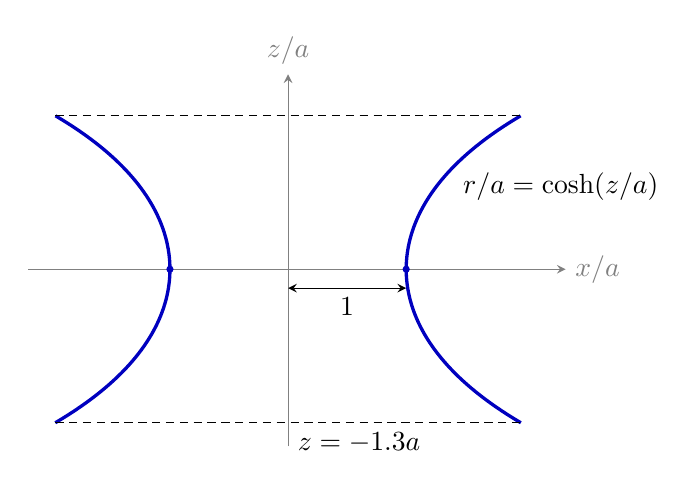
\begin{tikzpicture}[x=1.5cm,y=1.5cm,>=stealth]
	\draw[->,gray] (-2.2,0)--(2.35,0) node[right] {\(x/a\)};
	\draw[->,gray] (0,-1.5)--(0,1.65) node[above] {\(z/a\)};
	\draw[very thick,blue!75!black,domain=-1.3:1.3,samples=81]
		plot ({cosh(\x)},\x);
	\draw[very thick,blue!75!black,domain=-1.3:1.3,samples=81]
		plot ({-cosh(\x)},\x);
	\draw[densely dashed] (-1.97091,1.3)--(1.97091,1.3);
	\draw[densely dashed] (-1.97091,-1.3)--(1.97091,-1.3);
	\draw[<->] (0,-.16)--(1,-.16) node[midway,below] {\(1\)};
	\fill[blue!75!black] (1,0) circle (1.3pt);
	\fill[blue!75!black] (-1,0) circle (1.3pt);
	\node[right] at (1.4,.7) {\(r/a=\cosh(z/a)\)};
	\node[below right] at (0,-1.3) {\(z=-1.3a\)};
\end{tikzpicture}

	\caption{悬链面与过旋转轴平面的交线。将右支绕竖轴旋转得到整张曲面；颈圈半径为 \(a\)。在颈圈之外可分别写成上、下两张水平图，颈圈处则使用 \((v,\theta)\) 参数。}
	\label{g3:fig:catenoid-profile}
\end{figure}

图\ref{g3:fig:catenoid-profile}给出了悬链面的旋转轮廓。上述参数的全局性质也能直接看出。悬链面的第三坐标确定 \(v\)，前两坐标再确定 \(\theta\) 模 \(2\pi\)，故它是嵌入；紧集的原像使 \(v\) 有界，因而原像紧。螺旋面的第三坐标确定实数 \(\theta\)，前两坐标再确定 \(s\)，所以它也是适当嵌入。这里“适当”指紧集的原像为紧集，后面用它保证环境球内的参数面积有限。
\ProseParagraphBreak
两者的共形度量均不小于 \(a^2(\mathrm dv^2+\mathrm d\theta^2)\)。若一列点关于诱导距离为 Cauchy 列，则它关于平坦圆柱或平面距离也为 Cauchy 列，因而收敛；在极限附近两个光滑度量局部等价，遂也按诱导距离收敛。这证明两曲面完备。螺旋面的 \(\theta\) 不能模 \(2\pi\) 取商，否则第三坐标改变 \(2\pi a\)；这正是局部等距不能自动变成整体同一参数空间的原因。

\subsection{共形参数与局部 Weierstrass 表示}
\label{g3:subsec:1902:04}
对一般光滑极小浸入曲面，先在诱导度量上使用\cref{g3:lem:surface-isothermal-coordinate}，即可选择局部共形坐标。\Cref{g3:prop:conformal-harmonic-minimal}随后把极小性识别为三个坐标函数的调和性。Weierstrass 表示将这个描述进一步改写成全纯数据。\footnote{Karl Theodor Wilhelm Weierstrass（1815--1897），德国数学家，研究复函数、幂级数、椭圆函数与变分法。}

\begin{theorem}[局部 Weierstrass 表示]\label{g3:thm:local-weierstrass-representation}
	设 \(D\subset\mathbb C\) 为开圆盘，\(\phi_1,\phi_2,\phi_3\) 为全纯函数，满足
	\begin{equation}\label{g3:eq:weierstrass-null-condition}
		\phi_1^2+\phi_2^2+\phi_3^2=0,\qquad
		|\phi_1|^2+|\phi_2|^2+|\phi_3|^2>0.
	\end{equation}
	则对固定 \(z_0\in D\) 和 \(p\in\mathbb R^3\)，公式
	\begin{equation}\label{g3:eq:weierstrass-null-integral}
		F(z)=p+\operatorname{Re}\int_{z_0}^z(\phi_1,\phi_2,\phi_3)\,\mathrm d\zeta
	\end{equation}
	定义共形极小浸入，积分在 \(D\) 中与路径无关，诱导度量为
	\(\frac12\sum_\alpha|\phi_\alpha|^2|\mathrm dz|^2\)。反过来，每个到 \(\mathbb R^3\) 的光滑极小曲面浸入，在局部等温参数中均由此得到。
	在适当刚性旋转后缩小圆盘，还可写成
	\begin{equation}\label{g3:eq:weierstrass-fg-data}
		(\phi_1,\phi_2,\phi_3)
		=f(1-g^2,\ i(1+g^2),\ 2g),
	\end{equation}
	其中 \(f,g\) 全纯且 \(f\ne0\)，此时诱导度量为
	\begin{equation}\label{g3:eq:weierstrass-metric}
		g_F=|f|^2(1+|g|^2)^2|\mathrm dz|^2.
	\end{equation}
\end{theorem}
\begin{proof}
	全纯一形式 \(\phi_\alpha\,\mathrm dz\) 是闭的，因为其外微分等于 \(\partial_{\bar z}\phi_\alpha\,\mathrm d\bar z\wedge\mathrm dz=0\)。圆盘为星形，沿从 \(z_0\) 出发的线段积分即得原函数；对线段积分求导，或使用\cref{g3:lem:surface-isothermal-coordinate}证明中的径向原函数计算，得到其微分正是该一形式。因此沿任何路径的积分都等于原函数的端点差。
	写 \(\phi=(\phi_1,\phi_2,\phi_3)=a+ib\)，其中 \(a,b\) 为实向量，则
	\[
		F_x=a,\qquad F_y=-b.
	\]
	复双线性恒等式 \(\phi\cdot\phi=0\) 分别给出
	\(|a|^2=|b|^2\)、\(a\cdot b=0\)。非退化条件使两者都非零，故 \(F\) 共形浸入，且共形因子为 \(|a|^2=\frac12|\phi|^2\)。全纯原函数的实部调和，直接由 Cauchy--Riemann 方程也得到 \(F_{xx}+F_{yy}=0\)。所以\cref{g3:prop:conformal-harmonic-minimal}给出极小性。
	反过来，给极小浸入的诱导度量选等温坐标。写
	\(\phi=F_x-iF_y\)，则
	\[
		\partial_{\bar z}\phi=\tfrac12(F_{xx}+F_{yy})=0.
	\]
	共形性给出 \(\phi\cdot\phi=0\)，浸入性给出 \(\phi\ne0\)。又 \(\mathrm dF=\operatorname{Re}(\phi\,\mathrm dz)\)，故恢复积分表达式。
	最后，在中心适当选择环境正交坐标，使 \(\phi_1-i\phi_2\ne0\)；例如可将两个共形切向量分别送到正 \(x_1\) 轴和负 \(x_2\) 轴。缩小圆盘使该函数处处非零，令
	\[
		f=\frac{\phi_1-i\phi_2}{2},\qquad
		g=\frac{\phi_3}{2f}.
	\]
	零二次式给出 \((\phi_1-i\phi_2)(\phi_1+i\phi_2)=-\phi_3^2\)，于是
	\(\phi_1+i\phi_2=-2fg^2\)。解这两条线性等式便得式\eqref{g3:eq:weierstrass-fg-data}。展开平方模有
	\[
		|1-g^2|^2+|1+g^2|^2+4|g|^2=2(1+|g|^2)^2,
	\]
	代入度量公式即得式\eqref{g3:eq:weierstrass-metric}。
\end{proof}

这个局部版本不需要假定整张曲面已有单个复坐标。若在一个更大的黎曼曲面上给定三个全纯一形式 \(\Phi_\alpha\)，零二次式与非退化条件按坐标变换保持；它们定义全局单值映射的充要条件是
\begin{equation}\label{g3:eq:weierstrass-real-period}
	\operatorname{Re}\int_\gamma(\Phi_1,\Phi_2,\Phi_3)=0
	\quad\text{对每条分段光滑闭路 }\gamma.
\end{equation}
必要性来自对 \(\mathrm dF\) 积分；充分性来自两条端点相同的路径拼成闭路，实部积分因而相同。非零的纯虚周期可以允许，要求复周期本身全为零则过强。
\ProseParagraphBreak
公式中的 \(g\) 也可以是亚纯函数，但须先保证三个一形式实际全纯。在式\eqref{g3:eq:weierstrass-fg-data}中，若 \(g\) 在一点有 \(k\) 阶极点，\(f\) 必须至少有 \(2k\) 阶零点才能消去全部极点；恰为 \(2k\) 阶时至少一个分量在该点非零，仍为浸入。若三个全纯分量同时消失，而并非全部恒零，取最小消失阶 \(\ell\ge1\)，可写 \(\phi=(z-z_*)^\ell\psi\)、\(\psi(z_*)\ne0\)。幂级数的零点性质见第四卷第1.1.3小节。于是
\[
	g_F=\tfrac12|z-z_*|^{2\ell}|\psi(z)|^2|\mathrm dz|^2.
\]
映射仍光滑、调和且弱共形，\(z_*\) 是微分消失 \(\ell\) 阶的孤立分支点；在那里没有正定诱导度量。这项结论来自当前 Euclid 目标的全纯表示，不能无条件移到任意目标的弱共形映射。
% 跨卷依赖：g4:prop:0101:zero-order；g4:thm:0101:identity。
\ProseParagraphBreak
最后，\(f=1\)、\(g=z\) 给出
\[
	F(z)=\operatorname{Re}(z-z^3/3,\ i(z+z^3/3),\ z^2),
\]
度量为 \((1+|z|^2)^2|\mathrm dz|^2\)，与\cref{g3:ex:enneper-branched-parametrization}的直接计算一致。全纯数据保证局部浸入和极小性；它本身不保证整体单射、适当性或完备性，这些性质仍须逐个模型核对。
% 纲要条目排为编号小节标题，并进入目录与书签；说明段仍保留于纲要注释中。

% !TeX root = ../../Book3.tex
% 纲要标题：### 19.3 单调性和稳定不等式
% 纲要位置：几何学计划纲要.md，第 2879 行。
% 正文状态：初稿；尚未正式审核。

% 纲要内容开始
% 
% * 径向变分及面积比
% * 环境曲率修正
% * 稳定性与测试函数
% * 面积密度与放大极限
% 
% 纲要内容结束

\section{单调性和稳定不等式}
\label{g3:sec:1903}

在半径为 \(r\) 的 Euclid 球中，过球心的 \(m\) 维平面面积为 \(\omega_m r^m\)，其中 \(\omega_m\) 是 \(\mathbb R^m\) 单位球体积。因此面积除以 \(r^m\) 后，平面给出一个常数。极小子流形的径向驻值公式表明，这个比值向外只能增加；增加量恰好检测径向方向偏离切空间的程度。稳定性则来自另一种信息：对每个紧支法向速度，面积的二阶变化非负。两种工具分别控制尺度和测试函数，不能相互替代。

\subsection{径向变分及面积比}
\label{g3:subsec:1903:01}
面积始终在参数流形上计算。若浸入有重叠，相同像点的不同原像分别贡献面积。以下“适当浸入”指紧集原像紧；在有界环境球中使用这一条件，是为了保证面积和紧支积分均有明确意义。

\begin{lemma}\label{g3:lem:smooth-radial-layer-integration}
	设 \((M^m,g)\) 为光滑无边界黎曼流形，\(m\ge1\)，\(r:M\to[0,R)\) 连续，在 \(r>0\) 处光滑。假设每个 \(\{r\le t\}\)、\(t<R\)，均紧，\(r^{-1}(0)\) 为有限集，且 \(\{r>0,\nabla r=0\}\) 的 \(m\) 维体积为零。记
	\[
		\Gamma_t=\{r=t,\ |\nabla r|>0\},\qquad
		A(t)=\operatorname{Vol}_g\{r<t\}.
	\]
	则对非负可测函数 \(f\) 和 \(0<a<b<R\)，有
	\begin{equation}\label{g3:eq:smooth-radial-layer-formula}
		\int_{a<r<b}f\,\mu_g
		=\int_a^b\left(\int_{\Gamma_t}\frac{f}{|\nabla r|}\,\mu_{\Gamma_t}\right)\mathrm dt.
	\end{equation}
	其中 \(\Gamma_t\) 是可能不紧的光滑超曲面；\(m=1\) 时内层密度是计数密度。特别地，\(A\) 在每个紧半径区间绝对连续，且几乎处处有
	\begin{equation}\label{g3:eq:radial-area-derivative}
		A'(t)=\int_{\Gamma_t}|\nabla r|^{-1}\,\mu_{\Gamma_t}.
	\end{equation}
\end{lemma}
\begin{proof}
	只需在 \(\nabla r\ne0\) 的开集建立公式，因为余集体积为零。在其中取局部坐标 \((t,y^2,\ldots,y^m)\)，第一坐标为 \(t=r\)。把度量矩阵写成分块形式
	\[
		G=\begin{pmatrix}g_{tt}&b^{\mathsf T}\\b&C\end{pmatrix}.
	\]
	等值面的度量矩阵为 \(C\)，而逆矩阵的 \(tt\) 元为
	\(|\nabla r|^2=(g_{tt}-b^{\mathsf T}C^{-1}b)^{-1}\)。行列式消元给出
	\[
		\sqrt{\det G}=\frac{\sqrt{\det C}}{|\nabla r|}.
	\]
	\(m=1\) 时把空矩阵行列式取为 \(1\)，同一公式仍成立。局部积分换元与 Fubini 定理于是给出所需等式。取这一开集上的可数局部有限坐标覆盖及非负单位分解，对非负函数逐项求和，用单调收敛即可得到全局公式。
	以 \(f=1\) 代入，右侧是一个局部可积函数对半径的积分，故 \(A(b)-A(a)\) 等于该积分。这给出绝对连续性与几乎处处的导数公式。任一正半径等值集在正则点附近是超曲面，在临界点部分体积为零，故整个等值集体积为零；因此开球与闭球的面积相同。
\end{proof}

这里仅证明了当前光滑距离函数所需的层积分公式。关键假设是临界集体积为零，下面用极小方程直接验证，而不预先使用第五编的一般余面积公式。

\begin{theorem}[Euclid 极小子流形的面积单调性]\label{g3:thm:euclidean-minimal-monotonicity}
	设 \(m,q\ge1\)，\(F:M^m\to B_R(p)\subset\mathbb R^{m+q}\) 是光滑适当极小浸入，\(M\) 无边界，取诱导度量。令
	\[
		r=|F-p|,\qquad A(t)=\int_{\{r<t\}}\mu_g,\qquad 0<t<R.
	\]
	则对任意 \(0<s<t<R\)，
	\begin{equation}\label{g3:eq:minimal-area-monotonicity}
		\frac{A(t)}{t^m}-\frac{A(s)}{s^m}
		=\int_{s<r<t}\frac{|(F-p)^\perp|^2}{r^{m+2}}\,\mu_g\ge0.
	\end{equation}
	上标 \(\perp\) 表示在每个原像点投影到该支的法空间。等号当且仅当环带 \(s<r<t\) 上的径向向量 \(F-p\) 处处切向。带边界浸入若其边界像避开 \(B_R(p)\)，也有同一结论。
\end{theorem}
\begin{proof}
	记 \(X=F-p\)。\Cref{g3:prop:immersion-position-laplacian}给出
	\[
		\operatorname{div}_M X^\top=m,\qquad
		\nabla_M(r^2/2)=X^\top,\qquad
		|\nabla_Mr|^2=1-\frac{|X^\perp|^2}{r^2}\le1.
	\]
	第一式也可直接由 \(\sum_i\langle\overline\nabla_{e_i}X,e_i\rangle=m\) 及平均曲率为零得到。
	适当性使 \(F^{-1}(p)\) 紧，浸入的局部单射性使它离散，故为有限集。考察 \(h=r^2/2\) 的临界点。在该点 \(\operatorname{tr}\operatorname{Hess}h=m\)，所以至少有一个二阶坐标偏导不为零。于是某个一阶偏导 \(\partial_i h\) 的零集在该点附近是光滑超曲面，临界集包含于其中。用可数覆盖可知整个临界集体积为零。对 \(r>0\)，\(\nabla r=0\) 与 \(\nabla h=0\) 等价，故上一引理适用。
	为了不要求所选半径都是正则值，使用径向截断。设 \(\eta\ge0\) 光滑、在零附近为常数、支于 \([0,R)\)。\(\eta(r)X^\top\) 是紧支光滑切向场，在 \(r=0\) 处也光滑。散度定理给出
	\begin{equation}\label{g3:eq:minimal-radial-cutoff}
		0=\int_M\left(m\eta(r)+r\eta'(r)|\nabla r|^2\right)\mu_g.
	\end{equation}
	令 \(B(t)=\int_{\Gamma_t}|\nabla r|\,\mu_{\Gamma_t}\)。层积分公式使 \(tB(t)\) 在远离零的紧区间可积。取 \(\eta\) 在 \([0,t]\) 为 \(1\)，在长度趋零的外侧过渡区降为 \(0\)，并使用一维可积函数的 Lebesgue 微分定理。对几乎每个 \(t\)，式\eqref{g3:eq:minimal-radial-cutoff}成为
	\begin{equation}\label{g3:eq:minimal-radial-flux}
		mA(t)=t\int_{\Gamma_t}|\nabla r|\,\mu_{\Gamma_t}.
	\end{equation}
	将它与式\eqref{g3:eq:radial-area-derivative}相减，得到几乎处处的恒等式
	\[
		\frac{\mathrm d}{\mathrm dt}\left(t^{-m}A(t)\right)
		=t^{-m}\int_{\Gamma_t}
		\frac{1-|\nabla r|^2}{|\nabla r|}\,\mu_{\Gamma_t}.
	\]
	面积函数绝对连续，故在 \([s,t]\) 上积分合法；再次使用层积分公式，将右侧变成
	\(\int_{s<r<t}(1-|\nabla r|^2)r^{-m}\mu_g\)，即为式\eqref{g3:eq:minimal-area-monotonicity}。
	被积函数连续且非负。若积分为零，它在开环带内处处为零，所以径向向量切向；反方向直接代入即可。若有边界但其像避开球，所用紧支场的支集仍在内部，整个证明不变。
\end{proof}

若径向向量切向，在环带中可令 \(Y\) 为满足 \(\mathrm dF(Y)=F-p\) 的切向场。其局部流满足
\[
	\frac{\mathrm d}{\mathrm d\tau}(F\circ\Phi_\tau-p)
	=F\circ\Phi_\tau-p,
	\qquad F\circ\Phi_\tau-p=e^\tau(F-p).
\]
因而等号表示各支在允许的半径范围内沿射线延伸。较小闭环带的原像紧，保证该流可以延续到给定的内外半径；这就是面积比常数与局部锥形结构之间的准确联系。

\subsection{环境曲率修正}
\label{g3:subsec:1903:02}
环境弯曲时，\(\operatorname{Hess}(r^2/2)\) 不再等于度量。截面曲率上界给出它的下界，足以控制面积比可能出现的下降。以下保留一个明确且便于核对的修正因子。

\begin{theorem}\label{g3:thm:curvature-corrected-area-monotonicity}
	设 \((\overline M^{m+q},\overline g)\) 为完备光滑无边界黎曼流形，\(m,q\ge1\)。固定 \(p\in\overline M\)，取 \(0<R<\operatorname{inj}_{\overline g}(p)\)。假设从 \(p\) 出发、长度小于 \(R\) 的径向测地线沿途每个含径向的二维平面均满足截面曲率 \(K\le\kappa\)，其中 \(\kappa\ge0\)，并且 \(\kappa R^2\le1/2\)。若 \(F:M^m\to B_R^{\overline g}(p)\) 是光滑适当极小浸入、\(M\) 无边界，则
	\begin{equation}\label{g3:eq:curved-minimal-area-ratio}
		r\longmapsto
		e^{m\kappa r^2/2}\frac{\operatorname{Vol}_g(F^{-1}(B_r^{\overline g}(p)))}{r^m}
	\end{equation}
	在 \(0<r<R\) 上单调不减。边界像避开 \(B_R(p)\) 时同样成立。
\end{theorem}
\begin{proof}
	先在环境中记 \(r=d_{\overline g}(p,\cdot)\)。单射半径条件使 \(r\) 在球内除中心外光滑，\(r^2\) 则在中心也光滑。由\cref{g3:thm:hessian-comparison}，
	\[
		\overline{\operatorname{Hess}}r
		\ge\operatorname{ct}_\kappa(r)
		(\overline g-\mathrm dr\otimes\mathrm dr).
	\]
	这里 \(\operatorname{ct}_0(r)=1/r\)，\(\kappa>0\) 时为
	\(\sqrt\kappa\cot(\sqrt\kappa r)\)。令 \(a(r)=r\operatorname{ct}_\kappa(r)\)。在 \(0\le x\le1\) 上有
	\[
		0\le1-x\cot x
		=\frac{\sin x-x\cos x}{\sin x}
		\le x^2.
	\]
	事实上分子为 \(\int_0^x t\sin t\,\mathrm dt\)，介于 \(0\) 与 \(x^3/3\) 之间，而 \(\sin x\ge x-x^3/6\ge5x/6\)；这甚至给出上界 \(2x^2/5\)。因此 \(1-\kappa r^2\le a(r)\le1\)。乘积法则给出
	\[
		\overline{\operatorname{Hess}}(r^2/2)
		\ge a(r)\overline g+(1-a(r))\mathrm dr\otimes\mathrm dr
		\ge(1-\kappa r^2)\overline g.
	\]
	现把 \(r\) 拉回 \(M\)。沿浸入的 Hessian 链式法则为
	\[
		\operatorname{Hess}_M(\psi\circ F)(X,Y)
		=\overline{\operatorname{Hess}}\psi(\mathrm dF X,\mathrm dF Y)
		+\langle\overline\nabla\psi,B(X,Y)\rangle.
	\]
	它由 Gauss 分解直接得到；取迹时后一项为 \(m\langle\overline\nabla\psi,H\rangle=0\)。于是对 \(h=r^2/2\)，
	\begin{equation}\label{g3:eq:curved-radial-divergence}
		\operatorname{div}_M\nabla h\ge m(1-\kappa r^2)\ge m/2,
		\qquad |\nabla_Mr|\le1.
	\end{equation}
	中心原像有限。临界点处 Hessian 的迹严格为正，所以与前一定理相同的一阶偏导零集论证表明临界集体积为零。\Cref{g3:lem:smooth-radial-layer-integration}因而适用。
	对非负径向截断 \(\eta\)，积分 \(\operatorname{div}(\eta(r)\nabla h)\)，用式\eqref{g3:eq:curved-radial-divergence}，得到
	\[
		0\ge m\int\eta(r)(1-\kappa r^2)\mu_g
		+\int\eta'(r)r|\nabla r|^2\mu_g.
	\]
	令截断逼近半径 \(t\) 的球示性函数，得到几乎处处
	\[
		t\int_{\Gamma_t}|\nabla r|\,\mu_{\Gamma_t}
		\ge m\int_{r<t}(1-\kappa r^2)\mu_g
		\ge m(1-\kappa t^2)A(t).
	\]
	因 \(|\nabla r|\le1\)，层积分导数满足
	\(tA'(t)\ge t\int_{\Gamma_t}|\nabla r|\)。故
	\[
		\frac{\mathrm d}{\mathrm dt}\left(e^{m\kappa t^2/2}t^{-m}A(t)\right)
		=e^{m\kappa t^2/2}t^{-m}
		\left(A'(t)-\frac m t A(t)+m\kappa t A(t)\right)\ge0
	\]
	几乎处处成立。局部绝对连续性把它提升为全部半径间的单调性。全部截断支于球内，边界版本也随之成立。
\end{proof}

这个版本只用径向截面曲率的上界；非正截面曲率时可取 \(\kappa=0\)，在割点以前无需指数修正。正曲率下，无修正的面积比确实可能下降。例如单位圆球中的全测地 \(S^2\subset S^3\)，以曲面上一点为中心，充分小的环境球截得的曲面面积是 \(2\pi(1-\cos r)\)。其面积比为
\[
	\frac{2\pi(1-\cos r)}{r^2}
	=\pi\left(1-\frac{r^2}{12}+O(r^4)\right).
\]
它在小半径处向外下降，而上述修正因子补偿了这一曲率误差。若球已越过割迹，光滑距离及 Hessian 比较的用法也须改变，不能只保留同一个积分式。

\subsection{稳定性与测试函数}
\label{g3:subsec:1903:03}
面积驻值使第一变分为零，稳定性进一步要求所有允许的二阶变化非负。在双侧超曲面上，可以固定全局单位法向 \(\nu\)，把法向速度写成 \(f\nu\)。这时稳定性成为一个直接可代入测试函数的积分不等式。

\begin{proposition}\label{g3:prop:stable-minimal-test}
	设 \(F:M^m\to(\overline M^{m+1},\overline g)\)、\(m\ge1\)，为光滑双侧极小超曲面浸入，\(M\) 可有光滑边界。固定光滑单位法向 \(\nu\)，令
	\(V_0=|A|^2+\overline{\operatorname{Ric}}(\nu,\nu)\)。则 \(F\) 对全部内部紧支法向变分稳定，当且仅当
	\begin{equation}\label{g3:eq:minimal-stability-test}
		\int_M V_0 f^2\mu_g\le\int_M|\nabla f|^2\mu_g
		\quad\text{对所有 }f\in C_c^\infty(\operatorname{int}M).
	\end{equation}
	若稳定且在所测区域上 \(\overline{\operatorname{Ric}}(\nu,\nu)\ge-K\)，\(K\ge0\)，则每个相应紧支光滑截断 \(\eta\) 满足
	\[
		\int |A|^2\eta^2\mu_g
		\le\int|\nabla\eta|^2\mu_g+K\int\eta^2\mu_g.
	\]
\end{proposition}
\begin{proof}
	每个内部紧支法向场都唯一写成 \(f\nu\)。因为一维法丛的单位截面满足 \(\nabla^\perp\nu=0\)，式\eqref{g3:eq:minimal-normal-index-form}化为
	\[
		Q(f\nu,f\nu)=\int_M\bigl(|\nabla f|^2-V_0f^2\bigr)\mu_g.
	\]
	其中环境曲率项的求和是 \(\overline{\operatorname{Ric}}(\nu,\nu)\)，第二基本形式项的求和是 \(|A|^2\)。每个这样的场由法向指数变分实现，所以稳定性的量词恰为所述全部测试函数。最后把 Ricci 下界移项即可。
\end{proof}

例如取 \(0\le\eta\le1\)，使其在内域 \(U\) 上为 \(1\)、在宽度 \(d\) 的过渡层 \(E\) 中降为 \(0\)，且 \(|\nabla\eta|\le C/d\)，就得到
\[
	\int_U|A|^2\mu_g
	\le\frac{C^2}{d^2}\operatorname{Vol}(E)
	+K\operatorname{Vol}(\operatorname{supp}\eta).
\]
梯度项只需过渡层的体积，曲率下界中的 \(K\) 项则涉及整个支集。这样的结论是积分估计；要得到逐点曲率界，还需第二基本形式本身满足的微分不等式与迭代论证。

\begin{proposition}\label{g3:prop:positive-jacobi-stability}
	设 \((M,g)\) 为光滑黎曼流形，允许边界，\(V_0\) 为光滑实函数。若内部存在光滑正函数 \(w>0\) 满足
	\(\Delta_gw-V_0w=0\)，其中 \(\Delta_g=-\operatorname{div}\nabla\)，则对每个 \(f\in C_c^\infty(\operatorname{int}M)\)，
	\begin{equation}\label{g3:eq:positive-jacobi-square-identity}
		\int_M(|\nabla f|^2-V_0f^2)\mu_g
		=\int_M w^2\left|\nabla\left(\frac f w\right)\right|^2\mu_g\ge0.
	\end{equation}
	特别地，光滑 Euclid 极小超曲面上若某个固定方向 \(a\) 满足 \(\langle\nu,a\rangle>0\)，则该超曲面稳定；每个光滑标量极小图都满足此条件。
\end{proposition}
\begin{proof}
	写 \(f=w\psi\)。展开平方，并把混合项与 \(\psi^2|\nabla w|^2\) 合并，得到
	\[
		|\nabla f|^2=w^2|\nabla\psi|^2
		+\langle\nabla w,\nabla(w\psi^2)\rangle.
	\]
	在紧支集上积分分部，第二项成为 \(\int(\Delta w)w\psi^2\mu_g=\int V_0f^2\mu_g\)，即得平方恒等式。正性保证除以 \(w\) 在每个紧支集上光滑，并不要求它在整个非紧流形上有统一正下界。
	为处理法向分量，取 Euclid 超曲面的局部正交标架，在一点令源联络系数为零。写 \(h_{ij}=\langle B(e_i,e_j),\nu\rangle\)，则 \(\overline\nabla_{e_i}\nu=-\sum_jh_{ij}e_j\)。再求一次导数并取迹，得到环境向量恒等式
	\[
		\sum_i\left(\overline\nabla_{e_i}\overline\nabla_{e_i}\nu
		-\overline\nabla_{\nabla_{e_i}e_i}\nu\right)
		=-\sum_j\left(\sum_i\nabla_i h_{ij}\right)e_j-|A|^2\nu.
	\]
	\Cref{g3:thm:codazzi-equation}在平坦环境给出
	\(\sum_i\nabla_i h_{ij}=\nabla_j\sum_i h_{ii}=0\)，最后一步用极小性。因此逐个环境坐标有 \(\Delta\nu=|A|^2\nu\)。与常向量 \(a\) 配对，\(w=\langle\nu,a\rangle\) 就满足 \((\Delta-|A|^2)w=0\)。平方恒等式与上一命题给出稳定性。对向上极小图，\(a=e_{m+1}\)、\(w=(1+|\mathrm Du|^2)^{-1/2}>0\)，故条件成立。
\end{proof}

一个整体极小曲面可以由稳定图小片覆盖而本身不稳定。悬链面就是这种情形：\cref{g3:ex:catenoid-unstable-test}将用一个跨越颈圈的紧支函数给出负二阶变化。局部正的法向分量未必能够拼成全局正 Jacobi 函数。高余维时法向场还具有多个耦合分量，稳定性应直接使用式\eqref{g3:eq:minimal-normal-index-form}，不能无条件压缩成上述单个标量势。

\subsection{面积密度与放大极限}
\label{g3:subsec:1903:04}
将面积比再除以单位球体积，定义
\[
	\Theta_p(r)=\frac{A(r)}{\omega_mr^m}.
\]
Euclid 情形中它单调不减且非负，故 \(r\downarrow0\) 时存在有限极限：对任意固定 \(r_0\)，\(0\le\Theta_p(r)\le\Theta_p(r_0)<\infty\)。记这一极限为 \(\Theta_p(0)\)，称它为中心处的面积密度。曲率修正版本也给出同一极限的存在，因为指数因子趋于 \(1\)。

\begin{proposition}\label{g3:prop:smooth-immersion-density}
	设 \(F:M^m\to\mathbb R^{m+q}\)、\(m,q\ge1\)，为光滑适当浸入，\(M\) 无边界，取诱导度量，不要求极小。则对任意 \(p\in\mathbb R^{m+q}\)，中心原像数 \(k=\#F^{-1}(p)\) 有限，且
	\begin{equation}\label{g3:eq:smooth-immersion-density}
		\lim_{r\downarrow0}\frac{\operatorname{Vol}_g\{|F-p|<r\}}{\omega_mr^m}=k.
	\end{equation}
	在每个原像点附近，将像平移并放大 \(r^{-1}\)，所得单支以光滑图的方式在紧集上趋于其切平面。各支分别计数，即使某些切平面相同，也不合并重数。
\end{proposition}
\begin{proof}
	浸入局部为嵌入，故 \(F^{-1}(p)\) 离散；适当性使其紧，所以有限。设原像为 \(x_1,\ldots,x_k\)，取互不相交的源邻域。存在足够小的环境球，其全部原像都落在这些邻域中：否则有球心趋于 \(p\) 的像点而原像在邻域之外，适当性使这些原像在某个固定闭球的原像中取收敛子列，极限既映到 \(p\) 又不在所选邻域，矛盾。\(k=0\) 时同一论证表明充分小球原像为空。
	把每一支旋转为其切平面上的图，可写
	\[
		F(x)=p+(x,v(x)),\qquad v(0)=0,\quad\mathrm Dv(0)=0.
	\]
	在足够小邻域，\(|v(x)|\le C|x|^2\)、\(|\mathrm Dv(x)|\le C|x|\)。若 \(|x|<r(1-C_1r^2)\)，取固定足够大的 \(C_1\) 后便有 \(|(x,v(x))|<r\)；反方向 \(|(x,v(x))|<r\) 必有 \(|x|<r\)。图面积密度
	\(\sqrt{\det(I+(\mathrm Dv)^{\mathsf T}\mathrm Dv)}=1+O(|x|^2)\)。因此该支的球内面积为 \(\omega_mr^m(1+O(r^2))\)。有限支相加得到式\eqref{g3:eq:smooth-immersion-density}。
	放大后的图函数为 \(v_r(y)=r^{-1}v(ry)\)。在固定紧集上，零阶和一阶范数均为 \(O(r)\)；对 \(j\ge2\)，
	\(\mathrm D^jv_r(y)=r^{j-1}(\mathrm D^jv)(ry)\to0\)。这就证明各阶导数都趋于切平面图函数零。
\end{proof}

因此在光滑适当嵌入点，密度为 \(1\)，放大极限就是唯一切平面；在浸入自交点，多个平面及其重数来自多个源点。面积单调性于是还给出极小浸入的下界 \(A(r)\ge k\omega_mr^m\)，只要球不遇边界。
\ProseParagraphBreak
把集合 \(C\subset\mathbb R^{m+q}\) 称为以原点为顶点的锥，是指 \(tC=C\) 对所有 \(t>0\) 成立。若去掉顶点后它是光滑子流形，则径向向量处处切向；反过来，径向场的流把每个局部片沿射线延伸。面积单调性的等号正是在检测这个条件。
\ProseParagraphBreak
对一个已经给定的极小浸入，在尺度 \(r_j\downarrow0\) 放大，面积比满足
\[
	\Theta^{(j)}_0(R)=\Theta_p(r_jR).
\]
所以任意固定 \(0<a<b\)，两端面积比之差趋于零。由式\eqref{g3:eq:minimal-area-monotonicity}，放大后在该环带的径向法向分量平方的加权积分也趋于零。若另外已知这些放大曲面在环带内以固定有限重数局部光滑收敛到光滑极小极限，那么任一极限小片上的该非负积分也是零，径向向量在极限上处处切向。这是“放大极限应当是锥”的一个严格的条件性推论。
\ProseParagraphBreak
面积上界本身尚未提供刚才所假设的光滑收敛。在可能产生奇点的极小曲面列中，须先定义适合的弱对象、证明相应紧性并说明重数如何保留，才谈得上一般切锥的存在或结构。第五编将建立这些工具。当前证明已经给出光滑点的密度与切平面、精确的面积比误差，以及光滑放大极限的径向性；它们说明了弱理论需要保留哪些量。
% 纲要条目排为编号小节标题，并进入目录与书签；说明段仍保留于纲要注释中。

% !TeX root = ../../Book3.tex
% 纲要标题：### 19.4 校准及全局极小性
% 纲要位置：几何学计划纲要.md，第 2886 行。
% 正文状态：初稿；尚未正式审核。

% 纲要内容开始
% 
% * 余范数和校准平面
% * 闭性与同调竞争类
% * 校准原理与体积极小性
% * 复子流形与 Kähler 校准
% * 特殊 Lagrange 模型及非唯一性
% 
% ---
% 
% 纲要内容结束

\section{校准及全局极小性}
\label{g3:sec:1904}

第二变分比较无穷小的邻近曲面。若要与同一个竞争类中的所有曲面比较，需要一个可以在整个类中保持不变的量。闭微分形式的积分正具有这种性质；再使它在每个切平面上的值不超过体积，就得到全局下界。本节完整证明这一校准原理及两个基本代数模型，经典论述见\cite[第II.4节，第59页，定理4.2；第III.1--III.2节，第86--93页]{HarveyLawson1982Calibrated}。

\subsection{余范数和校准平面}
\label{g3:subsec:1904:01}
在 Euclid 空间中，\(\mathrm dx^1\wedge\cdots\wedge\mathrm dx^m\) 测量一个定向 \(m\) 维平行多面体在前 \(m\) 个坐标方向上的带符号投影体积。投影不能增加体积，所以该形式的值始终受原体积控制；在正向水平平面上恰好取等。下面抽出这个性质。

\begin{definition}\label{g3:def:calibration-comass}
	设 \((X^n,g)\) 为光滑无边界黎曼流形，\(1\le m\le n\)，\(\phi\in\Omega^m(X)\)。其在 \(x\) 处的\term[yufanshu]{余范数}[comass]为
	\[
		\|\phi_x\|_*=\sup\{|\phi_x(e_1,\ldots,e_m)|:
		 e_1,\ldots,e_m\text{ 为正交单位向量}\}.
	\]
	若 \(\mathrm d\phi=0\) 且 \(\|\phi_x\|_*\le1\) 对所有 \(x\) 成立，称 \(\phi\) 为一个 \(m\) 次\term[jiaozhun]{校准}[calibration]。有向 \(m\) 平面 \(P\subset\mathrm T_xX\) 若满足 \(\phi_x|_P=\operatorname{vol}_P\)，称为被 \(\phi\) 校准的平面。定向光滑浸入 \(F:M^m\to X\) 若满足 \(F^*\phi=\operatorname{vol}_{F^*g}\)，称为被 \(\phi\) 校准的浸入。
\end{definition}
\symidx{\(\lVert\phi_x\rVert_*\)：微分形式的逐点余范数}

正交标架的集合紧，所以这个上确界能达到。反转定向使形式值变号，故条件 \(\phi(P)=1\) 同时指定了取等平面与它的方向。本书允许某些点的余范数严格小于一；这些点没有被校准的平面，故被校准浸入的像只能经过能取等的点。

\ProseParagraphBreak

余范数与外代数上的 Euclid 范数不同。比如 \(\mathbb R^4\) 上
\(\omega=\mathrm dx^1\wedge\mathrm dy^1+\mathrm dx^2\wedge\mathrm dy^2\) 的外代数范数是 \(\sqrt2\)。但对正交单位 \(u,v\)，有 \(\omega(u,v)=\langle Ju,v\rangle\le1\)，并可取 \(v=Ju\) 达到一，所以余范数为一。余范数只测试代表真实切平面的简单单位多向量。

\subsection{闭性与同调竞争类}
\label{g3:subsec:1904:02}
先说明积分比较中的同调条件。对紧定向光滑 \(m\) 维流形上的映射 \(F\)，用 \([F]\) 表示其带重数的积分区域，即 \([F](\alpha)=\int_MF^*\alpha\)。有限条这样的带系数区域可以相加。若
\begin{equation}\label{g3:eq:calibration-homology-competitors}
	[F_1]-[F_0]=\partial C,
\end{equation}
其中 \(C=\sum_a c_a[G_a:P_a^{m+1}\to X]\) 是有限条紧定向分片光滑区域组成的链，边界按外法向优先取向并将公共面抵消，就称这两个区域在此竞争中同调。允许各 \(P_a\) 有角；光滑奇异单形是其中的基本模型。等式表示对每个 \(m\) 次形式，左右的有向积分相同。

\ProseParagraphBreak

第一卷第14.4.4小节的带角 Stokes 定理给出
\begin{equation}\label{g3:eq:calibration-period-invariance}
	\int_{M_1}F_1^*\phi-\int_{M_0}F_0^*\phi
	=\sum_a c_a\int_{P_a}\mathrm d(G_a^*\phi)=0
\end{equation}
只要 \(\mathrm d\phi=0\)。每条参数区域紧，故即使 \(X\) 非紧也没有无穷远边界项。用光滑奇异链表达时，这就是第二卷第7.3.2小节的积分链映射公式。闭流形上普通同调类的积分不变量正由同一公式给出；这里把可实际用于比较的填充链写明。

\ProseParagraphBreak

固定边界的光滑同伦自动给出所需链：将 \([0,1]\times M\) 映到 \(X\)，其两端是 \(F_1\) 与 \(-F_0\)；侧边 \([0,1]\times\partial M\) 上映射与时间无关，微分秩至多 \(m-1\)，所以任意 \(m\) 次形式在侧边的积分为零。另一方面，仅有相同边界未必能在给定环境中找到式\eqref{g3:eq:calibration-homology-competitors}的填充，比较时要保留这一拓扑条件。

\begin{example}\label{g3:exm:nonclosed-unit-form-circles}
	在穿孔平面上取
	\[
		\alpha=\frac{-y\,\mathrm dx+x\,\mathrm dy}{\sqrt{x^2+y^2}}
		=r\,\mathrm d\theta.
	\]
	它的余范数处处为一，且在每条逆时针圆周上等于弧长形式。然而 \(\mathrm d\alpha=\mathrm dr\wedge\mathrm d\theta\ne0\)，不同半径的圆周虽围成环带，长度仍为 \(2\pi r\) 而不同。逐点取等本身没有提供同调极小性，闭性承担了保持积分的作用。
\end{example}

\subsection{校准原理与体积极小性}
\label{g3:subsec:1904:03}
\begin{theorem}[校准原理]\label{g3:thm:calibrated-volume-minimizing}
	设 \((X^n,g)\) 为光滑无边界黎曼流形，\(1\le m\le n\)，\(\phi\) 为 \(m\) 次校准。设 \(F_i:M_i^m\to X\) 为紧定向光滑流形的光滑浸入，允许光滑边界，且 \([F_1]-[F_0]=\partial C\)，其中 \([F_i](\alpha)=\int_{M_i}F_i^*\alpha\)，\(C\) 为有限条紧定向分片光滑 \((m+1)\) 维参数区域组成的实系数链（可带角），边界取外法向优先定向并抵消公共面，记 \(\mathcal A(F_i)=\operatorname{Vol}(M_i,F_i^*g)\)。若 \(F_0\) 被 \(\phi\) 校准，则
	\[
		\mathcal A(F_0)\le\mathcal A(F_1).
	\]
	等号当且仅当 \(F_1\) 也以给定定向被 \(\phi\) 校准。
\end{theorem}
\begin{proof}
	对 \(F_1\) 在每点选择有向正交单位切标架，余范数条件给出
	\(F_1^*\phi=a\operatorname{vol}_{F_1^*g}\)、\(a\le1\)。于是
	\[
		\mathcal A(F_0)=\int_{M_0}F_0^*\phi
		=\int_{M_1}F_1^*\phi
		\le\int_{M_1}\operatorname{vol}_{F_1^*g}
		=\mathcal A(F_1).
	\]
	第一个等号是 \(F_0\) 的校准性，第二个来自闭性与填充链。若最终取等，连续非负函数 \(1-a\) 的积分为零，故 \(a=1\) 处处；这恰为 \(F_1\) 的校准性。反向直接由同一个等式链得到。
\end{proof}

同一证明适用于光滑带重数的有限竞争链：若以 \(\sum_j|c_j|\operatorname{Vol}(F_j)\) 计算参数体积，就有 \(\int\phi\le\sum_j|c_j|\operatorname{Vol}(F_j)\)。广义弱曲面的质量与紧性将在下一编建立；这里的光滑结论已经能提供不依赖竞争映射接近程度的下界。

\begin{corollary}\label{g3:cor:calibrated-minimal-stable}
	设 \((X,g)\) 为光滑无边界黎曼流形，\(\phi\) 为闭且余范数至多一的 \(m\) 次形式。定向无边界光滑浸入 \(F:M^m\to X\) 若满足 \(F^*\phi=\operatorname{vol}_{F^*g}\)，则它极小，并且对内域紧支变分稳定。紧源带边界时，对固定边界变分也有相同结论；非紧带边界源还要求变分具有紧支集。
\end{corollary}
\begin{proof}
	在包含变分支集的紧区域上，变分扫出的带角圆柱给出填充链。因此每个充分小的正、负参数都满足 \(\mathcal A(F_t)\ge\mathcal A(F_0)\)。一阶导数为零，二阶导数非负；再用\cref{g3:cor:minimal-area-stationarity}得到 \(H=0\)。
\end{proof}

水平平面提供最直接的应用。取 \(\phi=\mathrm dx^1\wedge\cdots\wedge\mathrm dx^m\)，它闭且余范数为一，任何正向水平域都被校准。在 Euclid 环境中，这个形式还恰当：
\(\phi=\mathrm d(x^1\mathrm dx^2\wedge\cdots\wedge\mathrm dx^m)\)，\(m=1\) 时括号中就是函数 \(x^1\)。所以只要两个紧竞争浸入具有相同的有向边界积分区域，它们的 \(\phi\) 积分就相等；平面域在这些竞争者中面积最小。

\subsection{复子流形与 Kähler 校准}
\label{g3:subsec:1904:04}
令 \(J\) 为实内积空间 \(V^{2n}\) 上的正交复结构，\(\omega(u,v)=\langle Ju,v\rangle\)。复 \(k\) 平面的定向规定为
\((e_1,Je_1,\ldots,e_k,Je_k)\)。以下 Wirtinger 不等式\footnote{Wilhelm Wirtinger（1865--1945），奥地利数学家，研究复分析、几何与代数函数。}把复方向转成体积下界。

\termidx[Wirtinger budengshi]{Wirtinger 不等式}
\foreignidx{Wirtinger inequality}
\begin{proposition}[Wirtinger 不等式]\label{g3:prop:wirtinger-calibration}
	设 \((V^{2n},g,J)\) 为 Hermite 实向量空间，\(1\le k\le n\)。令 \(\omega(v,w)=g(Jv,w)\)，则 \(\omega^k/k!\) 的余范数为一；一个有向实 \(2k\) 平面取正等号，当且仅当它由 \(J\) 保持且取复定向。
\end{proposition}
\begin{proof}
	对实平面 \(P\subset V\)，令 \(T=\pi_PJ|_P\)。这是 \(P\) 上的斜自伴算子，范数至多一。说明其正交块形式：\(-T^2\) 自伴非负，若 \(u\) 为单位特征向量、特征值 \(\lambda^2>0\)，则令 \(v=Tu/\lambda\)，得到 \(Tu=\lambda v\)、\(Tv=-\lambda u\)；这个二维空间的正交补仍由 \(T\) 保持，归纳处理即可，核中的方向再两两配对。因此可取正交基，使
	\[
		\omega|_P=\sum_{a=1}^k\lambda_a u^a\wedge v^a,
		\qquad 0\le\lambda_a\le1.
	\]
	故 \(\omega^k/k!\) 在这组基上的值为 \(\prod_a\lambda_a\)，对任意定向的绝对值都至多一。复平面取 \(v_a=Ju_a\) 时全为一，所以余范数确为一。
	绝对值取等迫使所有 \(\lambda_a=1\)。此时每个 \(u\in P\) 都满足 \(|\pi_PJu|=|Ju|\)，所以 \(Ju\in P\)，即 \(P\) 复不变。反过来，复不变平面上总可选 \(u_a,Ju_a\)；它们给出正等号，反定向则给负等号。
\end{proof}

流形上的应用只需要一个光滑正交 \(J\) 及闭的基本二形式 \(\omega\)：外微分乘积公式使 \(\mathrm d(\omega^k)=0\)，上面逐点证明的余范数控制遂说明 \(\omega^k/k!\) 是校准。若 \(J\) 平行，则 \(\omega\) 平行，无挠性给出 \(\mathrm d\omega=0\)；这恢复\cref{g3:def:parallel-kahler-structure}采用的 Kähler 条件，无须借助特殊完整群的分类。

\begin{corollary}\label{g3:cor:complex-submanifold-calibrated}
	设 \((X^{2n},g,J)\) 为光滑 Kähler 流形，\(1\le k\le n\)。记 \(\omega(V,W)=g(JV,W)\) 为 Kähler 形式。若光滑浸入 \(F:M^{2k}\to X\) 的切空间由 \(J\) 保持，则按复定向，它被 \(\omega^k/k!\) 校准，因而极小且局部稳定；对每个带光滑边界的紧定向片 \(M_0\subset M\)，其限制浸入 \(F_0\) 的体积不超过任意同边界定向紧浸入 \(F_1\) 的体积，只要 \([F_1]-[F_0]=\partial C\)，其中 \(C\) 是有限条紧定向分片光滑参数区域组成的填充链。特别地，这适用于 Kähler 流形的光滑复子流形。
\end{corollary}
\begin{proof}
	切空间的复定向在光滑换架下相容，因为复可逆矩阵的实行列式为复行列式模平方，严格为正。Wirtinger 不等式的取等条件逐点给出所需校准等式，再应用校准原理和前一推论。
\end{proof}

例如 \(z\mapsto(z,z^2)\) 把复平面嵌入 \(\mathbb C^2\)。导数复线性且第一分量恒为一，故它是光滑复曲线，参数域上的度量为 \((1+4|z|^2)|\mathrm dz|^2\)。每个紧片都被标准 \(\omega\) 校准。其面积最小性允许竞争面失去复结构，只要求保留相应的边界及同调条件。

\subsection{特殊 Lagrange 模型及非唯一性}
\label{g3:subsec:1904:05}
在 \(\mathbb C^n\) 上取标准度量、\(\omega=\sum_j\mathrm dx^j\wedge\mathrm dy^j\) 及复体积形式
\(\Omega=\mathrm dz^1\wedge\cdots\wedge\mathrm dz^n\)。实 \(n\) 平面 \(P\) 若满足 \(\omega|_P=0\)，称为 Lagrange 平面；等价地 \(JP=P^\perp\)。这一等价由 \(\omega(u,v)=\langle Ju,v\rangle\) 和维数立即得到。流形的切平面满足同一条件时，也称为 Lagrange 子流形。

\begin{proposition}\label{g3:prop:special-lagrangian-calibration}
	给定 \(n\ge1\)、\(\theta\in\mathbb R\)，在 \(\mathbb C^n\) 上取标准 Euclid 度量，\(\Omega=\mathrm dz^1\wedge\cdots\wedge\mathrm dz^n\)、\(\omega=\tfrac{\mathrm i}2\sum_j\mathrm dz^j\wedge\mathrm d\bar z^j\)。有向实 \(n\) 平面上 \(\omega\) 限制为零称为 Lagrange 平面。常系数形式
	\(\phi_\theta=\operatorname{Re}(e^{-\mathrm i\theta}\Omega)\) 是 \(\mathbb C^n\) 上的校准。它校准的平面恰是具有相位 \(\theta\) 的有向 Lagrange 平面，即对正向实正交单位基有 \(\Omega(e_1,\ldots,e_n)=e^{\mathrm i\theta}\)。相应浸入称为\term[teshu lagrange ziliuxing]{特殊 Lagrange 子流形}[special Lagrangian submanifold]。
\end{proposition}
\begin{proof}
	将实正交单位向量 \(e_1,\ldots,e_n\) 视作 \(\mathbb C^n\) 中的列，组成复矩阵 \(Z\)。每列 Hermite 长度为一，Gram--Schmidt 正交化给出 \(|\det_{\mathbb C}Z|\le1\)：行列式的模等于逐次正交投影后各列长度之积，每个长度至多一。取等当且仅当各列复正交，即它们的 Hermite 内积都是 \(\delta_{ij}\)。实部已由实正交性保证，虚部为 \(\omega(e_i,e_j)\) 的正号或负号，故取等恰要求 \(P\) 为 Lagrange。
	又 \(\Omega(e_1,\ldots,e_n)=\det_{\mathbb C}Z\)，从而
	\[
		\phi_\theta(e_1,\ldots,e_n)
		\le |\Omega(e_1,\ldots,e_n)|\le1.
	\]
	正等号同时要求模为一、相位为 \(\theta\)。实轴平面的一次酉旋转可实现任意相位，故余范数为一；常系数使 \(\mathrm d\phi_\theta=0\)。
\end{proof}

对于梯度图 \(F(x)=x+\mathrm i\nabla v(x)\)、\(v\in C^\infty(U)\)、\(U\subset\mathbb R^n\) 开，Hessian 对称性给出 \(F^*\omega=0\)，且
\begin{equation}\label{g3:eq:special-lagrangian-graph}
	F^*\Omega=\det(I+\mathrm iD^2v)\,\mathrm dx^1\wedge\cdots\wedge\mathrm dx^n,
	\qquad \mu_{F^*g}=\sqrt{\det(I+(D^2v)^2)}\,\mathrm dx.
\end{equation}
因此按 \(x\) 的标准定向，特殊相位 \(\theta\) 的方程为
\[
	\operatorname{Im}\bigl(e^{-\mathrm i\theta}\det(I+\mathrm iD^2v)\bigr)=0,
	\qquad \operatorname{Re}\bigl(e^{-\mathrm i\theta}\det(I+\mathrm iD^2v)\bigr)>0.
\]
第二个条件固定取等方向。若 \(\lambda_j\) 是 Hessian 的实特征值，可连续选取相位
\(\Theta(D^2v)=\sum_j\arctan\lambda_j\)，方程也就是 \(\Theta=\theta\pmod{2\pi}\)。在连通的选定分支上它是一个常数方程。对任意实对称增量 \(T\)，行列式求导给出
\[
	\mathrm d\Theta_S(T)=\operatorname{Im}\operatorname{tr}((I+\mathrm iS)^{-1}\mathrm iT)
	=\operatorname{tr}((I+S^2)^{-1}T).
\]
所以线性化的主系数正定；当 \(\|D^2v\|\le L\) 时，其特征值位于 \([(1+L^2)^{-1},1]\)，得到统一椭圆性。

\begin{example}\label{g3:exm:harmonic-gradient-calibration}
	在 \(\mathbb R^2\) 上取调和函数 \(v\)。其 Hessian 特征值为 \(\lambda,-\lambda\)，故 \(\det(I+\mathrm iD^2v)=1+\lambda^2>0\)。因此 \(x+\mathrm i\nabla v(x)\) 是零相位特殊 Lagrange 图，其每个紧片有校准给出的面积下界。取
	\(v(x,y)=x^3/3-xy^2\)，则 \(D^2v=\left(\begin{smallmatrix}2x&-2y\\-2y&-2x\end{smallmatrix}\right)\)，相应因子为 \(1+4(x^2+y^2)\)，得到一个非平面显式模型。
\end{example}

校准也解释极小者可能不唯一。在平坦复环面 \(\mathbb R^{2n}/\mathbb Z^{2n}\) 上，\(\omega,\Omega\) 都下降为全局形式。对每个 \(b\in\mathbb R^n/\mathbb Z^n\)，水平环面
\(L_b=\{[x+\mathrm ib]:x\in\mathbb R^n\}\) 都被 \(\operatorname{Re}\Omega\) 校准，体积为一。连接两个 \(b\) 的路径扫出填充链，故这些环面同调并具有相同的最小体积，而作为子集通常不同。取等条件要求竞争者继续被同一形式校准，并不要求它等于原来的子流形。
% 纲要条目排为编号小节标题，并进入目录与书签；说明段仍保留于纲要注释中。

% !TeX root = ../../Book3.tex
% 纲要标题：### 19.5*　体积约束与常平均曲率
% 纲要位置：几何学计划纲要.md，第 2896 行。

% 纲要内容开始
% 
% > 写作范围与外部输入：规划任务：以闭、双侧、嵌入并围成区域的光滑超曲面为主范围，固定环境定向、单位法向与平均曲率归一化，完整推导体积约束的一阶和二阶变分、常平均曲率条件与约束稳定性。用第16章的球面谱或相应已证不等式完成欧氏球面的保体积稳定模型。一般 CMC 存在、分类及 min-max 构造准确外引；不由无约束稳定性替代保体积稳定性。
% 
% * 围成区域、法向与体积变分
% * 体积约束与常平均曲率方程
% * 保体积变分的二阶公式
% * 球面模型与约束稳定性
% * 常平均曲率超曲面的存在与分类
% 
% ---
% 
% 纲要内容结束
% 正文状态：初稿；尚未正式审核。
% 规划任务：以闭、双侧、嵌入并围成区域的光滑超曲面为主范围，固定环境定向、单位法向与平均曲率归一化，完整推导体积约束的一阶和二阶变分、常平均曲率条件与约束稳定性。用第16章的球面谱或相应已证不等式完成欧氏球面的保体积稳定模型。一般 CMC 存在、分类及 min-max 构造准确外引；不由无约束稳定性替代保体积稳定性。

\OptionalSection{体积约束与常平均曲率}{g3:sec:1905}

把一只球缓慢缩小，面积与体积都会减小；若要求体积保持不变，这个最直接的降面积方向便不再允许。体积约束改变的是竞争变分，也因此把极小方程 \(H=0\) 改成常平均曲率方程。本节始终区分平均曲率向量场 \(H\) 与选定法向下的标量平均曲率 \(h_\nu=\langle H,\nu\rangle\)。

\subsection{围成区域、法向与体积变分}
\label{g3:subsec:1905:01}
设 \((\bar M^{m+1},\bar g)\) 是定向光滑无边界黎曼流形，\(m\ge1\)，\(\Omega\subset\bar M\) 是紧的光滑区域，非空边界 \(\Sigma=\partial\Omega\) 为闭光滑嵌入超曲面。区域指连同边界的余维零子流形，允许不连通。取 \(\nu\) 为外单位法向，记诱导度量为 \(g\)，并定义
\[
	\mathcal A(\Sigma)=\int_\Sigma\mu_g,
	\qquad \mathcal V(\Omega)=\int_\Omega\mu_{\bar g},
	\qquad h_\nu=\frac1m\operatorname{tr}A_\nu.
\]
这里 \(A_\nu X=-\bar\nabla_X\nu\)，所以半径 \(R\) 的 Euclid 球面取外法向时有 \(h_\nu=-1/R\)。对于已选区域，法向的正负不是另外自由选择的。

\ProseParagraphBreak

先把邻近区域写成可直接计算的形式。在充分小的 \(\varepsilon>0\) 下，法向指数映射
\[
	\Phi:\Sigma\times(-\varepsilon,\varepsilon)\longrightarrow\bar M,
	\qquad \Phi(x,s)=\exp_x^{\bar g}(s\nu_x)
\]
给出 \(\Sigma\) 的一个管状邻域。这里的统一性只需紧性：在 \((x,0)\) 处，微分是 \((X,a)\mapsto X+a\nu_x\)，为同构；有限覆盖先给出统一的局部可逆范围。若任意缩小范围后仍有不同点映到同一点，便有 \(s_j,t_j\to0\) 及 \(\Phi(x_j,s_j)=\Phi(y_j,t_j)\)。取收敛子列，极限给出 \(x=y\)，这又与 \((x,0)\) 附近的局部单射性矛盾。缩小 \(\varepsilon\) 后，区域在该邻域中恰为 \(s\le0\)。

\ProseParagraphBreak

这些坐标中 \(\partial_s\) 为单位向量并与各个 \(s\) 层正交。确实，沿法向测地线有 \(\bar\nabla_s\partial_s=0\)；若 \(X\) 是由 \(\Sigma\) 上坐标场延拓的变化场，则 \([\partial_s,X]=0\)，从而
\(\partial_s\langle\partial_s,X\rangle=\frac12X|\partial_s|^2=0\)，初值又为零。因此环境体积密度可写成
\[
	\Phi^*\mu_{\bar g}=J(x,s)\,\mu_g\,\mathrm ds,
	\qquad J(x,0)=1,
	\qquad \partial_sJ(x,0)=-m h_\nu(x).
\]
最后一式是平行层面积密度的变化，直接来自式\eqref{g3:eq:normal-area-density-variation}。

\begin{proposition}\label{g3:prop:enclosed-volume-first-variation}
	设 \((\bar M^{m+1},\bar g)\) 为定向光滑无边界黎曼流形，\(m\ge1\)，\(\Omega\) 为具有非空光滑边界 \(\Sigma\) 的紧区域，\(\nu\) 为外单位法向，\(g\) 为边界的诱导度量。令 \(\Phi(x,s)=\exp_x(s\nu_x)\) 为小管状邻域坐标，\(\Phi^*\mu_{\bar g}=J(x,s)\mu_g\,\mathrm ds\)。对充分小的光滑函数 \(w:\Sigma\to\mathbb R\)，令 \(\Sigma_w=\{\Phi(x,w(x)):x\in\Sigma\}\)，并令 \(\Omega_w\) 在管状邻域中由 \(s\le w(x)\) 定义、在邻域外与 \(\Omega\) 相同。则
	\begin{equation}\label{g3:eq:normal-graph-volume}
		\mathcal V(\Omega_w)-\mathcal V(\Omega)
		=\int_\Sigma\int_0^{w(x)}J(x,s)\,\mathrm ds\,\mu_g.
	\end{equation}
	更一般地，设 \(\Omega_t\) 为光滑区域变分，\(F_t:\Sigma\to\partial\Omega_t\) 为光滑参数化且 \(F_0\) 为包含映射。记 \(g_t=F_t^*\bar g\)、\(f_t=\langle\partial_tF_t,\nu_t\rangle\)，其中 \(\nu_t\) 是区域的外单位法向，则
	\begin{equation}\label{g3:eq:enclosed-volume-first-variation}
		\mathcal V'(t)=\int_\Sigma f_t\,\mu_{g_t}.
	\end{equation}
	若初速度为 \(f\nu\)，再记 \(a=\langle\bar\nabla_t\partial_tF_t|_0,\nu\rangle\)，则
	\begin{equation}\label{g3:eq:enclosed-volume-second-variation}
		\mathcal V''(0)=\int_\Sigma\bigl(a-m h_\nu f^2\bigr)\,\mu_g.
	\end{equation}
\end{proposition}
\begin{proof}
	新旧区域只在管状邻域中不同，沿每条法向线积分便得到式\eqref{g3:eq:normal-graph-volume}；当 \(w<0\) 时，内积分的负号正好记录被去掉的体积。此类图确实由区域变分产生：取在 \(s=0\) 附近等于一、在邻域端部等于零的截断函数 \(\chi(s)\)，以
	\((x,s)\mapsto(x,s+\chi(s)w(x))\)
	作变换。对充分小的 \(w\)，其沿 \(s\) 的导数为正，故是管状邻域的微分同胚，并能在外部延拓为恒等映射。

	对于一般区域变分，先将边界速度光滑延拓为邻域内的向量场，再用截断延拓到环境。其局部流实现同样的瞬时边界速度。流拉回环境密度的导数为 \((\operatorname{div}_{\bar g}W)\mu_{\bar g}\)：在一点取正交坐标，对 Jacobian 行列式求导即得此式。于是\cref{g3:thm:divergence-theorem}给出
	\[
		\mathcal V'(t)=\int_{\Omega_t}\operatorname{div}_{\bar g}W_t\,\mu_{\bar g}
		=\int_{\partial\Omega_t}\langle W_t,\nu_t\rangle\,\mu_{g_t}.
	\]
	结果只取决于边界速度，与延拓无关。对光滑嵌入族，这个延拓可在随时间变化的管状坐标中构造，因而也适用于给定的 \(F_t\)。

	最后对一阶公式求导。初速度为法向时，\(\dot\mu=-m h_\nu f\mu_g\)；由 \(\langle\nu_t,\nu_t\rangle=1\)，有
	\[
		\dot f_0
		=\langle\bar\nabla_t\partial_tF_t|_0,\nu\rangle
		+\langle f\nu,\bar\nabla_t\nu_t|_0\rangle=a.
	\]
	故 \(\mathcal V''(0)=\int(a-m h_\nu f^2)\mu_g\)。
\end{proof}

一阶保体积条件因此是 \(\int_\Sigma f\mu_g=0\)。但这还没有保证某条已选的变分在所有小时间都保持体积；下一小节将补上这个实现步骤。

\subsection{体积约束与常平均曲率方程}
\label{g3:subsec:1905:02}
称光滑区域变分 \(\Omega_t\) 为\term[baotiji bianfen]{保体积变分}[volume-preserving variation]，是指在一个包含零的时间区间上有 \(\mathcal V(\Omega_t)=\mathcal V(\Omega_0)\)。定义中的等式对每个小时间成立。

\begin{lemma}\label{g3:lem:exact-volume-preserving-variation}
	设 \(\Omega\) 为定向光滑无边界黎曼流形 \(\bar M^{m+1}\) 中的紧光滑区域，\(m\ge1\)，边界 \(\Sigma\ne\varnothing\)，外单位法向为 \(\nu\)。光滑函数 \(f:\Sigma\to\mathbb R\) 能实现为一条保体积光滑区域变分的法向初速度 \(f\nu\)，当且仅当
	\[
		\int_\Sigma f\,\mu_g=0.
	\]
\end{lemma}
\begin{proof}
	必要性由体积一阶公式给出。反之，取光滑函数 \(\psi\) 满足 \(\int_\Sigma\psi\mu_g\ne0\)，例如 \(\psi=1\)。使用上面的管状坐标，把两个小实参数 \((t,s)\) 对应的边界写成法向图
	\[
		w(t,s,x)=t f(x)+s\psi(x),
		\qquad G(t,s)=\mathcal V(\Omega_{w(t,s)})-\mathcal V(\Omega).
	\]
	式\eqref{g3:eq:normal-graph-volume}表明 \(G\) 光滑，并且
	\[
		G(0,0)=0,\qquad
		G_s(0,0)=\int_\Sigma\psi\mu_g\ne0,\qquad
		G_t(0,0)=\int_\Sigma f\mu_g=0.
	\]
	第一卷第11.3.2小节的带参数隐函数定理给出光滑函数 \(s=s(t)\)，满足 \(s(0)=0\)、\(G(t,s(t))=0\)。这里待解变量是 \(s\)，可逆的偏导数块就是非零数 \(G_s(0,0)\)。对这个恒等式求导得到 \(s'(0)=0\)。因此
	\(F_t(x)=\Phi(x,t f(x)+s(t)\psi(x))\)
	是所需边界变分，初速度恰为 \(f\nu\)。前一命题的截断构造把它实现为光滑区域变分。
\end{proof}

对指定的全局单位法向，若 \(h_\nu\) 为常数，称超曲面有\term[chang pingjun qulv]{常平均曲率}[constant mean curvature]，常缩写为 CMC。若边界不连通，本节说“\(h_\nu\) 为常数”是指所有分支取同一个值；这是只固定总体积时产生的条件。

\begin{theorem}\label{g3:thm:cmc-volume-critical}
	设 \(\Omega\) 为定向光滑无边界黎曼流形 \(\bar M^{m+1}\) 中的紧光滑区域，\(m\ge1\)，非空边界为 \(\Sigma\)，外单位法向为 \(\nu\)。以下条件等价：
	\begin{enumerate}
		\item \(\mathcal A'(0)=0\) 对所有保体积光滑区域变分成立；
		\item \(h_\nu=h_0\) 在整个 \(\Sigma\) 上为同一常数；
		\item 存在常数 \(h_0\)，使泛函
		\begin{equation}\label{g3:eq:cmc-augmented-functional}
			\mathcal F_{h_0}(\Omega')
			=\mathcal A(\partial\Omega')+m h_0\mathcal V(\Omega')
		\end{equation}
		在 \(\Omega\) 处对全部光滑区域变分驻值。
	\end{enumerate}
\end{theorem}
\begin{proof}
	由面积与体积一阶公式，法向速度 \(f\) 满足
	\[
		\mathcal A'(0)=-m\int_\Sigma h_\nu f\,\mu_g,
		\qquad
		\mathcal F_{h_0}'(0)=-m\int_\Sigma(h_\nu-h_0)f\,\mu_g.
	\]
	切向速度的面积贡献为散度，闭边界上积分为零，也不改变体积。设第一个条件成立，取
	\[
		\bar h=\frac1{\mathcal A(\Sigma)}\int_\Sigma h_\nu\mu_g,
		\qquad f=h_\nu-\bar h.
	\]
	该函数积分为零，由前一引理可实现为精确保体积变分。因此
	\(0=\mathcal A'(0)=-m\int_\Sigma(h_\nu-\bar h)^2\mu_g\)，得到 \(h_\nu=\bar h\)。反之，若 \(h_\nu=h_0\)，保体积条件使 \(\int f=0\)，所以面积一阶导数为零。这证明前两项等价。

	若 \(h_\nu=h_0\)，第二个积分对所有 \(f\) 消失。反过来，任何光滑 \(f\) 都可用法向图实现；取 \(f=h_\nu-h_0\) 即知第三项迫使第二项成立。
\end{proof}

因此乘子是 \(m h_0\)。在外向球面上它等于 \(-m/R\)，乘子泛函为 \(\mathcal A-(m/R)\mathcal V\)。若分别固定各个区域分支的体积，允许的速度在每个区域分支的整个边界上分别积分为零，结论则允许不同区域分支对应不同的平均曲率常数。

\subsection{保体积变分的二阶公式}
\label{g3:subsec:1905:03}
在 CMC 边界处直接对面积求两次导数，会出现加速度项。乘子泛函在所有方向上都驻值，恰好把这些项消去；再限制到精确保体积变分，就得到面积真正的约束二次型。

\begin{theorem}\label{g3:thm:cmc-volume-second-variation}
	设 \(\Omega\) 为定向光滑无边界黎曼流形 \((\bar M^{m+1},\bar g)\) 中的紧光滑区域，\(m\ge1\)，其非空边界 \(\Sigma\) 对外单位法向 \(\nu\) 满足 \(h_\nu=h_0\)。令
	\[
		c_\Sigma=|A_\nu|^2+\overline{\operatorname{Ric}}(\nu,\nu).
	\]
	对法向初速度 \(f\nu\) 的任意光滑区域变分，乘子泛函满足
	\begin{equation}\label{g3:eq:cmc-volume-index-form}
		\mathcal F_{h_0}''(0)=Q_\Sigma(f,f),
		\qquad Q_\Sigma(f,k)=\int_\Sigma
		\bigl(\langle\mathrm df,\mathrm dk\rangle-c_\Sigma f k\bigr)\,\mu_g.
	\end{equation}
	若变分精确保体积，则 \(\mathcal A''(0)=Q_\Sigma(f,f)\)，且 \(\int_\Sigma f\mu_g=0\)。反之，每个光滑零均值 \(f\) 都能由这种变分实现。
\end{theorem}
\begin{proof}
	对变分的每个时刻，设 \(f_t=\langle\partial_tF_t,\nu_t\rangle\)。闭边界上的一阶公式给出
	\[
		\mathcal F_{h_0}'(t)
		=-m\int_\Sigma(h_{\nu_t}-h_0)f_t\,\mu_{g_t}.
	\]
	在 \(t=0\) 处，\(h_{\nu_0}-h_0=0\)，故对 \(f_t\) 与密度求导产生的项均消失。由\cref{g3:prop:hypersurface-mean-variation}及本书 \(\Delta_g=-\operatorname{div}_g\nabla\) 的约定，
	\[
		\mathcal F_{h_0}''(0)
		=-m\int_\Sigma h'_{\nu_0}f\,\mu_g
		=\int_\Sigma(f\Delta_g f-c_\Sigma f^2)\,\mu_g
		=Q_\Sigma(f,f).
	\]
	最后一步在闭流形上分部积分。极化给出双线性公式。对精确保体积变分，\(\mathcal V''(0)=0\)，从式\eqref{g3:eq:cmc-augmented-functional}便有 \(\mathcal A''(0)=\mathcal F_{h_0}''(0)\)。速度的必要条件及其充分实现已由\cref{g3:lem:exact-volume-preserving-variation}证明。
\end{proof}

称这样的 CMC 边界为\term[baotiji wending]{保体积稳定}[volume-preserving stable]，若所有精确保体积变分都有 \(\mathcal A''(0)\ge0\)。如\subsecref{g3:subsec:1901:02}所述，初始切向速度可由重新参数化消去；区域和面积不变。因此这个定义等价于
\begin{equation}\label{g3:eq:cmc-stability-mean-zero}
	Q_\Sigma(f,f)\ge0
	\quad\text{对全部 }f\in C^\infty(\Sigma;\mathbb R),
	\qquad \int_\Sigma f\mu_g=0.
\end{equation}
这是局部极小的二阶必要条件。仅由二次型非负，尚不能比较远处竞争区域的面积；若存在零方向，也不能单靠二阶项判断附近所有变分的高阶变化。

\ProseParagraphBreak

二阶体积约束还能说明为什么只检验 \(\mathcal V'(0)=0\) 不够。若初速度为 \(f\nu\)，精确保体积迫使
\[
	\int_\Sigma a\,\mu_g=m h_0\int_\Sigma f^2\,\mu_g.
\]
朴素的法向指数变分 \(F_t(x)=\exp_x(t f(x)\nu_x)\) 沿每条法向线的加速度为零，一般不满足这个等式。前面两参数构造中的 \(s(t)\) 正是二阶及更高阶的修正。

\ProseParagraphBreak

算子表达为 \(J_\Sigma=\Delta_g-c_\Sigma\)，与式\eqref{g3:eq:minimal-hypersurface-jacobi}具有相同形式，而允许的函数空间发生了变化。对零均值 \(f\)，若
\(Q_\Sigma(f,k)=0\) 对每个零均值 \(k\) 都成立，则 \(J_\Sigma f\) 是常数：取 \(k=J_\Sigma f-\mathcal A(\Sigma)^{-1}\int_\Sigma J_\Sigma f\mu_g\) 即可看出。一般不必有 \(J_\Sigma f=0\)。当 \(c_\Sigma\) 为常数时，\(J_\Sigma\) 保持零均值子空间，此时这个常数才必为零。

\subsection{球面模型与约束稳定性}
\label{g3:subsec:1905:04}
球面上，曲率势 \(c_\Sigma\) 为常数，约束二次型便完全由球面 Laplace 谱控制。最低的常数模态被体积约束排除，紧邻它的模态则来自平移。

\begin{theorem}\label{g3:thm:round-sphere-volume-stability}
	设 \(m\ge1\)、\(R>0\)，\(\Sigma=S_R^m=\partial B_R^{m+1}\subset\mathbb R^{m+1}\)，取外单位法向 \(\nu=x/R\)。则 \(\Sigma\) 保体积稳定。对实光滑零均值函数 \(f\)，有
	\begin{equation}\label{g3:eq:round-sphere-volume-index-form}
		Q_\Sigma(f,f)=\int_\Sigma\left(|\mathrm df|^2-\frac m{R^2}f^2\right)\mu_g\ge0,
	\end{equation}
	且等号成立当且仅当存在 \(v\in\mathbb R^{m+1}\) 使 \(f(x)=\langle v,\nu(x)\rangle\)。若 \(f\) 还与所有坐标限制函数正交，则
	\begin{equation}\label{g3:eq:round-sphere-constrained-gap}
		Q_\Sigma(f,f)\ge\frac{m+2}{R^2}\int_\Sigma f^2\mu_g.
	\end{equation}
\end{theorem}
\begin{proof}
	由\chapref{g3:ch:04}的球面计算，\(A_\nu=-I/R\)、\(h_\nu=-1/R\)、\(|A_\nu|^2=m/R^2\)；环境 Ricci 曲率为零。于是约束二次型就是式\eqref{g3:eq:round-sphere-volume-index-form}的左边。

	\Cref{g3:thm:sphere-function-spectrum}已经证明，\(S_R^m\) 的函数特征值为
	\[
		\lambda_\ell=\frac{\ell(\ell+m-1)}{R^2},
		\qquad \ell=0,1,2,\ldots,
	\]
	各特征空间由次数为 \(\ell\) 的齐次调和多项式限制得到。把 \(f\) 正交展开为 \(\sum_{\ell\ge0}f_\ell\)，零均值条件恰好给出 \(f_0=0\)。由\cref{g3:lem:laplace-form-spectral-expansion}，该展开在 \(H^1\) 中收敛，且
	\[
		Q_\Sigma(f,f)
		=\sum_{\ell\ge1}\frac{\ell(\ell+m-1)-m}{R^2}\,
		\|f_\ell\|_{L^2}^2.
	\]
	\(\ell=1\) 的系数为零，\(\ell\ge2\) 的系数至少为 \((m+2)/R^2\)。这同时证明非负性、等号条件与谱隙。一次齐次多项式都是调和多项式，其限制空间为 \(\operatorname{span}\{x^1,\ldots,x^{m+1}\}\)，也就是全部 \(\langle v,\nu\rangle\)。
\end{proof}

这些零方向确有几何来源。平移族 \(B_R^{m+1}+tv\) 保持面积与体积，边界速度 \(v\) 的法向分量为 \(\langle v,\nu\rangle\)；切向分量只改变参数化。因此球面在保体积意义下稳定，却不可能沿全部非零允许方向都严格增加面积。另一方面，常数函数满足
\(Q_\Sigma(1,1)=-(m/R^2)\mathcal A(\Sigma)<0\)，但它改变体积，不能用于否定约束稳定性。这里常数方向的 \(Q\) 是乘子泛函的二阶导数，也不能误认成普通面积沿半径变化的二阶导数。

\subsection{常平均曲率超曲面的存在与分类}
\label{g3:subsec:1905:05}
本节已经从光滑变分推出 CMC 方程与约束稳定性。寻找满足这些条件的超曲面，或证明它们只能有某种形状，需要另外的整体论证。下面给出两个准确的外部结果，分别说明 Euclid 空间中的分类和一般闭环境中的存在。

\ProseParagraphBreak

经典的 Alexandrov 球面定理可由文献\cite[定理2，第450--451页]{Ros1987HigherMeanCurvatures}取一阶平均曲率得到；该文对更高阶平均曲率也有结论。以下只使用其中的 CMC 分类，证明在所引文献中。

\begin{theorem}[Alexandrov 球面定理]\label{g3:thm:alexandrov-cmc-external}
	设 \(m\ge1\)，\(\Sigma\subset\mathbb R^{m+1}\) 为非空、闭、连通的光滑嵌入超曲面，并为一个紧光滑区域的边界。若其外向标量平均曲率 \(h_\nu\) 为常数，则 \(\Sigma\) 是一个圆球面。特别地，该常数为负，球面半径为 \(-1/h_\nu\)。
\end{theorem}

这里没有把“稳定”列入假设；分类使用 Euclid 环境、闭性、连通性与嵌入条件。删去闭性，\(\mathbb R^3\) 中半径 \(R\) 的圆柱就有 \(h_\nu=-1/(2R)\)，却不是球面；截取一段圆柱也给出带边界的例子。删去连通性，若干互不相交的同半径球面仍有同一个常平均曲率，固定总体积时却会出现\cref{g3:ex:cmc-disconnected-balls}中的不稳定方向。

\ProseParagraphBreak

一般闭黎曼环境中可以预先指定一个非零平均曲率数值。文献\cite[作者版本（2017年8月11日）定理0.1、注0.2及第1节]{ZhouZhu2019CMC}给出如下存在结论；其极小极大构造与正则性证明属于几何测度论，这里准确陈述结果。

\begin{theorem}\label{g3:thm:cmc-minmax-external}
	设 \((\bar M^{m+1},\bar g)\) 为闭、连通、定向的光滑黎曼流形，\(3\le m+1\le7\)。对任意 \(c>0\)，存在非空闭光滑浸入超曲面，局部可分成有限个嵌入片，且任意两片相接时相切并彼此位于一侧，即允许接触而不允许横穿。它有一个光滑单位法向 \(\nu\)，使
	\[
		h_\nu=-\frac cm.
	\]
	这样的超曲面可由 \(\mathcal A-c\mathcal V\) 的极小极大构造得到，构造中的每个光滑片具有重数一。
\end{theorem}

文献把上述局部结构称为 \emph{almost embedded}。在接触点会同时看到两个光滑片，故“每片重数一”并不排除接触点的总密度为二。原文以未除以维数、并在外向球面上取正值的平均曲率为 \(c\)；与本书的换算是 \(c=-m h_\nu\)，其泛函因此恰为式\eqref{g3:eq:cmc-augmented-functional}。这里允许的接触结构比嵌入更宽，给定的也是平均曲率值，并非所围体积；存在结论本身没有断言这些超曲面保体积稳定。

\ProseParagraphBreak

最后，边界条件也属于变分问题的数据。若超曲面有边界，为讨论体积通常先选一块固定的补片，把它与超曲面拼成区域的边界。固定原边界的变分满足 \(f|_{\partial\Sigma}=0\)，补片不动，体积的一阶通量仍为 \(\int_\Sigma f\mu_g\)；二次型分部积分中的边界项也因 \(f=0\) 消失。若允许边界在支撑面内移动，面积一阶公式中的边界通量一般存在，驻值还要规定接触条件，二阶公式也会包含相应边界项。闭超曲面的零均值检验必须连同这些条件一起调整，不能直接用于所有带边界 CMC 问题。

% !TeX root = ../../Book3.tex
% 纲要标题：### 19.6*　曲率能量与 Willmore 曲面
% 纲要位置：几何学计划纲要.md，第 2908 行。

% 纲要内容开始
% 
% > 写作范围与外部输入：规划任务：以欧氏三空间中的闭光滑浸入曲面为主范围，明确 W 为平均曲率平方的面积积分，并与第一卷第8章的法向、平均曲率和非负 Laplace 约定逐项核对。完整推导法向一阶变分与临界方程，计算球面，并用 Gauss–Bonnet 证明球面拓扑下的能量下界及等号。一般拓扑的下界、弱紧性、极小化存在、Willmore 流与环面定理的深层证明外引，不把球面模型扩称一般结论。
% 
% * 闭曲面的曲率能量与缩放
% * 法向变分与 Willmore 方程
% * 球面拓扑下的 Willmore 能量下界
% * 等号条件与全脐曲面
% * 一般拓扑下的 Willmore 变分问题
% 
% ---
% 
% 纲要内容结束
% 正文状态：初稿；尚未正式审核。
% 规划任务：以欧氏三空间中的闭光滑浸入曲面为主范围，明确 W 为平均曲率平方的面积积分，并与第一卷第8章的法向、平均曲率和非负 Laplace 约定逐项核对。完整推导法向一阶变分与临界方程，计算球面，并用 Gauss–Bonnet 证明球面拓扑下的能量下界及等号。一般拓扑的下界、弱紧性、极小化存在、Willmore 流与环面定理的深层证明外引，不把球面模型扩称一般结论。

\OptionalSection{曲率能量与 Willmore 曲面}{g3:sec:1906}

面积随整体放大而增长，但曲率同时减小。对二维曲面，把平均曲率的平方与面积元相乘，两个缩放因子恰好抵消。这给出一种比较曲面弯曲程度、又不指定长度尺度的能量。本节研究它的一阶变分，并先在球面拓扑中把能量下界和等号完全确定。

\ProseParagraphBreak

以下主要考虑光滑浸入 \(F:\Sigma\to\mathbb R^3\)，其中 \(\Sigma\) 为闭连通定向曲面，诱导度量记为 \(g\)，面积密度记为 \(\mu\)。选定单位法向 \(\nu\)，令 \(A=-\mathrm d\nu\)、\(b(X,Y)=g(AX,Y)\)。本节沿用曲面文献的标量记号
\[
	H=\frac12\operatorname{tr}A,\qquad K=\det A,
\]
即 \(H\) 等于\cref{g3:prop:hypersurface-mean-variation}中的 \(h_\nu\)，而平均曲率向量是 \(H\nu\)。这些约定与第一卷第8.2.3小节“平均曲率、Gauss 曲率及脐点”一致；\cref{g3:thm:gauss-equation}保证这里的 \(K\) 也是诱导度量的 Gauss 曲率。外法向半径 \(R\) 球面的 \(A=-R^{-1}\operatorname{Id}\)、\(H=-R^{-1}\)。Laplace 算子仍取 \(\Delta=-\operatorname{div}\nabla\)。

\subsection{闭曲面的曲率能量与缩放}
\label{g3:subsec:1906:01}
曲面的两个主曲率可以互相抵消，所以平均曲率平方并不逐点控制全部第二基本形式。对于固定拓扑的闭曲面，Gauss--Bonnet 公式会补上所缺的部分。

\begin{definition}\label{g3:def:willmore-functional}
	设 \(F:\Sigma\to\mathbb R^3\) 为闭光滑曲面的光滑浸入。其\term[Willmore nengliang]{Willmore 能量}[Willmore energy]定义为
	\begin{equation}\label{g3:eq:willmore-functional}
		W(F)=\int_\Sigma H^2\,\mu.
	\end{equation}
	即使 \(\Sigma\) 不可定向，也可在各坐标片选择单位法向；法向翻转只使 \(H\) 变号，因此 \(H^2\mu\) 是整体定义的密度。积分按参数曲面进行，保留浸入的重数。
\end{definition}

这一能量以 Willmore 命名。\footnote{Thomas James Willmore（1919--2005），英国数学家，研究黎曼几何与曲面的总平均曲率，并提出了环面曲率能量的下界问题。}若把平均曲率定义成两个主曲率之和，则同一泛函应写成该曲率平方积分的四分之一；比较不同文献时，必须保留这个归一化。

\begin{proposition}\label{g3:prop:willmore-similarity-invariance}
	设 \(F:\Sigma\to\mathbb R^3\) 为闭光滑曲面的光滑浸入，\(a\in\mathbb R^3\)、\(Q\in\operatorname{O}(3)\)、\(\lambda>0\)。则
	\[
		W(a+\lambda QF)=W(F).
	\]
	若 \(\varphi:\widetilde\Sigma\to\Sigma\) 为微分同胚，则还有 \(W(F\circ\varphi)=W(F)\)。
\end{proposition}
\begin{proof}
	平移不改变任何导数。对 \(\widetilde F=a+\lambda QF\)，在每张法向坐标片选择 \(\widetilde\nu=Q\nu\)，则
	\[
		\widetilde g=\lambda^2g,\qquad
		\widetilde b=\lambda b,\qquad
		\widetilde A=\lambda^{-1}A,\qquad
		\widetilde H=\lambda^{-1}H,\qquad
		\widetilde\mu=\lambda^2\mu.
	\]
	第二式来自 \(\langle\partial_i\partial_j\widetilde F,\widetilde\nu\rangle=\lambda\langle\partial_i\partial_jF,\nu\rangle\)，第三式再升起一个指标。于是 \(\widetilde H^2\widetilde\mu=H^2\mu\)。对重参数化，各诱导量都是原量的拉回，密度的换元公式给出后一断言，不要求 \(\varphi\) 保定向。
\end{proof}

令 \(A^\circ=A-H\operatorname{Id}\) 为形算子的无迹部分。在正交主方向中直接计算，得到
\begin{equation}\label{g3:eq:willmore-curvature-algebra}
	|A|^2=4H^2-2K,\qquad
	|A^\circ|^2=2(H^2-K)=\frac12(k_1-k_2)^2.
\end{equation}
第一卷第9.4节“整体 Gauss--Bonnet 公式”对任意闭光滑度量曲面给出 \(\int_\Sigma K\mu=2\pi\chi(\Sigma)\)。因此
\begin{equation}\label{g3:eq:willmore-gauss-bonnet-decomposition}
	W(F)=\frac14\int_\Sigma|A|^2\mu+\pi\chi(\Sigma)
	=\frac12\int_\Sigma|A^\circ|^2\mu+2\pi\chi(\Sigma).
\end{equation}
固定拓扑以后，控制 \(W\) 就等价于控制第二基本形式的平方积分；但这里的度量也随浸入改变，这还不是固定坐标中的 \(W^{2,2}\) 紧性估计。

\subsection{法向变分与 Willmore 方程}
\label{g3:subsec:1906:02}
考虑光滑浸入族 \(F_t\)，其中 \(F_0=F\)，初速度为 \(\partial_tF_t|_0=f\nu\)。\Cref{g3:prop:hypersurface-mean-variation}在二维 Euclid 环境中给出
\begin{equation}\label{g3:eq:willmore-normal-variation-data}
	\left.\partial_t\mu_t\right|_0=-2Hf\mu,
	\qquad
	\left.\partial_tH_t\right|_0=\frac12\bigl(-\Delta f+|A|^2f\bigr).
\end{equation}
其中第二式同时使用第二基本形式与逆度量的导数；只对 \(b_{ij}\) 求迹会漏掉逆度量变化。球面向外等速移动时 \(H_t=-(R+t)^{-1}\)，故 \(H'_0=R^{-2}\)，与 \(f=1\)、\(|A|^2=2R^{-2}\) 代入上式的结果一致。

\begin{theorem}\label{g3:thm:willmore-first-variation}
	设 \(\Sigma\) 为闭定向光滑曲面，\(F_t:\Sigma\to\mathbb R^3\) 为光滑浸入族，初速度为 \(f\nu\)，其中 \(\nu\) 为 \(F_0\) 的单位法向。则
	\begin{equation}\label{g3:eq:willmore-first-variation}
		\left.\frac{\mathrm d}{\mathrm dt}\right|_0W(F_t)
		=\int_\Sigma\bigl[-\Delta H+2H(H^2-K)\bigr]f\,\mu.
	\end{equation}
	因此 \(F_0\) 对所有光滑变分驻定，当且仅当
	\begin{equation}\label{g3:eq:willmore-equation}
		\Delta H-2H(H^2-K)=0.
	\end{equation}
	这样的浸入称为\term[Willmore qumian]{Willmore 曲面}[Willmore surface]。
\end{theorem}
\begin{proof}
	对能量在积分号下求导，并代入式\eqref{g3:eq:willmore-normal-variation-data}，有
	\[
		\begin{aligned}
		W'(0)
		&=\int_\Sigma\bigl(2HH'-2H^3f\bigr)\mu\\
		&=\int_\Sigma\bigl[-H\Delta f+H|A|^2f-2H^3f\bigr]\mu.
		\end{aligned}
	\]
	闭性使分部积分没有边界项，且非负 Laplace 算子满足 \(\int H\Delta f\,\mu=\int f\Delta H\,\mu\)。再用 \(|A|^2=4H^2-2K\)，即得式\eqref{g3:eq:willmore-first-variation}。
	任意光滑 \(f\) 都可以由 \(F_t=F+tf\nu\) 实现为初速度；由于 \(\Sigma\) 紧，浸入性在充分小的共同时间区间内保持。故对所有法向变分驻定，等价于式\eqref{g3:eq:willmore-equation}逐点成立。
	最后考虑任意初速度 \(V=\mathrm dF(X)+f\nu\)。令 \(\varphi_t\) 是 \(-X\) 的流，则 \(F_t\circ\varphi_t\) 的初速度恰为 \(f\nu\)。重参数化不改变能量，所以一般变分的一阶导数与这个法向变分相同。于是法向驻定与全部变分驻定等价。
\end{proof}

这个方程对浸入是四阶的：\(H\) 已含二阶导数，\(\Delta H\) 再增加两阶。例如在平面上取小图像 \(F(x)=(x^1,x^2,v(x))\)，向上法向给出线性主项 \(H=\tfrac12\operatorname{div}\mathrm Dv=-\tfrac12\Delta v\)。所以能量梯度的线性主部是 \(\tfrac12\Delta^2v\)，这与面积方程的二阶主部有本质区别。

\subsection{球面拓扑下的 Willmore 能量下界}
\label{g3:subsec:1906:03}
在半径 \(R\) 的圆球面上，\(H^2=K=R^{-2}\)，面积为 \(4\pi R^2\)，所以
\[
	W(S^2(R))=4\pi.
\]
球面的 \(H\) 恒定，且 \(H^2-K=0\)，故它满足 Willmore 方程。半径没有出现在能量中，与相似变换不变性一致。

\begin{theorem}\label{g3:thm:willmore-sphere-bound}
	设 \(\Sigma\) 为微分同胚于 \(S^2\) 的闭光滑曲面，\(F:\Sigma\to\mathbb R^3\) 为光滑浸入。则
	\begin{equation}\label{g3:eq:willmore-sphere-defect}
		W(F)-4\pi
		=\frac14\int_\Sigma(k_1-k_2)^2\mu
		=\frac12\int_\Sigma|A^\circ|^2\mu\ge0.
	\end{equation}
	等号成立当且仅当 \(F\) 处处全脐。
\end{theorem}
\begin{proof}
	球面拓扑给出 \(\chi(\Sigma)=2\)。将这一数值代入式\eqref{g3:eq:willmore-gauss-bonnet-decomposition}，再用式\eqref{g3:eq:willmore-curvature-algebra}，便得全部等式和下界。因 \(|A^\circ|^2\) 连续非负，其积分为零当且仅当它处处为零；这正是 \(A=H\operatorname{Id}\)，即全脐条件。
\end{proof}

该证明只使用曲率代数与 Gauss--Bonnet，因此允许自交浸入。若 \(\Sigma\) 是亏格 \(g\) 的闭定向曲面，同一计算给出的拓扑项是 \(4\pi(1-g)\)。当 \(g\ge1\) 时，这个数不再给出所期待的正下界；一般拓扑的正下界需要另一个论证。

\subsection{等号条件与全脐曲面}
\label{g3:subsec:1906:04}
全脐先是一个逐点条件。要把它变成圆球面的整体描述，需要先用 Codazzi 方程证明平均曲率恒定，再利用闭性排除平面，并检查浸入没有把圆球面覆盖多次。

\begin{proposition}\label{g3:prop:closed-umbilical-sphere}
	设 \(\Sigma\) 为闭连通定向光滑曲面，\(F:\Sigma\to\mathbb R^3\) 为光滑浸入。若 \(F\) 处处全脐，则存在 \(c\in\mathbb R^3\)、\(R>0\)，使 \(F\) 是 \(\Sigma\) 到圆球面 \(S^2(c,R)\) 的微分同胚。因此在\cref{g3:thm:willmore-sphere-bound}中，等号恰对应圆球面的重参数化。
\end{proposition}
\begin{proof}
	全脐条件为 \(b=Hg\)。Euclid 环境中的\cref{g3:thm:codazzi-equation}给出
	\[
		X(H)g(Y,Z)=Y(H)g(X,Z).
	\]
	在任一点取正交单位向量 \(e_1,e_2\)。先取 \((X,Y,Z)=(e_1,e_2,e_2)\)，得到 \(e_1(H)=0\)；交换 \(e_1,e_2\) 得 \(e_2(H)=0\)。所以 \(H\) 在连通曲面上为常数。
	若 \(H=0\)，则 \(A=0\)，Weingarten 公式给出 \(\mathrm d\nu=0\)，所以 \(\nu\) 是常向量，\(\langle F,\nu\rangle\) 也恒定。像落在一个平面内。作为到这个平面的映射，\(F\) 的微分处处为同维线性同构，故像为开集；紧性又使像为闭且紧的集合。非空平面连通，像只能是整个平面，与紧性矛盾。
	因此 \(H\ne0\)。此时
	\[
		\mathrm d\bigl(F+H^{-1}\nu\bigr)
		=\mathrm dF+H^{-1}\mathrm d\nu
		=\mathrm dF-H^{-1}\mathrm dF\circ A=0.
	\]
	故 \(c=F+H^{-1}\nu\) 为常向量，且 \(|F-c|=|H|^{-1}=:R\)。映射 \(F:\Sigma\to S^2(c,R)\) 是局部微分同胚。其像非空、开且闭，因而是整个球面。
	下面排除多重覆盖。每个纤维因局部单射而离散，又因 \(\Sigma\) 紧而有限。给定球面点 \(y\)，在纤维各点选两两不交的局部逆邻域。把共同像邻域缩小后，外部不再有原像：否则存在趋于 \(y\) 的点列及落在这些邻域之外的原像，紧性给出的收敛子列将产生一个遗漏的 \(y\) 的原像。因此 \(F\) 是有限层覆盖。
	第一卷第5.2节中的“高维球面的单连通性”命题与第5.3节中的“映射的提升判据”定理说明，\(S^2\) 的连通覆盖只有一层。这里也可直接说明如何使用提升：固定一个原像点，球面的恒等映射有唯一提升 \(s:S^2\to\Sigma\)，满足 \(F\circ s=\operatorname{Id}\)。在各覆盖片上 \(s\) 为局部逆；\(s\circ F\) 与 \(\operatorname{Id}_\Sigma\) 是同一映射 \(F\) 的两个提升，并在基点相等，故由提升唯一性在连通的 \(\Sigma\) 上相等。于是 \(s\) 是 \(F\) 的光滑逆，证明了结论。
\end{proof}

紧性与连通性都参与了这个结论。非紧全脐曲面可以只是平面或圆球面的一部分；若允许不连通，若干圆球面的不交并仍处处全脐，而能量是每个分支的 \(4\pi\) 之和。

\subsection{一般拓扑下的 Willmore 变分问题}
\label{g3:subsec:1906:05}
从球面拓扑走向一般曲面，需要控制自交、拓扑退化以及曲率集中。这些问题涉及共形几何与几何测度论。下面把本节所用的外部结论分清，并说明每个结论解决什么问题。

\ProseParagraphBreak

首先，任意拓扑的闭曲面都有同一个基本下界，而且像点的重数会提高下界。以下结果采用\cite[定理6，第286页]{LiYau1982ConformalInvariant}在 \(\mathbb R^3\) 中的情形，其证明依赖该文的共形面积方法。

\begin{theorem}\label{g3:thm:willmore-multiplicity-bound}
	设 \(\Sigma\) 为闭光滑曲面，\(F:\Sigma\to\mathbb R^3\) 为光滑浸入。若 \(a\in F(\Sigma)\) 有 \(q\) 个不同原像，则
	\[
		W(F)\ge4\pi q.
	\]
	特别地，每个这样的浸入均满足 \(W(F)\ge4\pi\)；若 \(W(F)<8\pi\)，则 \(F\) 为嵌入。
\end{theorem}

最后一个推论的拓扑步骤很短：能量小于 \(8\pi\) 排除了任何双重点，所以 \(F\) 单射；紧空间到 Hausdorff 空间的连续单射是到其像的同胚，再结合浸入性，就得到光滑嵌入。这里的 \(4\pi\) 下界不含 \(\chi(\Sigma)\)，因此确实补充了 Gauss--Bonnet 所给的拓扑项。

\ProseParagraphBreak

对正亏格曲面，更强且最优的下界来自 Marques 和 Neves 的工作。\footnote{Fernando Codá Marques（1979--），巴西数学家，研究几何分析与极小超曲面的极大极小理论；André Arroja Neves（1975--），葡萄牙数学家，研究微分几何、几何流和极小曲面。}下面引用\cite[定理A，第685页；式(1)，第684页]{MarquesNeves2014Willmore}的 Euclid 空间表述。

\begin{theorem}[Marques--Neves]\label{g3:thm:willmore-positive-genus-bound}
	设 \(\Sigma\) 为亏格 \(g\ge1\) 的闭连通定向光滑曲面，\(F:\Sigma\to\mathbb R^3\) 为光滑浸入。则
	\[
		W(F)\ge2\pi^2.
	\]
	等号成立当且仅当 \(F\) 为嵌入，且其像是 Clifford 环面经 \(S^3\) 的共形微分同胚变换后，再作立体投影所得的曲面；投影极点不在该曲面上，且允许重参数化。
\end{theorem}

这里的 Clifford 环面是
\[
	T_C=\{(z_1,z_2)\in\mathbb C^2:|z_1|=|z_2|=2^{-1/2}\}\subset S^3.
\]
说明原定理与上述表述的联系也有助于辨认其中的外部输入。原文先证明 \(S^3\) 中嵌入曲面的结论，球面中的能量是 \(\int(1+H_{S^3}^2)\mu\)；同文式(1)给出的共形变换公式，把它等同于立体投影后在 \(\mathbb R^3\) 中的 \(W\)。对非嵌入的浸入，\cref{g3:thm:willmore-multiplicity-bound}已给出 \(W\ge8\pi>2\pi^2\)。所以等号必为嵌入，恰由原定理的等号分类给出。这里关于球面能量和共形变换的公式也作为该文的外部输入使用。

\ProseParagraphBreak

下面说明极小化存在中的紧性困难。即使曲面拓扑不变，取 \(F_j=\varepsilon_jF\)、\(\varepsilon_j\downarrow0\)，也有 \(W(F_j)=W(F)\)，而 \(F_j\) 一致收敛到常映射。因而必须先选择位置和尺度的归一化。固定亏格也不自动阻止细颈收缩或曲率集中；能量的尺度不变性恰使这些小尺度现象可能保持有限代价。

\ProseParagraphBreak

一个精确的存在定理可用来说明如何排除拓扑分裂。令 \(\beta_g\) 为所有嵌入 \(\mathbb R^3\) 的闭连通定向光滑亏格 \(g\) 曲面的 \(W\) 的下确界。文献\cite[第282页的主要结果；第4节，第320--323页]{Simon1993WillmoreMinimizers}证明：\(\beta_1\) 由一张嵌入的实解析环面达到；当 \(g\ge2\) 时，只要
\begin{equation}\label{g3:eq:willmore-genus-strict-gap}
	\beta_g<8\pi,
	\qquad
	\beta_g<4\pi+\sum_{j=1}^q(\beta_{g_j}-4\pi)
	\quad
	\left(q\ge2,\ g_j\ge1,\ \sum_{j=1}^qg_j=g\right)
\end{equation}
对每一种这样的亏格分拆成立，就存在达到 \(\beta_g\) 的闭嵌入实解析亏格 \(g\) 曲面。右端表达若干低亏格部分经细颈拼接所对应的比较能量，严格不等式使这种分裂不能达到原下确界。该结果的证明包括弱极限的正则性、亏格损失的控制，以及必要的反演和归一化；仅有 \(W\) 的下半连续性还不能保留极小化问题的拓扑条件。

\ProseParagraphBreak

对于已经满足 Willmore 方程的曲面族，有一个适合与本节方程对照的弱极限结果。先说清所用的弱收敛：令 \(\operatorname{Gr}_2(\mathbb R^3)\) 为无定向二维线性平面的集合，把光滑嵌入曲面 \(S\) 看作 \(\mathbb R^3\times\operatorname{Gr}_2(\mathbb R^3)\) 上的测度
\[
	V_S(\varphi)=\int_S\varphi(x,\mathrm T_xS)\,\mu_S,
	\qquad \varphi\in C_c\bigl(\mathbb R^3\times\operatorname{Gr}_2(\mathbb R^3)\bigr).
\]
这里把每个切平面平移到原点后视为 \(\operatorname{Gr}_2(\mathbb R^3)\) 的元素。对这些测试函数的测度弱收敛称为此处的变分流形（varifold）弱收敛，它同时记录面积与无定向切平面。文献\cite[定理5.1，第343--344页]{KuwertSchaetzle2004WillmoreSingularities}给出如下外部结论：若 \(S_j\subset\mathbb R^3\) 为光滑闭嵌入 Willmore 曲面，满足
\[
	\operatorname{Area}(S_j)=1,
	\qquad \int_{S_j}|A_j|^2\mu_j\le C,
	\qquad W(S_j)\le8\pi-\delta
\]
其中 \(C<\infty\)、\(\delta>0\) 与 \(j\) 无关，且 \(V_{S_j}\) 弱收敛到一个非零测度 \(V\)，则 \(V\) 正是一张光滑闭 Willmore 曲面的面积与切平面测度。非零条件排除了整体逃向无穷远；驻定方程与严格能量阈值则参与曲率集中点的可去性证明。这是关于特定解族的正则极限结论。

\ProseParagraphBreak

最后，从下降能量的方向可以定义\term[Willmore liu]{Willmore 流}[Willmore flow]。在本节归一化下，取
\begin{equation}\label{g3:eq:willmore-gradient-flow}
	\partial_tF=\bigl[\Delta H-2H(H^2-K)\bigr]\nu.
\end{equation}
只要光滑浸入解存在，\cref{g3:thm:willmore-first-variation}就在每个时刻给出
\begin{equation}\label{g3:eq:willmore-flow-dissipation}
	\frac{\mathrm d}{\mathrm dt}W(F_t)
	=-\int_\Sigma\bigl|\Delta H-2H(H^2-K)\bigr|^2\mu_t.
\end{equation}
因此能量递减，并且在任意光滑存在区间 \([0,T]\) 上，时间积分的耗散恰为 \(W(F_0)-W(F_T)\)。至于能否保持光滑，需要四阶流的估计。一个明确的外部版本是：若 \(F_0:S^2\to\mathbb R^3\) 为光滑浸入且 \(W(F_0)<8\pi\)，则从它出发的 Willmore 流对所有正时间光滑存在，并在重参数化后光滑收敛到圆球面，见\cite[定理5.2及其证明，第347--350页]{KuwertSchaetzle2004WillmoreSingularities}。该文以两个主曲率之和定义平均曲率向量，流速是式\eqref{g3:eq:willmore-gradient-flow}的两倍；一个固定的时间重标度便得到这里的表述。这个结果把能量下降、奇性排除与极限分类连接起来，也说明初始拓扑和能量阈值在流问题中各有作用。


\begin{chaptersummary}
	面积第一变分的内域项是平均曲率，边界项是外余法向通量。极小浸入处的第二变分由法向协变导数平方、环境曲率与第二基本形式三项组成。标量 Jacobi 算子只在选定全局单位法向后适用；一般余维及单侧超曲面应直接使用法向丛上的二次型。

	\ProseParagraphBreak

	极小图方程处处椭圆，统一椭圆常数则依赖梯度界。悬链面与螺旋面具有相同的局部共形度量，整体参数周期却不同；Weierstrass 数据须同时满足零平方和、浸入非退化及所需实周期条件。悬链面的紧支负测试还说明，零平均曲率与平坦环境并不保证稳定。

	\ProseParagraphBreak

	Euclid 面积比的增量恰等于径向法向分量平方的加权积分。它的等号记录径向性，小尺度极限记录光滑浸入在中心的支数。环境曲率上界通过距离 Hessian 比较给出修正因子；稳定不等式则提供另一个积分控制，正 Jacobi 函数能把整个二次型改写为加权梯度平方。

	\ProseParagraphBreak

	校准的余范数条件给出逐点体积上界，闭性与同调填充使积分保持不变，二者合起来证明全局极小。复平面的取等由复结构不变性刻画，特殊 Lagrange 平面的取等还须指定复体积形式的相位与正定向。被同一形式校准的多个同调对象可以有相同体积，所以校准极小性本身不保证唯一。

	\ProseParagraphBreak

	固定总体积把允许速度限制为零均值，精确保体积变分通过隐函数定理实现；其面积 Hessian 等于乘子泛函的 Hessian。球面谱排除了常数负方向，并留下平移零方向。Willmore 能量在二维缩放下不变，一阶变分产生四阶方程；Gauss--Bonnet 与全脐分类完整确定球面拓扑下的 \(4\pi\) 下界及等号。更一般的拓扑、弱极限和几何流，需要调用处所列的额外整体定理。
\end{chaptersummary}

\BookExercises

\begin{exercise}\label{g3:ex:equator-jacobi-index}
	设 \(m\ge2\)，将单位大赤道 \(S^m\) 视为 \(S^{m+1}\) 中的双侧极小超曲面。定义其指数为 Jacobi 二次型严格负定的线性子空间的最大维数，零度为 Jacobi 算子的核维数。计算指数与零度，并将全部零模解释为球面旋转产生的法向速度。
\end{exercise}
\begin{solution}
	大赤道满足 \(A=0\)、\(\overline{\operatorname{Ric}}(\nu,\nu)=m\)，故 \(J=\Delta_{S^m}-m\)。由\cref{g3:thm:sphere-function-spectrum}，球面函数按齐次调和次数 \(\ell\) 分解，\(\Delta\) 的特征值为 \(\ell(\ell+m-1)\)。所以 \(J\) 只有 \(\ell=0\) 的常数空间为负，其维数为一；\(\ell=1\) 的一次坐标函数空间为核，维数为 \(m+1\)；\(\ell\ge2\) 时特征值严格为正。将光滑函数展开并使用能量恒等式，可知任何二维子空间都有非零函数与常数正交，因此不可能严格负定。这证明指数为一、零度为 \(m+1\)。
	写 \(S^m=\{(x,0):|x|=1\}\subset\mathbb R^{m+2}\)，取 \(\nu=e_{m+2}\)。对任意 \(a\in\mathbb R^{m+1}\)，令反对称矩阵 \(K_a\) 满足 \(K_a(x,0)=(0,a\cdot x)\)、\(K_a(0,1)=(-a,0)\)。球面旋转 \(e^{tK_a}\) 保持极小性，其在大赤道的法向速度为 \((a\cdot x)\nu\)。这些速度恰好张成全部一次坐标函数。常数负模对应向同一侧移动的大纬面，而旋转零模对应不同大赤道之间的等面积运动。
\end{solution}

\begin{exercise}\label{g3:ex:product-minimal-stability}
	设 \(F_i:M_i^{m_i}\to(\bar M_i,\bar g_i)\) 是闭光滑流形的光滑浸入，\(m_i\ge1\)，\(i=1,2\)。计算乘积浸入 \(F_1\times F_2\) 的第二基本形式和平均曲率向量。证明它极小当且仅当两个因子都极小；在极小情形，证明乘积稳定当且仅当两个因子都稳定。这里稳定性允许全部光滑法向场。
\end{exercise}
\begin{solution}
	乘积环境的联络按因子分开，法丛为两个因子法丛的拉回直和。对源切向量 \((X_1,X_2)\)、\((Y_1,Y_2)\)，有
	\[
		B((X_1,X_2),(Y_1,Y_2))=(B_1(X_1,Y_1),B_2(X_2,Y_2)).
	\]
	因此
	\[
		H=\left(\frac{m_1}{m_1+m_2}H_1,
		\frac{m_2}{m_1+m_2}H_2\right),
	\]
	而两个法向分量独立，给出极小性的等价。
	设两个因子极小，并写乘积法向场 \(V=(V_1(p,q),V_2(p,q))\)。曲率与第二基本形式的混合项为零；\(V_1\) 沿第二因子方向的法联络导数只是第一法丛中随 \(q\) 变化的导数，\(V_2\) 同理。式\eqref{g3:eq:minimal-normal-index-form}于是给出
	\[
	\begin{aligned}
		Q(V,V)={}&\int_{M_2}Q_1(V_1(\cdot,q),V_1(\cdot,q))\,\mu_2\\
		&+\int_{M_1}Q_2(V_2(p,\cdot),V_2(p,\cdot))\,\mu_1\\
		&+\int_{M_1\times M_2}(|\nabla_2V_1|^2+|\nabla_1V_2|^2)\,\mu_1\mu_2.
	\end{aligned}
	\]
	若两个因子稳定，各项都非负，故乘积稳定。反之，对任意第一因子法向场 \(W_1\)，取 \(V=(W_1(p),0)\)，得到 \(Q(V,V)=\operatorname{Vol}(M_2)Q_1(W_1,W_1)\)。乘积稳定及体积严格为正推出第一因子稳定，第二因子同理。闭性保证这些场都属于允许的全局变分；带边界时不能不加区别地使用这一步。
\end{solution}

\begin{exercise}\label{g3:ex:one-sided-flat-minimal-band}
	在 \(\mathbb R^3\) 上令 \(T(x,y,z)=(x+L,-y,-z)\)，其中 \(L>0\)。把平带 \(\{z=0,\ |y|\le a\}\)、\(a>0\)，映到平坦商流形 \(\mathbb R^3/\langle T\rangle\)。证明所得 \(M\) 是紧嵌入单侧极小曲面，且对固定边界变分稳定。说明它的法向场为何不能用 \(M\) 上一个普通标量函数乘以全局单位法向表示，并在覆盖平带上写出相应的函数变换律。
\end{exercise}
\begin{solution}
	每个非零次 \(T^k\) 都使 \(x\) 平移 \(kL\)，故作用自由且适当不连续；\(T\) 为 Euclid 等距，所以商是光滑平坦流形。平带由作用保持，商由紧矩形 \([0,L]\times[-a,a]\) 的两侧反向粘合而成，是带光滑边界的 Möbius 带。若两个平带点在环境商中相同，它们已经由某个 \(T^k\) 相联系，故该商浸入为单射；紧性使其为嵌入。
	覆盖空间中常法向 \(e_3\) 经 \(\mathrm dT\) 变为 \(-e_3\)。若存在全局单位法向，提升后只能为连续函数 \(s(x,y)e_3\)、\(s\in\{1,-1\}\)；平带连通使 \(s\) 常值，却不满足下降条件。因此法丛非平凡，曲面单侧。一般法向场的提升写为 \(f(x,y)e_3\)，下降条件是
	\[
		f(x+L,-y)=-f(x,y),
	\]
	固定边界还要求 \(f(x,\pm a)=0\)。平带的第二基本形式和环境曲率都为零，这些性质下降到商。因此 \(M\) 极小，且高余维通式给出
	\[
		Q(V,V)=\int_0^L\int_{-a}^a(f_x^2+f_y^2)\,\mathrm dy\mathrm dx\ge0.
	\]
	变换律使积分在相邻基本域间相容。稳定性完全可以在非平凡法丛上讨论，所需的是法向截面，双侧性只关系到能否把它们统一改写为普通标量函数。
\end{solution}

\begin{exercise}\label{g3:ex:minimal-graph-convex-uniqueness}
	设 \(\Omega\subset\mathbb R^m\)、\(m\ge1\)，为有界连通光滑域，\(u\in C^\infty(\overline\Omega)\) 满足极小图方程。证明：对每个 \(v\in C^1(\overline\Omega)\) 且 \(v=u\) 于 \(\partial\Omega\)，都有 \(\mathcal A(v;\Omega)\ge\mathcal A(u;\Omega)\)，并且等号当且仅当 \(v=u\)。由此证明同一光滑边值至多有一个光滑极小图解。解释这个结论的竞争对象与任意同边界浸入有何区别。
\end{exercise}
\begin{solution}
	令 \(L(p)=\sqrt{1+|p|^2}\)。\Cref{g3:prop:minimal-graph-ellipticity}已经给出其 Hessian 为处处正定的矩阵 \(a^{ij}(p)\)。沿连接 \(p,q\) 的线段积分二阶导数，得到
	\[
		L(q)-L(p)-\mathrm DL(p)\cdot(q-p)
		=\int_0^1(1-t)a^{ij}(p+t(q-p))(q-p)_i(q-p)_j\,\mathrm dt\ge0,
	\]
	且等号恰当 \(p=q\)。将 \(p=\mathrm Du(x)\)、\(q=\mathrm Dv(x)\) 代入并积分。因 \(v-u\) 在边界为零，分部积分与极小图方程给出
	\[
		\int_\Omega\frac{\mathrm Du}{\sqrt{1+|\mathrm Du|^2}}\cdot\mathrm D(v-u)\,\mathrm dx=0.
	\]
	于是 \(\mathcal A(v)\ge\mathcal A(u)\)。若等号成立，上面的连续非负余项处处为零，所以 \(\mathrm Dv=\mathrm Du\)。连通性使 \(v-u\) 为常数，边界值使该常数为零。
	若 \(v\) 也为同边值光滑解，对它使用刚证结论，得到反向面积不等式；故面积相等，\(v=u\)。这里竞争者必须是同一底域上的单值函数图。一个带折叠、不同拓扑或不同投影重数的浸入不能直接写成这种 \(v\)，因而这段凸性论证本身没有比较全部几何竞争者。
\end{solution}

\begin{exercise}\label{g3:ex:radial-minimal-graphs}
	设 \(m\ge2\)，在 Euclid 环域 \(r_0<|x|<r_1\) 上令 \(u(x)=h(|x|)\) 光滑。求全部径向极小图的常微分方程和一阶积分。证明光滑跨越中心的径向极小图必为常数。对 \(m=2\) 写出非恒定解，辨认其与悬链面的关系；对 \(m\ge3\) 且解定义于全部充分大的半径，讨论其高度是否有有限极限。
\end{exercise}
\begin{solution}
	记 \(r=|x|\)，则 \(\mathrm Du=h'(r)x/r\)。径向场 \(b(r)x/r\) 的散度为 \(b'(r)+(m-1)b(r)/r\)，可直接对各坐标求导验证。因此极小图方程是
	\[
		\frac{\mathrm d}{\mathrm dr}\left(r^{m-1}\frac{h'}{\sqrt{1+(h')^2}}\right)=0,
	\]
	从而存在实常数 \(c\) 使
	\[
		r^{m-1}\frac{h'}{\sqrt{1+(h')^2}}=c.
	\]
	若 \(c=0\)，则 \(h\) 常数。否则必有 \(r^{m-1}>|c|\)，并由平方及符号恢复得到
	\[
		h'(r)=\frac{c}{\sqrt{r^{2m-2}-c^2}},\qquad
		h(r)=h(r_*)+\int_{r_*}^r\frac{c}{\sqrt{t^{2m-2}-c^2}}\,\mathrm dt.
	\]
	若图光滑跨越中心，\(h'\) 在零附近有界，故一阶积分左侧在 \(r\downarrow0\) 时趋零，\(c=0\)。这里不能允许非零通量藏在中心。
	对 \(m=2\)，令 \(a=|c|>0\)，积分得到
	\[
		h(r)=b+c\operatorname{arcosh}(r/a),\qquad r>a.
	\]
	当 \(c=a\) 与 \(c=-a\) 时，分别是 \(r=a\cosh((z-b)/a)\) 的上、下两支。它们在 \(r=a\) 处的图斜率发散，合起来却是光滑悬链面；适合颈圈的是式\eqref{g3:eq:catenoid-conformal-model}的参数，而非水平图坐标。
	当 \(m\ge3\) 时，在大半径有
	\(h'(r)=c r^{1-m}(1+O(r^{2-2m}))\)。由于 \(\int_{r_*}^\infty r^{1-m}\mathrm dr<\infty\)，高度趋于有限值 \(h_\infty\)，并且
	\[
		h_\infty-h(r)=\frac{c}{m-2}r^{2-m}+O(r^{4-3m}).
	\]
	二维则有 \(h(r)=c\log r+O(1)\)，非恒定解的高度不趋于有限常数。两种渐近行为由通量方程中的维数指数决定。
\end{solution}

\begin{exercise}\label{g3:ex:catenoid-helicoid-period-family}
	设 \(a>0\)、\(z=v+i\theta\)，在整个复平面定义
	\[
		\Psi(z)=a(\cosh z,-i\sinh z,z),\qquad
		F_\beta(z)=\operatorname{Re}(e^{i\beta}\Psi(z)),\quad\beta\in\mathbb R.
	\]
	证明每个 \(F_\beta\) 都是共形极小浸入，且诱导度量与 \(\beta\) 无关。辨认 \(\beta=0\) 与 \(\beta=\pi/2\) 的曲面。确定哪些 \(\beta\) 使映射下降到圆柱 \(\mathbb C/(2\pi i\mathbb Z)\)，并说明这一族为何不能仅由局部度量判断整体周期。
\end{exercise}
\begin{solution}
	其全纯导数为 \(\Psi'=a(\sinh z,-i\cosh z,1)\)，所以
	\[
		\Psi'\cdot\Psi'=a^2(\sinh^2z-\cosh^2z+1)=0.
	\]
	第三分量恒为 \(a\ne0\)，故不退化。乘以单位复数仍保持这两个条件，局部 Weierstrass 表示给出每个 \(F_\beta\) 都共形极小。又
	\[
		|\sinh(v+i\theta)|^2+|\cosh(v+i\theta)|^2+1
		=2\cosh^2v,
	\]
	故共同诱导度量为 \(a^2\cosh^2v(\mathrm dv^2+\mathrm d\theta^2)\)。
	直接取实部、虚部，得到
	\[
		\operatorname{Re}\Psi=a(\cosh v\cos\theta,\cosh v\sin\theta,v)=C_a(v,\theta),
	\]
	\[
		\operatorname{Im}\Psi=a(\sinh v\sin\theta,-\sinh v\cos\theta,\theta).
	\]
	后一映射是正文螺旋面的前两坐标旋转 \(-\pi/2\) 后的结果。因此 \(F_0\) 给出悬链面的覆盖参数，\(F_{\pi/2}=-\operatorname{Im}\Psi\) 给出经过刚性运动的螺旋面。
	在周期方向，
	\[
		\Psi(z+2\pi i)-\Psi(z)=(0,0,2\pi ia),
	\]
	所以
	\[
		F_\beta(z+2\pi i)-F_\beta(z)=(0,0,-2\pi a\sin\beta).
	\]
	映射下降到该圆柱当且仅当 \(\sin\beta=0\)。共同的度量始终具有这个周期，但映射的实周期随 \(\beta\) 改变；\(\beta=\pi/2\) 时增加一个周期恰把曲面沿轴平移 \(-2\pi a\)，不是回到同一像点。这是式\eqref{g3:eq:weierstrass-real-period}中实周期条件的直接检验。
\end{solution}

\begin{exercise}\label{g3:ex:offset-plane-area-ratio}
	令 \(P\subset\mathbb R^{m+q}\)、\(m,q\ge1\)，为一个 \(m\) 维仿射平面，\(p\) 到 \(P\) 的距离为 \(d\ge0\)。计算 \(A(r)=\operatorname{Vol}_m(P\cap B_r(p))\) 与 \(A(r)/r^m\)，并在 \(r>d\) 处直接验证面积单调性的导数公式。若 \(d>0\)，说明为什么面积比严格增加，而 \(P\) 本身的第二基本形式仍为零。
\end{exercise}
\begin{solution}
	将 \(p\) 移到原点，把平面写为 \(P=\{(x,b):x\in\mathbb R^m\}\)，\(|b|=d\)。则
	\[
		A(r)=
		\begin{cases}
		0,&0<r\le d,\\
		\omega_m(r^2-d^2)^{m/2},&r>d.
		\end{cases}
	\]
	因而对 \(r>d\)，
	\[
		\frac{A(r)}{r^m}=\omega_m\left(1-\frac{d^2}{r^2}\right)^{m/2},\qquad
		\frac{\mathrm d}{\mathrm dr}\left(\frac{A(r)}{r^m}\right)
		=m\omega_m d^2r^{-m-1}(r^2-d^2)^{(m-2)/2}.
	\]
	设 \(s=\sqrt{r^2-d^2}\)。在截面球面 \(P\cap\partial B_r(0)\) 上，\(|\nabla_Pr|=s/r\)，径向法向分量为常向量 \(b\)。截面面积为 \(m\omega_m s^{m-1}\)，其中 \(m=1\) 时正好是两点计数。正文导数公式的右侧等于
	\[
		r^{-m}\,m\omega_m s^{m-1}\frac{1-s^2/r^2}{s/r}
		=m\omega_m d^2r^{-m-1}s^{m-2},
	\]
	与直接求导一致。\(d>0\) 时它严格为正。面积比衡量的是相对于指定中心的径向性；平面虽然无曲率，若不经过球心，径向向量仍有非零法向分量。\(d=0\) 时面积比才恒为 \(\omega_m\)。
\end{solution}

\begin{exercise}\label{g3:ex:catenoid-unstable-test}
	对完整悬链面 \(C_a\)，采用式\eqref{g3:eq:catenoid-conformal-model}的圆柱参数及单位法向。证明它对紧支法向变分不稳定。具体地，先对仅依赖 \(v\) 的速度函数 \(f\) 写出 Jacobi 二次型；再令 \(f_0(v)=\operatorname{sech}v\)，计算它形式上的全圆柱二次型，并构造光滑紧支函数 \(f_R\) 使 \(Q(f_R\nu,f_R\nu)\to-4\pi\)。
\end{exercise}
\begin{solution}
	由式\eqref{g3:eq:catenoid-curvature-model}，
	\(\mu_g=a^2\cosh^2v\,\mathrm dv\,\mathrm d\theta\)，而
	\(|A|^2=2/(a^2\cosh^4v)\)。曲面共形度量使梯度项的共形因子与面积因子抵消，故
	\[
		Q(f\nu,f\nu)=2\pi\int_{\mathbb R}
		\left((f')^2-2\operatorname{sech}^2v\,f^2\right)\mathrm dv.
	\]
	对 \(f_0=\operatorname{sech}v\)，有 \(f_0'=-\operatorname{sech}v\tanh v\)。令 \(t=\tanh v\)、\(\mathrm dt=\operatorname{sech}^2v\,\mathrm dv\)，得到
	\[
		\int_{\mathbb R}(f_0')^2\mathrm dv=\int_{-1}^1t^2\mathrm dt=\frac23,
		\qquad
		\int_{\mathbb R}\operatorname{sech}^4v\,\mathrm dv
		=\int_{-1}^1(1-t^2)\mathrm dt=\frac43.
	\]
	所以两个可积项之差给出 \(2\pi(2/3-8/3)=-4\pi\)。但 \(f_0\) 并不紧支，须将它变成允许的速度。
	取 \(\chi\in C_c^\infty(\mathbb R)\)，\(0\le\chi\le1\)，在 \([-1,1]\) 为 \(1\)，支于 \([-2,2]\)，令 \(f_R(v)=\chi(v/R)f_0(v)\)，\(R\ge1\)。这在参数圆柱上紧支，因而给出悬链面上的紧支光滑场。势项由 \(2\operatorname{sech}^4v\) 支配，积分趋于原势项。又
	\[
		f_R'=\chi(v/R)f_0'+R^{-1}\chi'(v/R)f_0.
	\]
	第一项在 \(L^2(\mathbb R)\) 中趋于 \(f_0'\)；第二项的 \(L^2\) 范数至多为 \(R^{-1}\|\chi'\|_\infty\|f_0\|_2\to0\)。所以梯度积分也收敛，得到所述极限。充分大的 \(R\) 使二次型严格为负，由面积二阶变分定理产生真正的下降方向。负号完全来自第二基本形式势；环境 Euclid 曲率为零并不能保证稳定。
\end{solution}

\begin{exercise}\label{g3:ex:unit-density-at-infinity-plane}
	设 \(M^m\subset\mathbb R^{m+q}\)、\(m,q\ge1\)，为非空、连通、光滑、适当嵌入、无边界的极小子流形。给定 \(p\in M\)，假设
	\[
		\lim_{R\to\infty}\frac{\operatorname{Vol}(M\cap B_R(p))}{\omega_mR^m}=1.
	\]
	证明 \(M\) 是经过 \(p\) 的仿射平面。说明证明中分别在哪里使用嵌入性、适当性和面积单调性。
\end{exercise}
\begin{solution}
	嵌入性与\cref{g3:prop:smooth-immersion-density}给出 \(\Theta_p(0)=1\)。面积比单调不减，而无穷远极限也为 \(1\)，因此每个半径都满足 \(\Theta_p(r)=1\)。精确差值式使 \(x-p\) 在 \(M\setminus\{p\}\) 处处切向。
	平移使 \(p=0\)。固定 \(x\in M\setminus\{0\}\)，径向切向场的积分曲线在环境中为 \(e^t x\)。任意有限负时间区间内，这条曲线的像落在一个闭环带；适当性使该环带与 \(M\) 的交为紧集，故常微分方程的延拓准则保证曲线一直存在。于是 \(sx\in M\) 对全部 \(0<s\le1\) 成立。
	在原点附近，把 \(M\) 写为切平面 \(P=\mathrm T_0M\) 上的图 \(y\mapsto(y,v(y))\)，其中 \(v(0)=0\)、\(\mathrm Dv(0)=0\)。将 \(x=x_\parallel+x_\perp\) 按 \(P\oplus P^\perp\) 分解。对小 \(s>0\)，\(sx\in M\) 给出
	\[
		sx_\perp=v(sx_\parallel)=o(s).
	\]
	除以 \(s\) 后令 \(s\downarrow0\)，得到 \(x_\perp=0\)。所以 \(M\subset P\)。同维嵌入在 \(P\) 中是局部微分同胚，故 \(M\) 在 \(P\) 中开；适当嵌入的像闭，因此它在 \(P\) 中也闭。平面连通且 \(M\ne\varnothing\)，遂 \(M=P\)。
	嵌入性保证中心只有一支且局部为单图；适当性保证面积有限、径向流在闭环带上可延拓以及像闭；单调性把两个端点密度相同转换为每个尺度上的径向等号。
\end{solution}

\begin{exercise}\label{g3:ex:calibration-topological-obstruction}
	设 \(\phi\) 是光滑黎曼流形 \(X\) 上的 \(m\) 次校准，\(m\ge1\)，\(F:M^m\to X\) 是非空闭定向光滑流形的被校准浸入。证明 \(\phi\) 在包含 \(F(M)\) 的邻域上不能恰当。再证明不存在非零整数 \(k\) 及紧有限分片光滑填充链 \(C\) 使 \(k[F]=\partial C\)。用平坦环面的水平子环面说明这与它们被常系数形式校准相容。
\end{exercise}
\begin{solution}
	校准等式给出 \(\int_MF^*\phi=\operatorname{Vol}(M)>0\)。若在像附近 \(\phi=\mathrm d\alpha\)，则闭流形上的 Stokes 定理给出
	\(\int_MF^*\phi=\int_M\mathrm d(F^*\alpha)=0\)，矛盾。若 \(k[F]=\partial C\)，则
	\[
		k\operatorname{Vol}(M)=\int_{k[F]}\phi=\int_C\mathrm d\phi=0,
	\]
	仍与 \(k\ne0\) 矛盾。这直接说明校准积分能够检测非零的实同调信息。
	平坦环面中的 \(\mathrm dx^1\wedge\cdots\wedge\mathrm dx^m\) 虽是全局闭形式，但它在水平子环面上的积分为一，故不恰当。在覆盖空间上可写成 \(\mathrm d(x^1\mathrm dx^2\wedge\cdots\wedge\mathrm dx^m)\)，然而函数 \(x^1\) 不下降到环面。原函数的全局单值性正是这两个环境的差别。
\end{solution}

\begin{exercise}\label{g3:ex:minimal-graph-calibration}
	设 \(U\subset\mathbb R^m\) 开，\(u\in C^\infty(U)\) 满足极小图方程 \(\operatorname{div}(Du/\sqrt{1+|Du|^2})=0\)。在柱域 \(U\times\mathbb R\) 中把
	\[
		N(x,z)=\frac{(-Du(x),1)}{\sqrt{1+|Du(x)|^2}}
	\]
	延为与 \(z\) 无关的单位场，记 \(\mathrm{vol}=\mathrm dx^1\wedge\cdots\wedge\mathrm dx^m\wedge\mathrm dz\)。证明 \(\phi=(-1)^m\iota_N\mathrm{vol}\) 校准按 \(x\) 定向的图。由此说明它的每个紧片在柱域内相应的同调竞争类中面积最小，竞争者可以不是图。
\end{exercise}
\begin{solution}
	对任意正交单位 \(m\) 标架 \(e_1,\ldots,e_m\)，其与 \(N\) 张成的平行多面体体积至多一，故 \(|\phi(e_1,\ldots,e_m)|\le1\)。取与 \(N\) 正交的适当有向标架即取等，余范数为一。散度与收缩公式给出
	\[
		\mathrm d\phi=(-1)^m(\operatorname{div}_{\mathbb R^{m+1}}N)\mathrm{vol}=0,
	\]
	因为最后一个分量与 \(z\) 无关，而前 \(m\) 个分量的散度等于极小图方程的负数。
	图的坐标切向量为 \(E_i=e_i+u_i e_{m+1}\)。写 \(W=\sqrt{1+|Du|^2}\)，则
	\[
		\mathrm{vol}(E_1,\ldots,E_m,N)=W,
		\qquad \phi(E_1,\ldots,E_m)=W.
	\]
	后一式正是收缩顺序带来的 \((-1)^m\) 与将 \(N\) 从第一槽移到末槽的符号相消。图度量的体积密度也是 \(W\)，故校准成立。现在应用\cref{g3:thm:calibrated-volume-minimizing}，得到对柱域内任意同调紧定向浸入竞争者的比较。把竞争者限制在柱域内，保证所构造的形式在整个比较区域都有定义。
\end{solution}

\begin{exercise}\label{g3:ex:special-lagrangian-branch-sign}
	在 \(\mathbb C^3\) 上令 \(v_a(x)=a|x|^2/2\)、\(F_a(x)=x+\mathrm i\nabla v_a(x)\)，按 \(x\) 的标准定向。求出满足 \(\operatorname{Im}\det(I+\mathrm iD^2v_a)=0\) 的全部实数 \(a\)，并判断哪些图被 \(\operatorname{Re}\Omega\) 校准，哪些被 \(-\operatorname{Re}\Omega\) 校准。计算体积密度，说明只写虚部为零为何没有固定特殊 Lagrange 的有向分支。
\end{exercise}
\begin{solution}
	有 \(D^2v_a=aI\)，从而
	\[
		\det(I+\mathrm iaI)=(1+\mathrm ia)^3
		=(1-3a^2)+\mathrm i(3a-a^3).
	\]
	虚部为零当且仅当 \(a=0,\sqrt3,-\sqrt3\)。体积密度为 \((1+a^2)^{3/2}\)：在 \(a=0\) 时为一，行列式也为一，所以图被 \(\operatorname{Re}\Omega\) 校准；在 \(a=\pm\sqrt3\) 时密度为八，行列式为 \(-8\)，故按给定定向被 \(-\operatorname{Re}\Omega\) 校准。
	连续相位 \(3\arctan a\) 在三个取值处分别为 \(0,\pi,-\pi\)。后两个相位模 \(2\pi\) 相同，都与零相位相差 \(\pi\)。它们作为无向平面仍可通过反转定向被 \(\operatorname{Re}\Omega\) 校准；给定定向以后，则必须同时检查实部的符号。这说明实虚部方程及正性条件承担不同任务。
\end{solution}

\begin{optionalexercise}\label{g3:ex:cmc-sphere-volume-correction}
	设 \(\Sigma=S_R^m\subset\mathbb R^{m+1}\)，\(m\ge1\)、\(R>0\)，\(f\in C^\infty(\Sigma;\mathbb R)\) 满足 \(\int_\Sigma f\mu_g=0\)。考虑径向图
	\[
		F_t(x)=\frac{r_t(x)}R x,
		\qquad r_t(x)=R+t f(x)+s(t),
	\]
	其中 \(s(0)=0\)，选择 \(s(t)\) 使径向图所围体积恒定。
	\begin{enumerate}
		\item 直接写出体积公式，求 \(s'(0)\)、\(s''(0)\)。
		\item 从诱导度量求面积密度，直接计算 \(\mathcal A''(0)\)，与约束二次型核对。
		\item 若 \(f(x)=(x^1)^2-(x^2)^2\)，求 \(\mathcal A''(0)/\|f\|_{L^2}^2\)。
	\end{enumerate}
\end{optionalexercise}
\begin{solution}
	（1）沿每个从原点出发的方向积分，有
	\[
		\mathcal V(t)=\frac1{(m+1)R^m}\int_\Sigma r_t^{m+1}\,\mu_g.
	\]
	把右端看成 \((t,s)\) 的函数，对 \(s\) 的初始偏导数为 \(\mathcal A(\Sigma)>0\)，所以隐函数定理给出所需光滑 \(s(t)\)。第一次求导得到
	\(0=\int_\Sigma(f+s'(0))\mu_g\)，故 \(s'(0)=0\)。再次求导，得到
	\[
		0=\frac mR\int_\Sigma f^2\mu_g+\mathcal A(\Sigma)s''(0),
		\qquad
		s''(0)=-\frac m{R\mathcal A(\Sigma)}\int_\Sigma f^2\mu_g.
	\]
	因此二阶修正向球心移动；它抵消径向起伏造成的正体积二阶变化。

	（2）对 \(X\in\mathrm T_x\Sigma\)，
	\(\mathrm dF_t(X)=(r_t/R)X+(\mathrm dr_t(X)/R)x\)，两项正交。因此
	\[
		g_t=\frac{r_t^2}{R^2}g+\mathrm dr_t\otimes\mathrm dr_t,
		\qquad
		\mu_{g_t}=\left(\frac{r_t}R\right)^m
		\sqrt{1+\frac{R^2}{r_t^2}|\mathrm dr_t|_g^2}\,\mu_g.
	\]
	由于 \(\mathrm dr_t=t\,\mathrm df\)，且 \(s'(0)=0\)，二阶展开给出
	\[
		\left.\frac{\mathrm d^2}{\mathrm dt^2}\right|_0\mu_{g_t}
		=\left(\frac mR s''(0)+\frac{m(m-1)}{R^2}f^2
		+|\mathrm df|^2\right)\mu_g.
	\]
	积分并代入（1），得到
	\[
		\mathcal A''(0)=\int_\Sigma\left(|\mathrm df|^2-\frac m{R^2}f^2\right)\mu_g.
	\]
	若忽略 \(s''(0)\)，便会保留错误的 \(m(m-1)/R^2\) 势系数；那对应另一条并不精确保体积的径向图族。

	（3）交换坐标 \(x^1,x^2\) 保持面积密度并使 \(f\) 变号，因此 \(f\) 均值为零。多项式 \((x^1)^2-(x^2)^2\) 是非零二次齐次调和多项式，故\cref{g3:thm:sphere-function-spectrum}给出
	\(\Delta_\Sigma f=2(m+1)f/R^2\)。于是
	\[
		\frac{\mathcal A''(0)}{\|f\|_{L^2}^2}=\frac{m+2}{R^2}.
	\]
\end{solution}

\begin{optionalexercise}\label{g3:ex:cmc-disconnected-balls}
	设 \(m\ge1\)，\(\Omega\subset\mathbb R^{m+1}\) 是两个闭包互不相交、半径同为 \(R>0\) 的球之并。证明其边界对固定总体积的面积变分驻值，但不保体积稳定。再保持两球球心不动，构造精确保总体积的一参数半径变分，直接算出总面积的负二阶导数。若改为分别固定两球体积，解释该不稳定方向为何消失。
\end{optionalexercise}
\begin{solution}
	两球的外向标量平均曲率都是 \(-1/R\)，故由\cref{g3:thm:cmc-volume-critical}，边界对固定总体积驻值。在第一球面取 \(f=1\)，第二球面取 \(f=-1\)。两个球面面积相同，故 \(\int_{\partial\Omega}f\mu_g=0\)；\(f\) 在不连通的边界上是光滑函数，且 \(\mathrm df=0\)。因此
	\[
		Q_{\partial\Omega}(f,f)
		=-\frac m{R^2}\mathcal A(\partial\Omega)<0.
	\]
	实现引理已保证有精确保体积变分对应这个方向。

	也可显式令
	\[
		r_1(t)=R+t,
		\qquad r_2(t)=\bigl(2R^{m+1}-(R+t)^{m+1}\bigr)^{1/(m+1)}.
	\]
	在足够小的正负时间，两球仍分离，且 \(r_1^{m+1}+r_2^{m+1}=2R^{m+1}\)，所以总体积不变。求导得到
	\[
		r_1'(0)=1,\quad r_2'(0)=-1,\quad
		r_1''(0)=0,\quad r_2''(0)=-\frac{2m}R.
	\]
	记 \(\sigma_m=\mathcal A(S^m)\)。总面积为 \(\sigma_m(r_1^m+r_2^m)\)，故
	\[
		\mathcal A''(0)
		=\sigma_m\bigl(2m(m-1)R^{m-2}-2m^2R^{m-2}\bigr)
		=-2m\sigma_mR^{m-2}<0.
	\]
	它与二次型计算相同。若分别固定两球体积，则每个分支上的速度必须各自积分为零，上述 \((1,-1)\) 速度便不允许。对这些分别零均值的速度，每个球面的二次型均非负，所以两者之和也非负。
\end{solution}

\begin{optionalexercise}\label{g3:ex:two-sided-nonseparating-torus}
	设 \(m\ge1\)，\(\bar M=(\mathbb R/\mathbb Z)^{m+1}\) 带平坦乘积度量与标准定向，令
	\[
		\Sigma=(\mathbb R/\mathbb Z)^m\times\{0\}.
	\]
	证明 \(\Sigma\) 是闭、连通、嵌入、双侧的极小超曲面，但不存在光滑区域 \(\Omega\subset\bar M\) 满足 \(\partial\Omega=\Sigma\)。说明其法向稳定二次型仍有意义，并计算局部平移族 \(\Sigma_t=(\mathbb R/\mathbb Z)^m\times\{t\}\) 从 \(0\) 到 \(t\) 扫过的有向体积。解释这个局部体积增量为何不能成为只依赖终点超曲面的单值函数。
\end{optionalexercise}
\begin{solution}
	全局单位法向可取 \(\nu=\partial_{x^{m+1}}\)，它在平坦乘积联络下平行，故 \(A_\nu=0\)、\(H=0\)。其余光滑性、紧性、连通性和嵌入性由乘积结构直接得到。

	各 \(\mathrm dx^i\) 虽然没有全局实值坐标函数 \(x^i\) 作原函数，却是环面上良定义的闭一形式。令
	\(\alpha=\mathrm dx^1\wedge\cdots\wedge\mathrm dx^m\)。若 \(\Sigma=\partial\Omega\)，按边界定向积分并用第一卷第14.4.3小节的 Stokes 定理，便有
	\[
		\int_\Sigma\alpha=\int_\Omega\mathrm d\alpha=0.
	\]
	但 \(\Sigma\) 连通，其边界定向若存在，只可能与乘积定向相同或相反，因此左边为 \(1\) 或 \(-1\)，矛盾。这也表明不能把“双侧”与“围成一个区域”混同。

	该超曲面的普通法向面积二次型为
	\(Q(f,f)=\int_\Sigma|\mathrm df|^2\mu_g\ge0\)，因而作为极小超曲面稳定；定义它不需要围成区域。对 \(|t|\) 足够小，以 \(\nu\) 方向为正，平移族扫过的有向体积等于
	\[
		\int_0^t\int_{\Sigma_s}1\,\mu_{\Sigma_s}\,\mathrm ds=t.
	\]
	将平移延续到 \(t=1\)，终点又是同一个 \(\Sigma\)，而累计有向体积为 \(1\)。沿常值族到达同一终点则累计体积为零。因此有向扫过体积可以依赖路径，不能在全部超曲面上定义成单值的“所围体积”。
\end{solution}

\begin{optionalexercise}\label{g3:ex:willmore-sphere-second-variation}
	设 \(F:S^2(R)\hookrightarrow\mathbb R^3\) 为半径 \(R>0\) 的圆球面，取外单位法向 \(\nu\)，并令 \(F_t=F+tf\nu\)，其中 \(f\in C^\infty(S^2(R),\mathbb R)\)。证明
	\[
		\left.\frac{\mathrm d^2}{\mathrm dt^2}\right|_0W(F_t)
		=\frac12\int_{S^2(R)}\left((\Delta f)^2-\frac2{R^2}|\nabla f|^2\right)\mu.
	\]
	利用球面的标量谱证明这个二次型非负，并确定它的全部零方向。解释其中哪些方向来自平移，哪些方向来自缩放。
\end{optionalexercise}
\begin{solution}
	记 \(G=-\Delta H+2H(H^2-K)\)。球面上 \(G=0\)、\(H=-R^{-1}\)、\(|A|^2=2R^{-2}\)。在任意时刻，一阶变分等于 \(\int G_t f_t\mu_t\)，其中 \(f_t=\langle\partial_tF_t,\nu_t\rangle\) 为该时刻的法向速度。因 \(G_0=0\)，对 \(f_t\) 和面积元的求导项在 \(t=0\) 均消失，所以
	\[
		W''(0)=\int_{S^2(R)}G'_0f\,\mu.
	\]
	在球面处 \(A^\circ=0\)，而 \(H^2-K=\tfrac12|A^\circ|^2\)，故 \((H^2-K)'_0=0\)；于是非线性项 \(2H(H^2-K)\) 的导数为零。又因 \(H_0\) 是常数，\(\Delta_tH_0=0\) 对每个 \(t\) 都成立，所以 \((\Delta_t)'_0H_0=0\)。式\eqref{g3:eq:willmore-normal-variation-data}因而给出
	\[
		G'_0=-\Delta H'_0
		=\frac12\Delta\left(\Delta-\frac2{R^2}\right)f.
	\]
	分部积分即得题设公式。
	由\cref{g3:thm:sphere-function-spectrum}，球面非负 Laplace 算子的特征值为 \(\lambda_\ell=\ell(\ell+1)/R^2\)，\(\ell=0,1,\ldots\)。取实正交归一特征基并写 \(f=\sum_{\ell,j}a_{\ell j}Y_{\ell j}\)，则
	\[
		W''(0)=\frac12\sum_{\ell,j}
		\lambda_\ell\left(\lambda_\ell-\frac2{R^2}\right)|a_{\ell j}|^2.
	\]
	这里对光滑 \(f\)，\(f\) 和 \(\Delta f\) 的 \(L^2\) 展开保证所写二次型级数收敛。\(\ell=0,1\) 的系数为零，而 \(\ell\ge2\) 时系数严格为正。因此零空间恰为常数与球面坐标函数张成的四维空间。
	常数法向速度改变半径，来自缩放；平移的初速度为常向量 \(a\)，其法向分量是 \(a\cdot\nu=R^{-1}a\cdot F\)，恰为一次球谐函数。平移的其余分量沿切向，可由重参数化消去。因而这里出现零方向与能量的相似变换不变性相符。
\end{solution}

\begin{optionalexercise}\label{g3:ex:willmore-revolution-torus}
	对 \(R>r>0\)，考虑圆截面的旋转环面
	\[
		F(\theta,\varphi)=\bigl((R+r\cos\theta)\cos\varphi,
		(R+r\cos\theta)\sin\varphi,r\sin\theta\bigr),
		\qquad (\theta,\varphi)\in(\mathbb R/2\pi\mathbb Z)^2.
	\]
	计算其主曲率和 Willmore 能量，并证明
	\[
		W(F)=\frac{\pi^2R^2}{r\sqrt{R^2-r^2}}\ge2\pi^2,
	\]
	其中等号恰在 \(R/r=\sqrt2\) 时成立。说明这一计算与\cref{g3:thm:willmore-positive-genus-bound}各自处理的曲面范围。
\end{optionalexercise}
\begin{solution}
	因为 \(R+r\cos\theta>0\)，这给出一张光滑嵌入环面。沿实体环面的外法向取
	\[
		\nu=(\cos\theta\cos\varphi,\cos\theta\sin\varphi,\sin\theta).
	\]
	直接求导可得 \(g_{\theta\theta}=r^2\)、\(g_{\varphi\varphi}=(R+r\cos\theta)^2\)、\(g_{\theta\varphi}=0\)。同时 \(\partial_\theta\nu=r^{-1}\partial_\theta F\)，而 \(\partial_\varphi\nu=\cos\theta\,(R+r\cos\theta)^{-1}\partial_\varphi F\)。按照 \(A=-\mathrm d\nu\) 的约定，两个主曲率为
	\[
		k_\theta=-\frac1r,
		\qquad k_\varphi=-\frac{\cos\theta}{R+r\cos\theta},
		\qquad H=-\frac{R+2r\cos\theta}{2r(R+r\cos\theta)}.
	\]
	面积元为 \(r(R+r\cos\theta)\,\mathrm d\theta\,\mathrm d\varphi\)，所以
	\[
		W(F)=\frac\pi{2r}\int_0^{2\pi}
		\frac{(R+2r\cos\theta)^2}{R+r\cos\theta}\,\mathrm d\theta.
	\]
	令 \(q=R+r\cos\theta\)，则分式为 \((2q-R)^2/q=4r\cos\theta+R^2/q\)。余弦项积分为零。为计算剩余积分，在两个半圆上使用 \(s=\tan(\theta/2)\) 并合并区间，得到
	\[
		\int_0^{2\pi}\frac{\mathrm d\theta}{R+r\cos\theta}
		=\int_{-\infty}^{\infty}\frac{2\,\mathrm ds}{R+r+(R-r)s^2}
		=\frac{2\pi}{\sqrt{R^2-r^2}}.
	\]
	于是得到题设的能量公式。写 \(t=R/r>1\)，则 \(W=\pi^2t^2/\sqrt{t^2-1}\)。恒等式
	\[
		t^4-4(t^2-1)=(t^2-2)^2\ge0
	\]
	以及两边的正性给出 \(t^2/\sqrt{t^2-1}\ge2\)，等号等价于 \(t=\sqrt2\)。这个计算直接处理由圆旋转所得的两参数环面族；\cref{g3:thm:willmore-positive-genus-bound}则对所有闭定向正亏格浸入成立，并在这一族之外给出完整的等号分类。
\end{solution}

\begin{optionalexercise}\label{g3:ex:willmore-parallel-surfaces}
	设 \(F:\Sigma\to\mathbb R^3\) 为闭连通定向光滑曲面的光滑浸入，取单位法向 \(\nu\)，考虑充分小的正负 \(t\) 所对应的平行曲面 \(F_t=F+t\nu\)。证明
	\[
		W(F_t)=\int_\Sigma\frac{(H-tK)^2}{1-2tH+t^2K}\,\mu,
	\]
	并计算 \(W'(0)\)、\(W''(0)\)。证明 \(W''(0)\ge0\)，且等号成立当且仅当 \(F\) 为圆球面的重参数化。解释这一结论为何不等同于任意曲面的 Willmore 稳定性。
\end{optionalexercise}
\begin{solution}
	因 \(\mathrm dF_t=\mathrm dF\circ(\operatorname{Id}-tA)\)，紧性允许取一个共同的小区间，使 \(\operatorname{Id}-tA\) 在每一点均可逆且行列式为正。原法向 \(\nu\) 仍与 \(\mathrm dF_t\) 的像正交，故可取 \(\nu_t=\nu\)。由 Weingarten 公式，
	\[
		A_t=(\operatorname{Id}-tA)^{-1}A,
		\qquad k_i(t)=\frac{k_i}{1-tk_i}.
	\]
	因此，记 \(q(t)=1-2tH+t^2K\)，有
	\[
		\mu_t=q(t)\mu,
		\qquad
		H_t=\frac12\left(\frac{k_1}{1-tk_1}+\frac{k_2}{1-tk_2}\right)
		=\frac{H-tK}{q(t)}.
	\]
	将二者代入能量定义便得到第一式。为求导，展开
	\[
		\frac{(H-tK)^2}{1-2tH+t^2K}
		=H^2+2tH(H^2-K)
		+t^2(H^2-K)(4H^2-K)+O(t^3).
	\]
	由于 \(H,K\) 光滑且 \(\Sigma\) 紧，余项在积分中一致受控。故
	\[
		W'(0)=2\int_\Sigma H(H^2-K)\mu,
		\qquad
		W''(0)=2\int_\Sigma(H^2-K)(4H^2-K)\mu.
	\]
	第一式也与一般一阶变分中取 \(f=1\) 相符，因为闭曲面上 \(\int\Delta H\,\mu=0\)。令 \(a=H^2-K=\tfrac14(k_1-k_2)^2\ge0\)，则第二式的被积函数除因子二外是 \(a(3H^2+a)\)，因此非负，并且为零恰当 \(a=0\)。连续性于是说明 \(W''(0)=0\) 当且仅当曲面处处全脐。由\cref{g3:prop:closed-umbilical-sphere}，这又等价于题设的圆球面结论。
	这里只检查了特定法向速度 \(f=1\) 及特定平行曲面族。任意浸入甚至不一定是一阶驻点；Willmore 稳定性则在驻点处要求所有光滑法向速度的二阶变分都非负，两者的量词不同。
\end{solution}

